%%
% Copyright (c) 2017 - 2021, Pascal Wagler;
% Copyright (c) 2014 - 2021, John MacFarlane
%
% All rights reserved.
%
% Redistribution and use in source and binary forms, with or without
% modification, are permitted provided that the following conditions
% are met:
%
% - Redistributions of source code must retain the above copyright
% notice, this list of conditions and the following disclaimer.
%
% - Redistributions in binary form must reproduce the above copyright
% notice, this list of conditions and the following disclaimer in the
% documentation and/or other materials provided with the distribution.
%
% - Neither the name of John MacFarlane nor the names of other
% contributors may be used to endorse or promote products derived
% from this software without specific prior written permission.
%
% THIS SOFTWARE IS PROVIDED BY THE COPYRIGHT HOLDERS AND CONTRIBUTORS
% "AS IS" AND ANY EXPRESS OR IMPLIED WARRANTIES, INCLUDING, BUT NOT
% LIMITED TO, THE IMPLIED WARRANTIES OF MERCHANTABILITY AND FITNESS
% FOR A PARTICULAR PURPOSE ARE DISCLAIMED. IN NO EVENT SHALL THE
% COPYRIGHT OWNER OR CONTRIBUTORS BE LIABLE FOR ANY DIRECT, INDIRECT,
% INCIDENTAL, SPECIAL, EXEMPLARY, OR CONSEQUENTIAL DAMAGES (INCLUDING,
% BUT NOT LIMITED TO, PROCUREMENT OF SUBSTITUTE GOODS OR SERVICES;
% LOSS OF USE, DATA, OR PROFITS; OR BUSINESS INTERRUPTION) HOWEVER
% CAUSED AND ON ANY THEORY OF LIABILITY, WHETHER IN CONTRACT, STRICT
% LIABILITY, OR TORT (INCLUDING NEGLIGENCE OR OTHERWISE) ARISING IN
% ANY WAY OUT OF THE USE OF THIS SOFTWARE, EVEN IF ADVISED OF THE
% POSSIBILITY OF SUCH DAMAGE.
%%

%%
% This is the Eisvogel pandoc LaTeX template.
%
% For usage information and examples visit the official GitHub page:
% https://github.com/Wandmalfarbe/pandoc-latex-template
%%

% Options for packages loaded elsewhere
\PassOptionsToPackage{unicode}{hyperref}
\PassOptionsToPackage{hyphens}{url}
\PassOptionsToPackage{dvipsnames,svgnames*,x11names*,table}{xcolor}
%
\documentclass[
  11pt,
  paper=a4,
  ,captions=tableheading
]{scrartcl}
\usepackage{amsmath,amssymb}
\usepackage[]{mathpazo}
\usepackage{setspace}
\setstretch{1.2}
\usepackage{ifxetex,ifluatex}
\ifnum 0\ifxetex 1\fi\ifluatex 1\fi=0 % if pdftex
  \usepackage[T1]{fontenc}
  \usepackage[utf8]{inputenc}
  \usepackage{textcomp} % provide euro and other symbols
\else % if luatex or xetex
  \usepackage{unicode-math}
  \defaultfontfeatures{Scale=MatchLowercase}
  \defaultfontfeatures[\rmfamily]{Ligatures=TeX,Scale=1}
\fi
% Use upquote if available, for straight quotes in verbatim environments
\IfFileExists{upquote.sty}{\usepackage{upquote}}{}
\IfFileExists{microtype.sty}{% use microtype if available
  \usepackage[]{microtype}
  \UseMicrotypeSet[protrusion]{basicmath} % disable protrusion for tt fonts
}{}
\makeatletter
\@ifundefined{KOMAClassName}{% if non-KOMA class
  \IfFileExists{parskip.sty}{%
    \usepackage{parskip}
  }{% else
    \setlength{\parindent}{0pt}
    \setlength{\parskip}{6pt plus 2pt minus 1pt}}
}{% if KOMA class
  \KOMAoptions{parskip=half}}
\makeatother
\usepackage{xcolor}
\definecolor{default-linkcolor}{HTML}{A50000}
\definecolor{default-filecolor}{HTML}{A50000}
\definecolor{default-citecolor}{HTML}{4077C0}
\definecolor{default-urlcolor}{HTML}{4077C0}
\IfFileExists{xurl.sty}{\usepackage{xurl}}{} % add URL line breaks if available
\IfFileExists{bookmark.sty}{\usepackage{bookmark}}{\usepackage{hyperref}}
\hypersetup{
  pdftitle={97039 - GLOBAL HEALTH, ANTIMICROBIAL DRUGS AND VACCINES},
  pdfauthor={Russell E. Lewis},
  hidelinks,
  breaklinks=true,
  pdfcreator={LaTeX via pandoc with the Eisvogel template}}
\urlstyle{same} % disable monospaced font for URLs
\usepackage[margin=1in]{geometry}
\usepackage[export]{adjustbox}
\usepackage{graphicx}
\usepackage{longtable,booktabs,array}
\usepackage{calc} % for calculating minipage widths
% Correct order of tables after \paragraph or \subparagraph
\usepackage{etoolbox}
\makeatletter
\patchcmd\longtable{\par}{\if@noskipsec\mbox{}\fi\par}{}{}
\makeatother
% Allow footnotes in longtable head/foot
\IfFileExists{footnotehyper.sty}{\usepackage{footnotehyper}}{\usepackage{footnote}}
\makesavenoteenv{longtable}
% add backlinks to footnote references, cf. https://tex.stackexchange.com/questions/302266/make-footnote-clickable-both-ways
\usepackage{footnotebackref}
\usepackage{graphicx}
\makeatletter
\def\maxwidth{\ifdim\Gin@nat@width>\linewidth\linewidth\else\Gin@nat@width\fi}
\def\maxheight{\ifdim\Gin@nat@height>\textheight\textheight\else\Gin@nat@height\fi}
\makeatother
% Scale images if necessary, so that they will not overflow the page
% margins by default, and it is still possible to overwrite the defaults
% using explicit options in \includegraphics[width, height, ...]{}
\setkeys{Gin}{width=\maxwidth,height=\maxheight,keepaspectratio}
% Set default figure placement to htbp
\makeatletter
\def\fps@figure{htbp}
\makeatother
\setlength{\emergencystretch}{3em} % prevent overfull lines
\providecommand{\tightlist}{%
  \setlength{\itemsep}{0pt}\setlength{\parskip}{0pt}}
\setcounter{secnumdepth}{-\maxdimen} % remove section numbering

% Make use of float-package and set default placement for figures to H.
% The option H means 'PUT IT HERE' (as  opposed to the standard h option which means 'You may put it here if you like').
\usepackage{float}
\floatplacement{figure}{H}

\ifluatex
  \usepackage{selnolig}  % disable illegal ligatures
\fi
\newlength{\cslhangindent}
\setlength{\cslhangindent}{1.5em}
\newlength{\csllabelwidth}
\setlength{\csllabelwidth}{3em}
\newenvironment{CSLReferences}[2] % #1 hanging-ident, #2 entry spacing
 {% don't indent paragraphs
  \setlength{\parindent}{0pt}
  % turn on hanging indent if param 1 is 1
  \ifodd #1 \everypar{\setlength{\hangindent}{\cslhangindent}}\ignorespaces\fi
  % set entry spacing
  \ifnum #2 > 0
  \setlength{\parskip}{#2\baselineskip}
  \fi
 }%
 {}
\usepackage{calc}
\newcommand{\CSLBlock}[1]{#1\hfill\break}
\newcommand{\CSLLeftMargin}[1]{\parbox[t]{\csllabelwidth}{#1}}
\newcommand{\CSLRightInline}[1]{\parbox[t]{\linewidth - \csllabelwidth}{#1}\break}
\newcommand{\CSLIndent}[1]{\hspace{\cslhangindent}#1}

\title{97039 - GLOBAL HEALTH, ANTIMICROBIAL DRUGS AND VACCINES}
\author{Russell E. Lewis}
\date{}



%%
%% added
%%

%
% language specification
%
% If no language is specified, use English as the default main document language.
%

\ifnum 0\ifxetex 1\fi\ifluatex 1\fi=0 % if pdftex
  \usepackage[shorthands=off,main=english]{babel}
\else
    % Workaround for bug in Polyglossia that breaks `\familydefault` when `\setmainlanguage` is used.
  % See https://github.com/Wandmalfarbe/pandoc-latex-template/issues/8
  % See https://github.com/reutenauer/polyglossia/issues/186
  % See https://github.com/reutenauer/polyglossia/issues/127
  \renewcommand*\familydefault{\sfdefault}
    % load polyglossia as late as possible as it *could* call bidi if RTL lang (e.g. Hebrew or Arabic)
  \usepackage{polyglossia}
  \setmainlanguage[]{english}
\fi



%
% for the background color of the title page
%
\usepackage{pagecolor}
\usepackage{afterpage}

%
% break urls
%
\PassOptionsToPackage{hyphens}{url}

%
% When using babel or polyglossia with biblatex, loading csquotes is recommended
% to ensure that quoted texts are typeset according to the rules of your main language.
%
\usepackage{csquotes}

%
% captions
%
\definecolor{caption-color}{HTML}{777777}
\usepackage[font={stretch=1.2}, textfont={color=caption-color}, position=top, skip=4mm, labelfont=bf, singlelinecheck=false, justification=raggedright]{caption}
\setcapindent{0em}

%
% blockquote
%
\definecolor{blockquote-border}{RGB}{221,221,221}
\definecolor{blockquote-text}{RGB}{119,119,119}
\usepackage{mdframed}
\newmdenv[rightline=false,bottomline=false,topline=false,linewidth=3pt,linecolor=blockquote-border,skipabove=\parskip]{customblockquote}
\renewenvironment{quote}{\begin{customblockquote}\list{}{\rightmargin=0em\leftmargin=0em}%
\item\relax\color{blockquote-text}\ignorespaces}{\unskip\unskip\endlist\end{customblockquote}}

%
% Source Sans Pro as the de­fault font fam­ily
% Source Code Pro for monospace text
%
% 'default' option sets the default
% font family to Source Sans Pro, not \sfdefault.
%
\ifnum 0\ifxetex 1\fi\ifluatex 1\fi=0 % if pdftex
    \else % if not pdftex
    \usepackage[default]{sourcesanspro}
  \usepackage{sourcecodepro}

  % XeLaTeX specific adjustments for straight quotes: https://tex.stackexchange.com/a/354887
  % This issue is already fixed (see https://github.com/silkeh/latex-sourcecodepro/pull/5) but the
  % fix is still unreleased.
  % TODO: Remove this workaround when the new version of sourcecodepro is released on CTAN.
  \ifxetex
    \makeatletter
    \defaultfontfeatures[\ttfamily]
      { Numbers   = \sourcecodepro@figurestyle,
        Scale     = \SourceCodePro@scale,
        Extension = .otf }
    \setmonofont
      [ UprightFont    = *-\sourcecodepro@regstyle,
        ItalicFont     = *-\sourcecodepro@regstyle It,
        BoldFont       = *-\sourcecodepro@boldstyle,
        BoldItalicFont = *-\sourcecodepro@boldstyle It ]
      {SourceCodePro}
    \makeatother
  \fi
  \fi

%
% heading color
%
\definecolor{heading-color}{RGB}{40,40,40}
\addtokomafont{section}{\color{heading-color}}
% When using the classes report, scrreprt, book,
% scrbook or memoir, uncomment the following line.
%\addtokomafont{chapter}{\color{heading-color}}

%
% variables for title, author and date
%
\usepackage{titling}
\title{97039 - GLOBAL HEALTH, ANTIMICROBIAL DRUGS AND VACCINES}
\author{Russell E. Lewis}
\date{}

%
% tables
%

\definecolor{table-row-color}{HTML}{F5F5F5}
\definecolor{table-rule-color}{HTML}{999999}

%\arrayrulecolor{black!40}
\arrayrulecolor{table-rule-color}     % color of \toprule, \midrule, \bottomrule
\setlength\heavyrulewidth{0.3ex}      % thickness of \toprule, \bottomrule
\renewcommand{\arraystretch}{1.3}     % spacing (padding)


%
% remove paragraph indention
%
\setlength{\parindent}{0pt}
\setlength{\parskip}{6pt plus 2pt minus 1pt}
\setlength{\emergencystretch}{3em}  % prevent overfull lines

%
%
% Listings
%
%


%
% header and footer
%
\usepackage{fancyhdr}

\fancypagestyle{eisvogel-header-footer}{
  \fancyhead{}
  \fancyfoot{}
  \lhead[]{97039 - GLOBAL HEALTH, ANTIMICROBIAL DRUGS AND VACCINES}
  \chead[]{}
  \rhead[97039 - GLOBAL HEALTH, ANTIMICROBIAL DRUGS AND VACCINES]{}
  \lfoot[\thepage]{Russell E. Lewis}
  \cfoot[]{}
  \rfoot[Russell E. Lewis]{\thepage}
  \renewcommand{\headrulewidth}{0.4pt}
  \renewcommand{\footrulewidth}{0.4pt}
}
\pagestyle{eisvogel-header-footer}

%%
%% end added
%%

\begin{document}

%%
%% begin titlepage
%%
\begin{titlepage}
\newgeometry{left=6cm}
\definecolor{titlepage-color}{HTML}{cc3300}
\newpagecolor{titlepage-color}\afterpage{\restorepagecolor}
\newcommand{\colorRule}[3][black]{\textcolor[HTML]{#1}{\rule{#2}{#3}}}
\begin{flushleft}
\noindent
\\[-1em]
\color[HTML]{ffffff}
\makebox[0pt][l]{\colorRule[ffffff]{1.3\textwidth}{2pt}}
\par
\noindent

{
  \setstretch{1.4}
  \vfill
  \noindent {\huge \textbf{\textsf{97039 - GLOBAL HEALTH, ANTIMICROBIAL
DRUGS AND VACCINES}}}
    \vskip 2em
  \noindent {\Large \textsf{Russell E. Lewis}}
  \vfill
}

\noindent
\includegraphics[width=30mm, left]{unibo.png}

\textsf{}
\end{flushleft}
\end{titlepage}
\restoregeometry

%%
%% end titlepage
%%



{
\setcounter{tocdepth}{3}
\tableofcontents
\newpage
}
\hypertarget{module-1-the-growing-pandemic-of-antimicrobial-resistance}{%
\section*{Module 1: The Growing Pandemic of Antimicrobial
Resistance}\label{module-1-the-growing-pandemic-of-antimicrobial-resistance}}
\addcontentsline{toc}{section}{Module 1: The Growing Pandemic of
Antimicrobial Resistance}

\includegraphics[width=6.25in,height=\textheight]{images/Screenshot 2021-12-24 at 16.39.18.png}

\hypertarget{a-brief-history-of-antimicrobial-resistance-amr}{%
\subsection*{A brief history of antimicrobial resistance
(AMR)}\label{a-brief-history-of-antimicrobial-resistance-amr}}
\addcontentsline{toc}{subsection}{A brief history of antimicrobial
resistance (AMR)}

Until the 20th Century, influenza and pneumonia, tuberculosis, and
enteric infections were among the top four causes of death. The average
life expectancy of an adult in Western Europe was less than 50 years,
and 2\% of children failed to live beyond 5 years of age due to deaths
caused mostly by infectious diseases.

Industrialization and growing wealth in some countries during the 19th
century lead to improvements in drinking water and sanitation that
reduced communicable enteric infections and dramatic improvements in
life expectancy. By the early 20th century, advances in immunization
further reduced mortality as vaccines for pertussis, diptheria, yellow
fever and tuberculosis were introduced. However, common bacterial
infections remained a serious medical threat. Streptococcal throat
infections were sometimes fatal, ear infections could progress to
deafness, mastoiditis or meningitis, and even minor surgeries were
associated with life-threatening infections. Maternal mortality during
childbirth approached 1\%.

\includegraphics[width=6.25in,height=\textheight]{images/lifeexpect.png}

\textbf{Figure 1. Changes in life expectancy over 500 years}. Data
source: World Health Bank

Antibacterial resistance emerged with bacteria on earth approximately
2-2.5 billion years ago. In contrast, the first humans are believed to
have existed around 2 million years ago. Therefore, it cannot be said
that humans are \emph{the cause} of antimicrobial resistance. Antibiotic
resistance, however, is inevitable. Any use of an an antibiotic will
eventually select for antimicrobial resistance.

The first recorded use of antimicrobial-like medicines was by the early
Egyptians, Greeks, and Chinese, who used natural products with
antimicrobial activity to treat wounds, even if the causes of these
diseases were unknown until the 19th and 20th century.

The microbiologist and immunologist Paul Ehrlich (1854-1915) is credited
with the discovery of the first synthetic antibiotic arsphenamine
(Salvarsan) used for the treatment of a bacterial infection-syphilis.
The serendipitous discovery of penicillin in 1928 by Alexander Fleming,
and its subsequent purification in quantities needed for clinical
testing by Drs. Florey and Chain in the 1930s, however, initiated the
true start of the modern antibiotic era. The term \emph{antibiotic} was
actually coined by Selman Waksman, a biochemist and microbiologist who
discovered and purified from \emph{Streptomyces} soil bacteria the first
effective treatment for tuberculosis- streptomycin. For this discovery,
Wakesman was awarded the Nobel Prize in Medicine 1952.

Alexander Fleming was among the first physicians to caution about the
risks of resistance to penicillin if used too little or for a too short
of period during treatment. In his Nobel Prize acceptance speech,
Dr.~Fleming noted:

\begin{quote}
``It is not difficult to make microbes resistant to penicillin in the
laboratory by exposing them to concentrations not sufficient to kill
them, and the same thing has occasionally happened in the body. The time
may come when penicillin can be bought by anyone in the shops. Then
there is the danger that the ignorant man may easily under-dose himself
and by exposing his microbes to non-lethal quantities of the drug make
them resistant.'' -Sir Alexander Fleming, Nobel Prize Lecture, December
11, 1945
\end{quote}

By 1947, Fleming's predictions had come true as the first cases of
penicillin resistance were already reported. Thus began the modern era's
``arms race'' between new antibiotic discovery and increasing
antimicrobial resistance.

Initially, antibiotic discovery seemed to keep pace with resistance, as
a host of new chemical classes were developed and introduced between the
1950s-1980's. During this period, the repeated and successful response
to emergence of new antibiotic resistance mechanisms was to discover new
antibiotics.\textsuperscript{1} By the 1980's, the discovery of new
agents began to slow and this strategy began to fail. The last discovery
of a new antibiotic class that has reached the market was in 1987. Since
then, there has been a lack of innovation in the field, and today there
are few truly novel antibiotic classes in the drug pipeline. In Module 2
we will examine the scientific challenges and market forces that have
made new antibiotic discovery increasingly difficult and how access to
newer antibiotics is limited in many parts of the world.

\includegraphics[width=6.25in,height=\textheight]{images/ab-discovery-timeline.png}

\textbf{Figure 2. Antibiotic discovery timeline.}
\href{https://www.reactgroup.org/}{Source ReACT Group 2015}.

Once antibiotic resistance develops, it can spread from one patient to
another if appropriate hygienic precautions (e.g., hand hygiene of
healthcare providers, isolation precautions of colonised patients) are
not followed. The risk of resistant bacteria spreading is increased in
crowded environments, especially when people in the surrounding area are
receiving antibiotics - a common scenario in overcrowded hospitals or
intensive care units.

The consequences of faltering antibiotic discovery are now being felt
worldwide as more and more bacterial infections are becoming harder to
treat. Especially worrisome is the lack of antibiotics against common
Gram-negative bacteria (i.e.~\emph{Escherichia coli, Klebsiella
pneumonia, Pseudomonas aeruginosa,} and \emph{Acinetobacter baumannii})
that are increasingly resistant to all but last-line antibiotics. The
rapid global spread of multi- and pan-resistant bacteria, also known in
the lay press as ``superbugs,'' can cause infections that are not
treatable with existing antibiotics.

Follow this link to watch a YOUTUBE video of how quickly
\emph{Escherichia coli} can
\href{https://www.youtube.com/watch?v=bDa4-nSc7J8}{develop resistance to
ciprofloxacin.}

\hypertarget{global-response-to-antimicrobial-resistance-amr}{%
\subsection*{Global response to antimicrobial resistance
(AMR)}\label{global-response-to-antimicrobial-resistance-amr}}
\addcontentsline{toc}{subsection}{Global response to antimicrobial
resistance (AMR)}

Recognizing the growing threat of antibiotic resistance (AMR) to human
health, economic and human development, The World Health Organization
(WHO) and The Organisation for Animal Health (OIE) developed in 2001 a
Global Plan for Containment of Antimicrobial Resistance that
subsequently led to a
\href{https://www.who.int/publications/i/item/9789241509763}{Global
Action Plan for AMR} in 2017 and more recently a
\href{https://www.who.int/news/item/30-07-2021-call-to-action-on-antimicrobial-resistance-2021}{``Call
to Action on Antimicrobial Resistance''} in 2021. The plan outlines 21
strategies and 5 strategic actions that should be implemented in member
states to address AMR. These include:

\begin{enumerate}
\def\labelenumi{\arabic{enumi}.}
\tightlist
\item
  Improvements in the awareness and understanding of antimicrobial
  resistance through effective communication, education and training.
\item
  Strengthening of knowledge and evidence base of AMR through
  surveillance and research
\item
  Reductions in the incidence of infection through effective sanitation,
  hygiene and infection prevention measures.
\item
  Optimization the use of antimicrobial medicines in human and animal
  health
\item
  Development of an economic case for sustainable investment in AMR
  research that takes account of the needs of all countries, and
  increase investment in new medicines, diagnostic tools, vaccines and
  other interventions.
\end{enumerate}

The WHO also proposed a
\href{https://www.who.int/medicines/publications/WHO-PPL-Short_Summary_25Feb-ET_NM_WHO.pdf}{\emph{Priority
Pathogen List}}for research and development of new antibiotics and
established a global antimicrobial use and surveillance program
(\href{https://www.who.int/initiatives/glass}{\emph{Global Antimicrobial
Surveillance systems-GLASS}}\emph{)}. The priority pathogens list
includes bacteria that are considered to be be the biggest threat to
human health (besides \emph{Mycobacterium tuberculosis,} which was
already considered a priority pathogen). The WHO list breaks down
pathogens into three groups:

\textbf{Table 1. WHO priority pathogens}

\begin{longtable}[]{@{}
  >{\raggedright\arraybackslash}p{(\columnwidth - 2\tabcolsep) * \real{0.1389}}
  >{\raggedright\arraybackslash}p{(\columnwidth - 2\tabcolsep) * \real{0.8611}}@{}}
\toprule
\begin{minipage}[b]{\linewidth}\raggedright
Priority
\end{minipage} & \begin{minipage}[b]{\linewidth}\raggedright
Pathogens included
\end{minipage} \\
\midrule
\endhead
\textbf{Critical} & \emph{Acinetobacter baumannii}
(Carbapenem-resistant)

\emph{Pseudomonas aeruginosa} (Carbapenem-resistant)

Enterbacterales (3rd generation cephalosporin, carbapenem-resistant) \\
\textbf{High} & \emph{Enterococcus faecium}, vancomycin-resistant

\emph{Staphylococcus aureus}, methicillin-resistant, vancomycin
intermediate and resistant

\emph{Helicobacter pylori}, clarithromycin-resistant

\emph{Campylobacter}, fluoroquinolone-resistant

\emph{Salmonella} spp., fluoroquinolone-resistant

\emph{Neisseria gonorrhoeae}, 3rd generation cephalosporin-resistant,
fluoroquinolone-resistant \\
\textbf{Medium} & \emph{Streptococcus pneumoniae},
penicillin-non-susceptible

\emph{Haemophilus influenzae}, ampicillin-resistant

\emph{Shigella} spp., fluoroquinolone-resistant \\
\bottomrule
\end{longtable}

These pathogens may exhibit multi-drug resistance (MDR), extensive drug
resistance (XDR) or pan-drug resistance (PDR).\textsuperscript{2}
Difficult-to-treat resistance (DTR) is a newer definition used to define
isolate resistance patterns that require the use of less-effective or
more toxic ``reserve'' antibiotics- e.g., \emph{Acinetobacter baumanii}
susceptible only to nephrotoxic drugs like colistin and
tobramycin.\textsuperscript{3}

\begin{longtable}[]{@{}
  >{\raggedright\arraybackslash}p{(\columnwidth - 0\tabcolsep) * \real{1.0000}}@{}}
\toprule
\endhead
MDR- resistance to one agent in at least 3 antibiotic categories; XDR-
resistant except to 2 or fewer antibiotic categories; PDR- resistant to
all agents in all antibiotic categories; DTR-requires the use of
less-effective or more toxic ``reserve'' antibiotics \\
\bottomrule
\end{longtable}

Currently, both the
\href{https://apps.who.int/iris/bitstream/handle/10665/312266/9789241515528-eng.pdf}{WHO}
and
\href{https://www.oie.int/en/what-we-do/global-initiatives/antimicrobial-resistance/\#ui-id-4}{OIE}
have also developed lists of antibiotics that are considered of
``critical importance'' for human and animal medicine. These lists help
establish priorities for antimicrobial resistance surveillance and new
drug development.

\hypertarget{what-are-the-drivers-of-antimicrobial-resistance}{%
\subsection*{What are the drivers of antimicrobial
resistance?}\label{what-are-the-drivers-of-antimicrobial-resistance}}
\addcontentsline{toc}{subsection}{What are the drivers of antimicrobial
resistance?}

AMR is a natural phenomenon. Most antimicrobial drugs are naturally
produced by micro-organisms, including environmental fungi and
saprophytic bacteria, or are synthetic modifications of these natural
products, with only a few drugs (e.g., sulphonamides and
fluoroquinolones) being wholly synthetic. Yet AMR is accelerated by
antimicrobial exposure in health care, agriculture, and the environment.
Further transmission is affected by standards of infection control in
healthcare settings, sanitation, access to clean water, access to
assured quality antimicrobials and diagnostics, travel, and migration.

Antimicrobials are among the most commonly prescribed drugs used in
human medicine, yet up to 50\% of all antibiotic prescriptions are
considered unnecessary. This use, misuse, or overuse of antimicrobial
drugs is considered to be a major catalyst of increasing antimicrobial
resistance. Globally, the use of antimicrobials is accelerating
worldwide, particularly in LMICs as antimicrobials become readily
accessible and affordable. The use of
\href{https://www.who.int/news/item/01-10-2019-who-releases-the-2019-aware-classification-antibiotics}{\emph{WHO
Watch antibiotics}} increased 90.0\% worldwide and 165\% in LMICs
between 2000 and 2015. (See:
\protect\hyperlink{how-can-the-effectiveness-of-antimicrobials-be-preserved}{How
can the effectiveness of antimicrobials be preserved?})

In medicine, the \emph{density} per person of antibiotic prescribing
might be highest in inpatient settings, with 30--40\% of patients on
antibiotics in European hospitals. However, the overall highest
\emph{quantity} of antimicrobial consumption is highest in the community
setting.

More antimicrobials are used in food production than in human beings,
with marked national differences in the number of antimicrobial drugs
used in food producing animals. \textbf{It has been estimated that 73\%
of all antibiotic use per by weight is for food
production.}\textsuperscript{4} Various studies have shown that
antimicrobial resistance has, at least in part, emerged as a result of
the selective pressure in veterinary medicine, food-animal and fish
production, and agriculture. Therefore to effectively combat AMR, a
multifaceted or \emph{ONE-HEALTH} approach is required (See:
\emph{One-Health Perspective of AMR}).

\includegraphics[width=4.16667in,height=\textheight]{images/modifiablerisk.png}

\textbf{Figure 3. Modifiable risk factors that drive antimicrobial
resistance}. Figure from Homes et al.\textsuperscript{5}

\hypertarget{amr-in-low-middle-income-countries-lmics}{%
\subsection*{AMR in Low-Middle Income Countries
(LMICs)}\label{amr-in-low-middle-income-countries-lmics}}
\addcontentsline{toc}{subsection}{AMR in Low-Middle Income Countries
(LMICs)}

AMR is a global problem, but its regional prevalence across the globe
varies with antibiotic consumption, access to clean water and adequate
sanitation, vaccination coverage, and access to quality healthcare. The
latest WHO report, based on AMR data from 66 countries, illustrates an
alarming picture of the global status of resistance as an increasing
number of countries are now reporting high rates of resistance among
antimicrobials used to treat common infections.

There are considerable knowledge gaps regarding AMR prevalence in LMICs
that lack the same clinical and laboratory capacity and surveillance
monitoring infrastructure. One systematic review noted that across
Africa AMR data are lacking for 40\% of the African
countries.\textsuperscript{6} In the Asia and Pacific region, South East
Asia is estimated to have the highest risk of AMR emergence and spread,
with the highly transferable New Delhi metallo-beta-lactamase-1 (NDM-1)
as an example. Furthermore, China and India alone accounted for more
than one-third of the global incidence of multidrug-resistant (MDR)
tuberculosis.

COVID-19 has focused global attention on the inequitable access to the
tools needed to control the pandemic, with high-income countries (HICs)
and low- and middle-income countries (LMICs) at opposite ends of the
scale (Discussed in more detail in Model 3). In the case of antibiotic
resistance, a pandemic projected to cause four times more deaths per
year than COVID-19 during 2020, inequity between HICs and LMICs remains
a major problem.\textsuperscript{7}

\newpage

\begin{center}\rule{0.5\linewidth}{0.5pt}\end{center}

\textbf{How is LMIC defined?} The World Bank defines lower middle income
economies as countries where the per capita gross national income (GNI)
falls between \$1,026 and \$3,955. The countries that are part of the
upper MIC classification with a GNI that falls between \$3,956 and
\$12,475.

Countries currently defined at LMICs include: Afghanistan, Albania,
Algeria, Angola, Antigua and Barbuda, Argentina, Armenia, Azerbaijan,
Bangladesh, Belarus, Belize, Benin, Bhutan, Bolivia, Bosnia and
Herzegovina, Botswana, Brazil, Burkina Faso, Burundi, Cabo Verde,
Cambodia, Cameroon, Central African Republic, Chad, China (People's
Republic of), Colombia, Comoros, Democratic Republic of Congo, Congo,
Costa Rica, Côte d'Ivoire, Cuba, Djibouti, Dominica, Dominican Republic,
Ecuador, Egypt, El Salvador, Equatorial Guinea, Eritrea, Eswatini,
Ethiopia, Fiji, Gabon, Gambia, Georgia, Ghana, Grenada, Guatemala,
Guinea, Guinea-Bissau, Guyana, Haiti, Honduras, India, Indonesia, Iran,
Iraq, Jamaica, Jordan, Kazakhstan, Kenya, Kiribati, Democratic People's
Republic of Korea, Kosovo, Kyrgyzstan, Lao People's Democratic Republic,
Lebanon, Lesotho, Liberia, Libya, North Macedonia, Madagascar, Malawi,
Malaysia, Maldives, Mali, Marshall Islands, Mauritania, Mauritius,
Mexico, Micronesia, Moldova, Mongolia, Montenegro, Montserrat, Morocco,
Mozambique, Myanmar, Namibia, Nauru, Nepal, Nicaragua, Niger, Nigeria,
Niue, Pakistan, Palau, Panama, Papua New Guinea, Paraguay, Peru,
Philippines, Rwanda, Saint Helena, Samoa, São Tomé and Príncipe,
Senegal, Serbia, Sierra Leone, Solomon Islands, Somalia, South Africa,
South, Sudan, Sri Lanka, Saint Lucia, Saint Vincent and the Grenadines,
Sudan, Suriname, Syrian Arab Republic, Tajikistan, Tanzania, Thailand,
Timor-Leste, Togo, Tokelau, Tonga, Tunisia, Turkey, Turkmenistan,
Tuvalu, Uganda, Ukraine, Uzbekistan, Vanuatu, Venezuela, Vietnam, Wallis
and Futuna, West Bank and Gaza Strip, Yemen, Zambia, Zimbabwe

\begin{center}\rule{0.5\linewidth}{0.5pt}\end{center}

LMICs are particularly susceptible to the emergence and rapid spread of
AMR for several reasons:

\begin{itemize}
\tightlist
\item
  High population density in some countries
\item
  Lack of access to clean water, suboptimal sewage systems, poor
  sanitation
\item
  Poorer healthcare infection control practices
\item
  Increasing consumption of antimicrobials in humans
\item
  Availability and distribution of poor-quality (counterfeit) medicines
\item
  Lack of regulation on antimicrobial use in farming, and pharmaceutical
  industry pollution
\end{itemize}

The health and economic impact of AMR is also more severe and longer
lasting in LMICs versus HICs. AMR is generally associated with:

\begin{itemize}
\item
  Increased mortality and health costs
\item
  Antibiotics effective against AMR are more expensive and not
  affordable for many patients
\item
  Increasing use of antibiotics with efficacy against AMR leads to
  higher resistance to ``last-line'' antibiotics

  \begin{itemize}
  \item
    In fact, carbapenem consumption is increasing at a rapid pace in
    poor economies.\textsuperscript{8}
  \item
    Lack of access to newer, expensive antibiotics needed to treat the
    increasing toll of MDR and XDR bacterial infections;
  \item
    Inequity in ability to provide the basic public health interventions
    that drive many of the social determinants of infectious diseases in
    LMICs
  \end{itemize}
\end{itemize}

\includegraphics[width=6.25in,height=\textheight]{images/ft_vaccine differences.png}

\textbf{Figure 4. Progress on vaccinations by GDP per capita, circle
size represents population. Source:}
\href{https://www.ft.com/visual-and-data-journalism}{Financial Times}

The singular effectiveness of access to clean \textbf{water, sanitation
and hygiene
(\href{https://www.who.int/health-topics/water-sanitation-and-hygiene-wash}{WASH})}
in preventing the spread of disease is well understood, yet billions of
people around the world still lack access to these
necessities.\textsuperscript{9}

\begin{itemize}
\tightlist
\item
  Currently, 2.1 billion people live without access to safe drinking
  water and 4.5 billion people are without access to adequate
  sanitation.
\item
  Every day, 1300 children under 5 die from preventable diarrhoeal
  diseases, including cholera, caused by contaminated water and poor
  sanitation.
\item
  1 in 3 healthcare facilities lack soap and water or hand sanitizer
  where staff provide patient care. Billions of patients worldwide must
  rely on these facilities.
\item
  In some countries, up to 90\% of women receive routine prophylactic
  antibiotics during childbirth, highlighting the conditions under which
  they are delivering their babies and what would cause the
  inevitability of infection
\end{itemize}

The cumulative lack of WASH adds up to populations not only getting
unnecessarily sick---with the associated suffering, medical costs and
loss of income or schooling---they are increasingly reliant on
antibiotics to get better.\textsuperscript{10} The challenge is that
WASH is a public works solution for a public health problem. WASH is not
a pill or `quick fix'. It requires capital investment, system
strengthening, and behaviour change to ensure that clean water and
functional toilets are available and utilized day-in and day-out. These
issues require a different set of skills than those possessed by medical
and public health professionals.

Vaccination, a cornerstone of infection prevention and reducing the need
for antibiotic use, is suboptimal in both HICs and LMICs. In 2019,
global third-dose coverage for childhood pneumococcal vaccination in 149
member states was only 48\%, and global rotavirus vaccine coverage was
estimated at 39\%. South Africa, middle-income country, procures less
than 1 million doses of influenza vaccine for its annual influenza
season, despite in excess of 10 million people being identified as
``high-risk'' and prioritized for vaccination.

Optimizing infection prevention on farms and making improvements to
housing conditions and feed to reduce illness in animals is also
critical to offset the need for antibiotics in food production animals.
While there has been progress in the reduction of antibiotic use in
farms in the EU, attention nor funding for such improvements in LMICs is
absent. \emph{It's one thing being told to reduce your antibiotic use in
food production, it's another to have the means to do so, even for the
most committed resource-poor farmer.}

\includegraphics[width=6.25in,height=\textheight]{images/worldwideresistance.png}

\textbf{Figure 5. Global antibiotic use and resistance by income class.}
(A) High-income countries (HICs); and (B) Low-Middle Income Countries
(LMICs).\textsuperscript{6}

\includegraphics[width=6.25in,height=\textheight]{images/DRI.png}

\textbf{Figure 6. Drug resistance index (DRI) across countries}. The
drug resistance index is a composite score derived by multiplying the
proportion of each antibiotic used to treat a set of pathogens by the
proportion of all isolates that were resistant to that drug. Blue bars
represent high-income countries (HICs) dark blue bars represent
low-middle income countries (LMICs).\textsuperscript{6}

The international focus on awareness, surveillance, infection
prevention, stewardship and research and development (R\&D) of new
antibiotics in encouraging, but is also widening the equity gap by
pouring millions of dollars into research and development of new
antibiotics and surveillance systems, while the interventions that could
benefit LMICs the most, infection prevention, clean water, improved
sanitation, has received a relatively few resources.

What are the possible solutions? Recently COVID-19 has refocused
attention that in infectious diseases. The Access to COVID-19 Tools
(ACT)-Accelerator that we will discuss in Model 3 has shown that
financial contributions from HICs to a LMIC-pool can improve equitable
access to diagnostics, therapeutics and vaccines, but it is conceivable
that the same model could be broadened to encompass tools that would
support major social change for AMR.

\hypertarget{how-can-the-effectiveness-of-antimicrobials-be-preserved}{%
\subsubsection*{How can the effectiveness of antimicrobials be
preserved?}\label{how-can-the-effectiveness-of-antimicrobials-be-preserved}}
\addcontentsline{toc}{subsubsection}{How can the effectiveness of
antimicrobials be preserved?}

Strategies for the prevention and containment of AMR often focus on:

\begin{enumerate}
\def\labelenumi{\arabic{enumi}.}
\tightlist
\item
  Improvement of infection diagnosis and prescription practices
  (antimicrobial stewardship)
\item
  Reduction of antimicrobial use in agriculture and environmental
  exposure
\item
  Development of new antimicrobials
\item
  Access to essential medicines of assured quality
\item
  Improvement of AMR surveillance
\end{enumerate}

Antimicrobial stewardship is a coordinated program that promotes and
focuses on the appropriate use of antimicrobials and strategies to
improve patient outcomes, reduces antimicrobial resistance, and seeks to
decrease the spread of infections caused by multidrug-resistant
organisms. These programs may be implemented through the use of
institution-specific treatment guidelines and an antibiotic stewardship
team (typically infectious diseases physicians with a clinical
pharmacist) who carry out full-time activities to promote and encourage
appropriate antibiotic use. While these programs have been shown to be
successful in many academic hospitals, gaps remain in the knowledge of
how to optimally design and sustain these programs. Stewardship programs
are less frequently implemented in community settings where most
antibiotic prescribing takes place.

\includegraphics[width=6.25in,height=\textheight]{images/stewardship actions.png}

\includegraphics[width=6.25in,height=\textheight]{images/stewardship_impl.png}

\textbf{Figure 6. Examples of antimicrobial stewardship efforts and
outcomes}. Source:
\href{https://antibiotic.ecdc.europa.eu/en/infographics-about-antibiotic-stewardship-programmes}{ECDC}

Since 2017, the WHO has published the \textbf{AWaRe Antibiotic
Classification Watch List} to support antibiotic stewardship efforts at
local, national and global levels. The classification takes into account
the impact of different antibiotics classes and clinical uses for
predicting resistance potential, to emphasize the importance of their
appropriate use.

\textbf{Antibiotics are classified into three groups: Access, Watch and
Reserve.}

\begin{itemize}
\item
  \textbf{The ``Access'' group includes} antibiotics that have activity
  against a wide range of commonly encountered susceptible pathogens
  while also showing lower resistance potential than antibiotics in the
  other groups. \emph{Selected Access} group antibiotics are recommended
  as essential first or second choice empiric treatment options for
  infectious syndromes reviewed by the \emph{Essential Medicines List
  (EML)} \emph{Expert Committee} and are listed as individual medicines
  on the \emph{WHO Model Lists of Essential Medicines}.
\item
  \textbf{The ``Watch'' group includes} antibiotic classes that have
  higher resistance potential and includes most of the highest priority
  agents among the \emph{Critically Important Antimicrobials for Human
  Medicine} and/or antibiotics that are at relatively high risk of
  selection of bacterial resistance. These medicines should be
  prioritized as key targets of stewardship programs and monitoring.
  Selected Watch group antibiotics are recommended as essential first or
  second choice empiric treatment options for a limited number of
  specific infectious syndromes and are listed as individual medicines
  on the \emph{WHO Model Lists of Essential Medicines}.
\item
  \textbf{The ``Reserve'' group includes} includes antibiotics and
  antibiotic classes that should be reserved for treatment of confirmed
  or suspected infections due to multi-drug-resistant organisms. Reserve
  group antibiotics should be treated as ``last resort'' options.

  \begin{itemize}
  \tightlist
  \item
    Selected Reserve group antibiotics are listed as individual
    medicines on the \emph{WHO Model Lists of Essential Medicines} when
    they have a favourable risk-benefit profile and proven activity
    against ``Critical Priority'' or ``High Priority'' pathogens
    identified by the \emph{WHO Priority Pathogens List}, notably
    carbapenem resistant Enterobacteriaceae. These antibiotics should be
    accessible, but their use should be tailored to highly specific
    patients and settings, when all alternatives have failed or are not
    suitable. These medicines could be protected and prioritized as key
    targets of national and international stewardship programs involving
    monitoring and utilization reporting, to preserve their
    effectiveness.
  \end{itemize}
\item
  Finally, the list includes \textbf{``Not-recommended'' antibiotics}-
  fixed-dose combinations of multiple broad-spectrum antibiotics listed
  here is not evidence-based, nor recommended in high-quality
  international guidelines. WHO does not recommend their use in clinical
  practice.
\end{itemize}

The 2021 update of the AWaRe classification includes an additional 78
antibiotics not previously classified, bringing the total to 258.

The AWaRe tool is useful for monitoring antibiotic consumption, defining
targets and monitoring the effects of stewardship policies that aim to
optimize antibiotic use and curb antimicrobial resistance. \textbf{The
WHO 13\textsuperscript{th} General Programme of Work 2019--2023 includes
a country-level target of at least 60\% of total antibiotic consumption
limited to \emph{Access Group} antibiotics.}

\hypertarget{case-study-a-successful-national-antibiotic-stewardship-program-in-a-lmic}{%
\subsubsection*{Case study: A successful national antibiotic stewardship
program in a
LMIC}\label{case-study-a-successful-national-antibiotic-stewardship-program-in-a-lmic}}
\addcontentsline{toc}{subsubsection}{Case study: A successful national
antibiotic stewardship program in a LMIC}

The Antibiotics Smart Use (ASU) program in Thailand is considered one of
the most successful examples of community antimicrobial stewardship in a
LMIC. The focus of the program was to specifically reduce the use of
antibiotics in the treatment of non-bacterial infections. ASU started by
trying to reduce unnecessary antibiotic use in patients with 3
conditions: upper respiratory tract infections, especially common colds
with sore throat; acute diarrhea and simple wounds.

In the beginning, ASU consisted of a network of researchers from
Thailand's Ministry of Public Health and pharmacists and doctors from
Srinakharinwirot University and Chulalongkorn University.

\begin{itemize}
\item
  \textbf{In phase 1 (2007- 2008)} they piloted educational and training
  reforms to improve prescribing in 10 hospitals and 87 primary health
  centres in one province. Antibiotic prescription, provider attitudes
  of effectiveness and knowledge of antibiotics, non-prescription rates
  in case of non-bacterial infections, and patient health and
  satisfaction were monitored.
\item
  \textbf{In} \textbf{phase 2} \textbf{(2008-2009)} the same indicators
  were used to scale up the program to three provinces and two hospital
  networks, counting to 44 hospitals and 621 primary health care
  centres.
\item
  \textbf{In phase 3} \textbf{(2010 -- Present)} the focus is on
  long-term sustainability and nationwide scale up of ASU -- initially
  to 22 hospital networks in 15 provinces, and then subsequently across
  the entire country.
\end{itemize}

\textbf{Table 2. Key Phases of the Thai Antibiotic Smart Use Program.}
Table is from Jit et al 2021.\textsuperscript{11}

\begin{longtable}[]{@{}
  >{\raggedright\arraybackslash}p{(\columnwidth - 6\tabcolsep) * \real{0.1100}}
  >{\raggedright\arraybackslash}p{(\columnwidth - 6\tabcolsep) * \real{0.3493}}
  >{\raggedright\arraybackslash}p{(\columnwidth - 6\tabcolsep) * \real{0.2919}}
  >{\raggedright\arraybackslash}p{(\columnwidth - 6\tabcolsep) * \real{0.2488}}@{}}
\toprule
\begin{minipage}[b]{\linewidth}\raggedright
Area
\end{minipage} & \begin{minipage}[b]{\linewidth}\raggedright
Phase 1\\
(1 year)\strut
\end{minipage} & \begin{minipage}[b]{\linewidth}\raggedright
Phase 2\\
(1 year, 3 months)\strut
\end{minipage} & \begin{minipage}[b]{\linewidth}\raggedright
Phase 3,\\
transition period\strut
\end{minipage} \\
\midrule
\endhead
\textbf{Goals} & Test effectiveness of ASU in changing antibiotic
prescription behavior & Test feasibility of scaling up ASU model &
Strengthen networks, assess scaling up mechanisms \\
\textbf{Target} & 1 province & 3 provinces and 2 networks of public and
private hospitals & 22 hospital networks in 15 provinces \\
\begin{minipage}[t]{\linewidth}\raggedright
\textbf{Funding\\
agencies}\strut
\end{minipage} & WHO, Thai FDA & HSRI, NHSO, Thai FDA & DSMDC, Thai
FDA \\
\textbf{Agencies} & Thai FDA & Thai FDA & DSMDC, Thai FDA, IHPP \\
\textbf{Budget spending} & US\$ 33,000 & US\$ 73,000 & US\$ 123,000 \\
\textbf{Spillover effect} & No & Yes & Yes \\
\bottomrule
\end{longtable}

HSRI- Health Sciences Research Institute, NHSO-Thailand National Health
Security Office, DSMDC- ThaiDrug System Monitoring and Development
Centre, IHPP- International Health policy Program (Thailand)

The program also had many simple but innovative community health
interventions. For example, holding up a simple concave mirror for
consumers asking to buy antibiotics in pharmacies for treating the
common cold and cough symptoms caused by viruses allowed the patients to
make a ``self-diagnosis'' of why antibiotics are probably not needed.

\includegraphics[width=6.25in,height=\textheight]{images/mirror.png}

\textbf{Figure 7. Mirror toolkit for patients to self-assess their sore
throat symptoms in Thai Pharmacies}

After completion of Phases 1-2, the following results were noted:

\begin{itemize}
\tightlist
\item
  \emph{Positive effects on reducing antibiotic prescribing}. Antibiotic
  use was reduced by 18-46\%
\item
  The percentage of patients who did not receive antibiotics increased
  by 29.1\%, whereas there was no change in the control groups who were
  not involved in the ASU program
\item
  \emph{Patient health and satisfaction} \emph{rates were high},
  96\%-99.3\% of patients surveyed who did not receive antibiotics
  recovered and felt better within 7-10 days after their medical visits
\item
  \emph{Success in scaling up}. The number of hospitals adopting ASU
  increased from 44 hospitals (2008) to more than 600 hospitals (2010).
\end{itemize}

The ASU project is having an impact beyond the borders of Thailand too
and is now seen as a model for replication in other parts of south-east
Asia with interest elicited from as far away as Africa and Latin
America. Read more about the ASU project at
\href{https://www.reactgroup.org/toolbox/rational-use/examples-from-the-field/antibiotics-smart-use-thailand/}{react.org}

\hypertarget{amr-situation-in-italy}{%
\subsection*{AMR situation in Italy}\label{amr-situation-in-italy}}
\addcontentsline{toc}{subsection}{AMR situation in Italy}

Southern Europe, including Italy, has among the highest rates of
resistance for pathogens included on the WHO Priority Pathogen list. For
example, surveillance data from the European Centres for Disease Control
(ECDC) have reported a dramatic increase in multidrug-resistance (MDR)
in Italy since 2009, with now more than one-third of \emph{Klebsiella
pneumoniae} resistant to previously-considered last-line antibiotics
such as carbapenems. An interactive ECDC resistance atlas showing
differences in resistance rates between countries for common antibiotics
can be found at the ECDC website. Similarly, the Italian Antimicrobial
Surveillance system
(\href{https://www.epicentro.iss.it/antibiotico-resistenza/epidemiologia-italia}{Micronet
Resistance Surveillance}) has reported:

\begin{itemize}
\tightlist
\item
  26.4\% of \emph{Escherichia coli} are resistant to 3rd generation
  cephalosporins
\item
  29.5\% of \emph{Klebsiella pneumoniae} are resistant to carbapenems
  (including 33.1\% resistant to multiple drug classes)
\item
  15.9\% of \emph{Pseudomonas aeruginosa} are resistant to carbapenems
\item
  80.8\% of \emph{Acinetobacter} spp. are resistant to carbapenems with
  78.8\% of species resistant to multiple drug classes
\item
  For the Gram-positive bacterium \emph{Staphylococcus aureus}, the
  percentage of methicillin-resistant isolates (MRSA) remained stable,
  around 34\%, while the percentage of \emph{Enterococcus faecium
  isolates} resistant to vancomycin in 2020 was equal at 23.6\%
\item
  For \emph{Streptococcus pneumoniae} there was a slight increase in
  both the percentage of isolates resistant to penicillin (13.6\%) and
  those resistant to erythromycin (24.5\%).
\item
  Overall, higher antimicrobial resistance rates (around 40\%) are
  observed in ICUs versus general medical wards for both
  carbapenem-resistant \emph{K. pneumoniae} and methicillin-resistant
  \emph{S. aureus}.
\end{itemize}

\includegraphics[width=6.25in,height=\textheight]{images/Italia_CRE.png}

\textbf{Figure 8. Regional differences in carbapenem-resistant
Enterobacterales (CRE) bloodstream infection- 2020 incidence per 100,000
residents in Italy.} Source Micronet Resistance Surveillance Program

In 2017, a
\href{https://www.ecdc.europa.eu/en/publications-data/ecdc-country-visit-italy-discuss-antimicrobial-resistance-issues}{report}
by the the ECDC noted that the AMR situation in Italian hospitals and
regions poses a major public health threat to the country. The levels of
carbapenem-resistant Enterobacteriaceae (Enterobacterales) (CRE) and
\emph{Acinetobacter baumannii} have now reached hyperendemic levels in
many hospitals. Together with increasing methicillin-resistance among
the Gram-positive species \emph{Staphylococcus aureus} (MRSA),
\textbf{these resistance trends have lead to Italy's ranking as one of
the Member States with one of the highest level of antibiotic resistance
in Europe.} Factors noted by the ECDC that contributed negatively to the
poor control of antibiotic resistance in Italy include:

\begin{itemize}
\tightlist
\item
  Little sense of urgency about the current AMR situation from most
  stakeholders and a tendency by many stakeholders to avoid taking
  charge of the problem
\item
  Lack of institutional support at national, regional and local level
\item
  Lack of professional leadership at each level
\item
  Lack of accountability at each level
\item
  Lack of coordination of the activities between and within levels.
\end{itemize}

\hypertarget{the-global-future-of-amr}{%
\subsection*{The global future of AMR}\label{the-global-future-of-amr}}
\addcontentsline{toc}{subsection}{The global future of AMR}

\begin{itemize}
\tightlist
\item
  Drug-resistant infections already cause at least 700,000 deaths
  globally a year, including 230,000 deaths from multidrug-resistant
  tuberculosis. \textbf{The estimated total number of deaths due to AMR
  could climb to 10 million deaths globally per year by 2050 under
  current projections.}
\item
  Increasing resistance could lead to an unthinkable future of
  untreatable infections, reversing more than a 100 years of medical
  progress. Routine medical procedures or surgery will become more
  dangerous and associated with higher complication rates.
  Immunosuppression, cancer chemotherapy and transplantation may carry
  unacceptable risk for many patients if infections cannot be
  effectively prevented and treated.
\item
  Economic and social progress in many countries will be dramatically
  impacted by increasing AMR leading to political and social
  instability. The initial short-term economic damage of uncontrolled
  antimicrobial resistance will be comparable to the economic shocks
  experienced during the 2008-2009 global financial crisis and result in
  dramatically-increased healthcare expenditures; reductions in food and
  feed production, reduced economic output, and
  \href{https://documents.worldbank.org/en/publication/documents-reports/documentdetail/323311493396993758/final-report}{increased
  poverty and inequality}. The economic impact of antimicrobial
  resistance is predicted to be even greater and longer lasting on
  low-and middle-income (LMIC) countries.
\end{itemize}

\includegraphics[width=6.25in,height=\textheight]{images/AMR_deaths_2050.png}

\textbf{Figure 9. Projected deaths due to antimicrobial resistance in
2050.} Source: O'Neil Report.

\hypertarget{one-health-perspective-of-amr}{%
\subsection*{One-Health Perspective of
AMR}\label{one-health-perspective-of-amr}}
\addcontentsline{toc}{subsection}{One-Health Perspective of AMR}

Because the drivers of antimicrobial resistance lie in humans, animals,
plants, food and the environment, a sustained One Health response is
essential to engage and unite all health and environmental sectors
around a shared vision and goals. \textbf{``One Health'' refers to
designing and implementing programmes, policies, legislation and
research in a way that enables multiple groups engaged in human,
terrestrial and aquatic animal and plant health, food and feed
production and the environment to communicate and work together to
achieve better public health outcomes.}

\includegraphics[width=6.25in,height=\textheight]{images/onehealth.jpg}

\textbf{Figure 10. Elements for ``One-Health Model'' for addressing
AMR}. Source: WHO

\hypertarget{antibiotic-use-in-animal-food-production}{%
\subsubsection*{Antibiotic use in animal food
production}\label{antibiotic-use-in-animal-food-production}}
\addcontentsline{toc}{subsubsection}{Antibiotic use in animal food
production}

Few antimicrobial classes are reserved exclusively for humans. The vast
majority of antibiotics are used both in humans and animals, including
domestic mammals, birds, farmed fish and shellfish, honeybees and
others. As noted earlier, \textbf{73\% of all antibiotic consumption per
weight is used for food production in animals.}\textsuperscript{12}
Critically, two-third of all human infectious diseases that have emerged
or re-emerged in recent decades are zoonotic-i.e.~they originated in
animals.\textsuperscript{13} Therefore the transmission of antibiotic
resistance from the foodchain to humans is a major health concern.

In horticulture, tetracyclines, streptomycin, and other antimicrobials
are used for the prophylaxis and treatment of bacterial infections that
affect plants (e.g., ``fire blight'' caused by \emph{Erwinea amylovora}
afflicting apple and pear trees).

In veterinary medicine, there are major differences in the way
antibiotics are used for companion animals (e.g., dogs, cats, pet birds,
horses) versus food-producing animals. Antibiotic use in companion
animals is broadly similar to humans for the treatment of infections or
in select cases prophylaxis, such as post-surgery. In the case of food
production, if some animals are infected, antibiotics may be
administered through feed or water to the entire group for reasons of
practicality or efficiency. \textbf{\emph{Metaphylaxis is a term used to
describe therapeutic/prophylaxis antibiotic treatment at a group
level.}}

The most controversial type of group treatment in food animals is
long-term, low-dose mass antibiotic treatment for purposes of growth
promotion. This practice has a high propensity to select for
antimicrobial resistance and is driven by economic factors rather than
treatment of clinical infection. The practice was banned by the EU in
2006, but still continues in some countries such as the United States
and China.

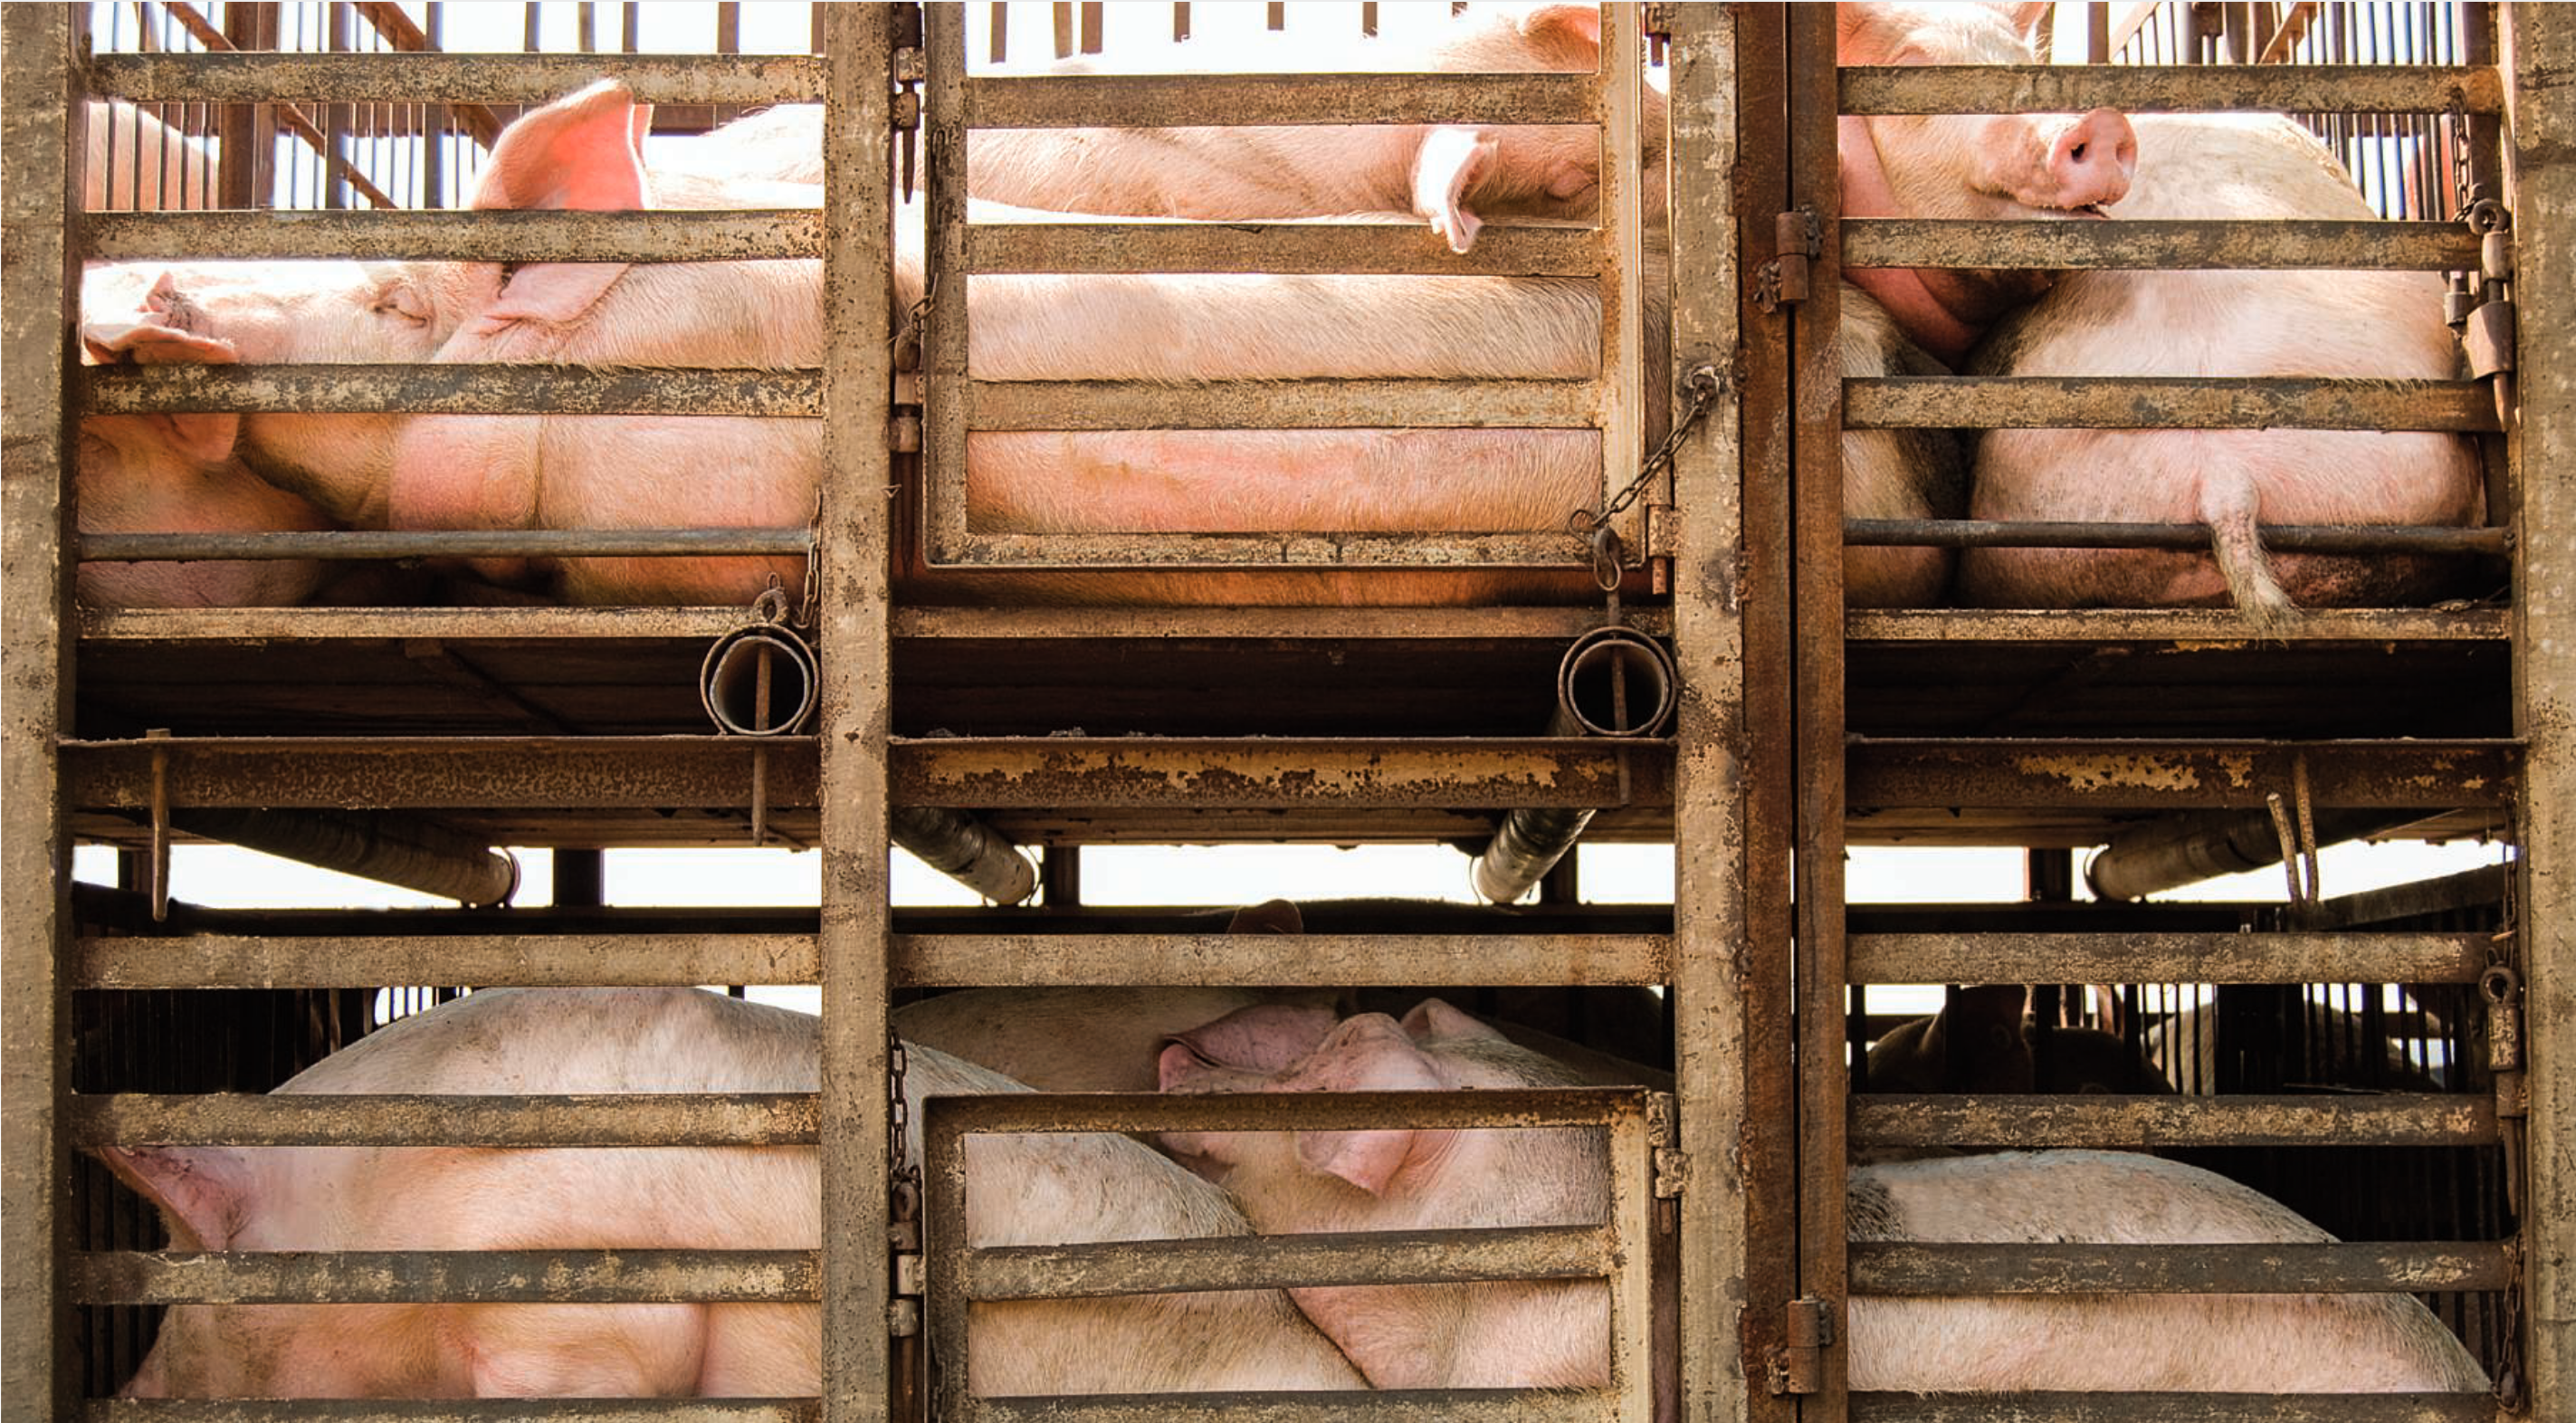
\includegraphics[width=6.25in,height=\textheight]{images/pigs.png}

\textbf{Figure 11. Pigs in cages, Quanzhou, China.} As the largest
consumer of veterinary antimicrobials, China is critical for combating
antimicrobial resistance (AMR). From Van Boekel et
al.\textsuperscript{4}

The reported benefits of using antibiotics for growth promotion is
controversial and supportive data in terms of weight gain is
questionable (1-10\%). Concerns have been expressed that antimicrobial
growth promoters are often used to compensate for poor hygiene/housing
conditions and appropriate healthy veterinary care.\textsuperscript{14}

Unfortunately, use of antibiotic for growth promotion has increased
dramatically with increasing meat-based diets. Since 2000, meat
production has plateaued in high-income countries but has grown by 68\%,
64\%, and 40\% in Africa, Asia, and South America,
respectively.\textsuperscript{4} The transition to high-protein diets in
low- and middle-income countries (LMICs) has been facilitated by the
global expansion of intensive animal production systems, in which
antimicrobials are used routinely to maintain health and productivity.

There are 4 factors that typically determine the health of animals,
(e.g., chickens):

\begin{enumerate}
\def\labelenumi{\arabic{enumi}.}
\tightlist
\item
  The genetic stock of the animals
\item
  Adequate nutrition
\item
  Hygiene of living conditions
\item
  Adequate veterinary care
\end{enumerate}

While antibiotics may be able to improve deficiencies in one area, if
multiple aspects of animal care are missing then antimicrobial
resistance is unlikely to improve animal health or growth. \textbf{Thus,
antimicrobials are often poor surrogates for good hygiene on farms.}
Ideally, a key goal to reduce antibiotic use in animals is to further
strengthen the 4 non-antibiotic aspects that are important to animal
health so antibiotic use can be avoided.

Historically, governmental regulations have focused on toxicological
dose-response data and the presence of antimicrobial residues in animal
tissue, milk or other edible products (i.e.~eggs) from treated animals -
\emph{so called minimum residue levels (MRLs) compatible with acceptable
risk in humans.} While MRLs are well-understood and enforced with
testing programs and penalties, these programs do not take into account
selection of antimicrobial-resistant pathogens.

The WHO has advocated for the termination of using antimicrobials for
growth promotion. A recent
\href{https://www.ecdc.europa.eu/sites/default/files/documents/JIACRA-III-Antimicrobial-Consumption-and-Resistance-in-Bacteria-from-Humans-and-Animals.pdf}{report
from the ECDC} has suggested some progress in addressing this problem.
Using surveillance data from 2017, the EU/EEA population mean antibiotic
consumption in the 29 countries was 130 mg per kg of estimated biomass
in humans and 108.3 mg per kg in food-producing animals. \emph{This
first time since the agencies began publishing the joint reports in 2011
that antibiotic use in humans has exceeded use in livestock.}
Consumption of third- and fourth-generation cephalosporins,
fluoroquinolones, and aminopenicillins was considerably higher in human
medicine, while consumption of macrolides was similar, and consumption
of tetracyclines and polymyxins was significantly higher in
food-producing animals.

In 2022, new
\href{https://eur-lex.europa.eu/legal-content/EN/TXT/PDF/?uri=CELEX:32019R0006\&from=EN}{EU
legislation} will prohibit all forms of routine antibiotic use in
farming, including preventative group treatments and medicated feeding
except in extraordinary circumstances.

\includegraphics[width=6.25in,height=\textheight]{images/livestockabx.png}

\textbf{Figure 12. Antibiotic use in livestock reported in 2010.}
Source: Our World in Data.

\hypertarget{the-impact-of-animal-antibiotic-use-on-human-amr}{%
\subsubsection*{The impact of animal antibiotic use on human
AMR}\label{the-impact-of-animal-antibiotic-use-on-human-amr}}
\addcontentsline{toc}{subsubsection}{The impact of animal antibiotic use
on human AMR}

\hypertarget{case-study-cephalosporins}{%
\paragraph{Case study-cephalosporins:}\label{case-study-cephalosporins}}

Third generation cephalosporins (ceftotaxime, ceftriaxone) are widely
used for serious infections in humans, including the treatment of
urinary tract, abdominal, lung and bloodstream infections. These
antibiotics are classified as ``critically-important'' for human health
(\href{http://www.agisar.org/}{WHO AGISAR}). Ceftiofur, cefpodoxime, and
cefoperazone are similar cephalosporins approved for treating bacterial
infections in food-producing animals including chickens and cattle.

Resistance to 3rd generation cephalosporins is mediated by
extended-spectrum beta-lactamases (ESBLs) and AmpC enzymes. ESBL genes
are transmitted on plasmids, transposons and other mobile genetic
elements that can spread horizontally (surrounding bacteria and
different bacterial species) and vertically (to daughter cells through
replication). In recent years, growing resistance to 3rd generation
cephalosporins in clinical medicine has become so common among
\emph{Escherichia coli} and \emph{Klebsiella pneumonia} that many common
infections are now routinely treated first-line with previously
``last-line'' antibiotics as carbapenems.

A number of studies comparing isolates from animals, food samples, and
human infections have found a high genetic similarity or clonal isolates
that carry the same ESBL genes and plasmids colonizing animals used for
food production and isolates causing clinical infections in
patients.\textsuperscript{15}

In some chicken-producing enterprises, ceftiofur is injected in small
quantities to hatching eggs or chicks as metaphylaxis for
\emph{Escherichia coli} infections and/or yolk sac
infections.\textsuperscript{14} This practice has been shown to select
for cephalosporin resistance in \emph{Salmonella enterica} serovar
Heidelberg- an important cause of severe human illness (salmonella
infection) linked to consumption of contaminated poultry
products.\textsuperscript{16}

\includegraphics[width=6.25in,height=\textheight]{images/chicken_farm.png}

\textbf{Figure 13. Chicken farm in the United States of America.} Image
source: The Guardian

An example of the link between ceftiofur metaphylaxis and infections in
humans is illustrated by experience from Canada. Studies conducted by
the Canadian Integrated Program for Antimicrobial Resistance
Surveillance detected a high degree of temporal correlation in trends of
resistance to ceftiofur and ceftriaxone (a drug of choice for the
treatment of severe cases of salmonelloses in children and pregnant
women) from \emph{Salmonella} Heidelberg strains isolated from patients
with clinical infections and poultry samples collected at retail
stores.\textsuperscript{17} Voluntary termination of ceftiofur
metaphylaxis in hatcheries in the province of Quebec was followed by a
precipitous drop in the prevalence of resistance to ceftiofur;
subsequent reintroduction of ceftiofur in a more limited way was
followed by a return to higher levels of resistance in \emph{Salmonella}
strains.

\includegraphics[width=6.25in,height=\textheight]{images/Canada_ecoli.png}

\textbf{Figure 14. Ceftiofur resistance in chicken and human
\emph{Salmonella} Heidelberg and chicken \emph{E.
coli}.}\textsuperscript{17}

In Japan, voluntary withdrawal of the off-label use of ceftiofur in
hatcheries in 2012 was also associated with significant decrease in
broad-spectrum cephalosporin resistance in \emph{E. coli} from chickens
prepared for cooking. Some other countries (e.g., Denmark) have placed
voluntary restrictions on ceftiofur use. The label claim for day-old
injection of poultry flocks was withdrawn in Europe, while some
countries have banned off-label use of third-generation cephalosporins,
and in other countries there is a requirement that use be restricted to
situations where no other effective approved drugs are available for
treatment.

\textbf{These examples illustrate the danger of using antibiotics for
metaphylaxis in animals from the same class as antibiotics used to treat
infections in humans.} Similar links between antibiotic metaphylaxis and
resistance in human infections have been reported for fluoroquinolones
antibiotics with \emph{Campylobacter jejuni.}\textsuperscript{18}

\hypertarget{case-study--colistin}{%
\paragraph*{Case study- colistin:}\label{case-study--colistin}}
\addcontentsline{toc}{paragraph}{Case study- colistin:}

Colistin is a member of the polymixin class of antibiotics, which have
been used in both human and veterinary medicine for over 50 years. Until
relatively recently, polymyxin antibiotics were rarely prescribed beyond
topical or inhalational therapy in rare cases because of dose-limiting
neurotoxicity and nephrotoxicity of the drugs.

\textbf{The use of intravenous colistin has surged in the last decade as
a last-line antibiotic for carbapenem-resistant \emph{Pseudomonas
aeruginosa}, \emph{Acinetobacter baumannii} and \emph{Klebsiella
pneumoniae.}} Even as human use has increased, colistin continues to be
used in Brazil, Europe and China as a growth promoting and antibiotic
treatment for pigs, poultry and calves.

\begin{itemize}
\item
  In 2014, colistin use in EU member states in animals was higher than
  humans with a reported 485 tonnes- 99.7\% in oral form or oral
  medicated feed. In China, with the world's largest production of pigs
  and poultry, an estimated 12,000 tonnes of colistin was used in the
  food production industry.\textsuperscript{19}
\item
  In 2015, Lui and colleagues reported plasmid-mediated
  colistin-resistance gene, \emph{mcr-1}, in \emph{Escherichia coli}
  isolates obtained from animals, food and human bloodstream infections
  in China.\textsuperscript{19} Alarmingly, the resistance gene has also
  been detected in 5\% of healthy travellers from China in other parts
  of the world.\textsuperscript{20}
\item
  The \emph{mcr-1} gene has also been detected in isolates obtained from
  wildlife and surface water samples, demonstrating environmental
  contamination.\textsuperscript{21}
\item
  Additional plasmid-mediated colistin-resistance genes have been
  reported in many other bacterial species and countries, including
  \emph{mcr-2} from pigs in Belgium, and \emph{mcr-3,4,5} in other
  countries.\textsuperscript{22}
\item
  Colistin illustrates important \emph{One-Health Dimensions} \emph{of
  AMR} that differ from third generation
  cephalosporins.\textsuperscript{23} Use of large quantities of
  colistin for group treatment or growth promotion in animals has
  probably lead to antimicrobial resistance problems in human health,
  even through colistin was considered in the past to be less important
  because other less toxic treatments were still available.
\item
  In 2017, China banned the use of colistin as a food additive for
  animals. Colistin is currently not approved as a food additive in
  Europe or the United States, but is still be used in LMICs as a growth
  promoting agent because of its low cost.
\end{itemize}

\hypertarget{antimicrobial-resistance-in-animals-in-lmics}{%
\subsubsection*{Antimicrobial resistance in animals in
LMICs}\label{antimicrobial-resistance-in-animals-in-lmics}}
\addcontentsline{toc}{subsubsection}{Antimicrobial resistance in animals
in LMICs}

Many farmers in LMICs are sustenance farmers, and their livelihood is at
stake if an animal becomes ill.~Therefore, they may not have the
resources for optimally nutritious feed and housing space/conditions.
These challenges, combined with looser regulations on veterinary drugs,
lead to often liberal use of antibiotic in animal feed to ensure animal
health.\textsuperscript{4}

\includegraphics[width=6.25in,height=\textheight]{images/livestock_LMIC.png}

\textbf{Figure 15. Global hotspots of antimicrobial resistance in
animals.} Data source
\href{https://resistancebank.org/}{resistancebank.org}

The largest hotspots of AMR in animals were in Asia and India. Asia is
home to 56\% of the world's pigs and 54\% of the chickens. Other growing
hotspots of AMR are found in central India and Kenya, where resistance
to multiple drugs has appeared but not yet reached 50\%.

These data suggest that in areas such as Asia, targeted interventions
such as legislative action and subsidies to improve farm hygiene could
reduce the need for antimicrobials in animal production, thereby
preserving important drugs for human medicine and the treatment of sick
animals. In these regions, meat consumption is still low, but animal
production is gradually increasing. Here, there may be a window of
opportunity to contain AMR by imposing strict hygiene standards in newly
built farms. This approach could reduce the risk of the spread of
resistant pathogens such as \emph{mcr} 1--carrying \emph{E. coli} that
have emerged in regions where intensive meat production has been
facilitated by enormous quantities of veterinary antimicrobials.

In Africa, resistance maps reveal the absence of major AMR hotspots,
except for the Johannesburg metropolitan area. This suggests, on the
basis of the regions surveyed, that Africa probably bears
proportionately less of the current global burden of AMR than high- and
upper- to middle income countries. Policy-makers coordinating an
international response to AMR might therefore spare Africa from the most
aggressive measures, which may undermine livestock-based economic
development and rightfully be perceived as unfair.

Clearly the the transition to sustainable animal production in both HIC
and LMICs with improvements in farm-level biosafety and biosecurity are
essential to reduce the future risk of AMR.

\begin{longtable}[]{@{}
  >{\raggedright\arraybackslash}p{(\columnwidth - 0\tabcolsep) * \real{1.0000}}@{}}
\toprule
\endhead
\textbf{For further study:} In the 1990s avoparcin, a glycopeptide
antimicrobial, was widely used in growth promotion in pigs and poultry
production that was not initially thought to be of public health
importance. Surveillance and research were eventually able to show that
avoparcin use in animals contributed to the selection and wide
dissemination of what type of resistance? \\
\bottomrule
\end{longtable}

\hypertarget{environmental-concerns}{%
\subsubsection*{Environmental concerns}\label{environmental-concerns}}
\addcontentsline{toc}{subsubsection}{Environmental concerns}

One Health considers possible environmental drivers of AMR in additional
to human and animal health.\textsuperscript{14} Many resistance
mechanisms such as beta-lactamases are millions of years old and
pre-date antibiotics. Soil and other environmental sources are rich
sources of highly-diverse populations of bacteria and genes.

Antimicrobial resistance to a wide variety of drugs has been
demonstrated in environmental bacteria isolated from the pre-antibiotic
era, as well as from various sites on every continent free of other
sources of exposure to modern antimicrobials. \textbf{Yet there is
abundant evidence that human antibiotic use is having an impact on the
\emph{resistome}- the totality of or resistance genes in the total
environment}.\textsuperscript{24}

\textbf{Hundreds of thousands of tonnes of antimicrobials are produced
annually and find their way into the environment. Waste from treatment
plants and the pharmaceutical industry, if inadequately treated, can
release high concentrations of antimicrobials into surface water.}
Residues and metabolites of antimicrobials are constituents of human
sewage, livestock manure, and aquaculture, along with fecal bacteria and
resistance genes. Sewage treatment and composting of manure reduce
concentrations of some, but not all antimicrobials and micro-organisms,
which are introduced to soil upon land application of human and animal
bio-solids.\textsuperscript{25}

\begin{itemize}
\tightlist
\item
  In developed countries with good-quality sewage and drinking water
  treatment, and where most people have little to no direct contact with
  food-producing animals, transmission of bacteria and resistance genes
  from agricultural sources is largely foodborne, either from direct
  contamination of meat and poultry during slaughter and processing, or
  indirectly from fruit and vegetables contaminated by manure or
  irrigation water.
\item
  In countries with poor sewage and water treatment, drinking water is
  likely to be very important in the transmission of resistant bacteria
  and/or genes from animals. Poor sanitation also facilitates indirect
  person-person water-borne transmission of enteric bacteria among
  residents as well as international travellers who return home
  colonized with resistant bacteria acquired locally.
\item
  Through these and other means, including globalized trade in animals
  and food and long-distance migratory patterns of wildlife can spread
  AMR worldwide rapidly.
\end{itemize}

General measures to address antimicrobial resistance in the wider
environment include improved controls on pollution from industrial,
residential, and agricultural sources. Improved research as well as
environmental monitoring and risk assessment are also required to better
understand the role of the environment in the selection and spread of
antimicrobial resistance, and to identify more effective strategies to
address resistance in this sector.

\includegraphics[width=6.25in,height=\textheight]{images/hotspots.png}

\textbf{Figure 16. Hotspots of antimicrobial resistance.} Figure is from
Singer et al.\textsuperscript{26}

\newpage

\hypertarget{cross-border-spread-of-amr}{%
\subsection*{Cross-border spread of
AMR}\label{cross-border-spread-of-amr}}
\addcontentsline{toc}{subsection}{Cross-border spread of AMR}

\includegraphics[width=6.25in,height=\textheight]{images/worldairlineroute2014.png}

\textbf{Figure 17. World airline travel routes in 2014.} Photo credit
Jpatokal/Wikimedia (CC BY-SA 2.5)

The COVID-19 pandemic has exposed the limitations of global
collaboration and response within existing global health frameworks,
pointing to a clear need for more rules-based global governance to be
able to effectively prevent, prepare and respond to health emergencies
in a more just equitable way. However, valuable lessons from COVID-19
pandemic could enhance actions against AMR. Clearly, actions taken by
one country have had substantial consequences for others. Governments
should significantly bolster global and national capacity to prevent and
respond to global cross-border health threats more broadly.

\textbf{Table 3. Global successes and shortcomings in the multilateral
response to the COVID-19 pandemic.} Table is from Jit et al
2021.\textsuperscript{11}

\begin{longtable}[]{@{}
  >{\raggedright\arraybackslash}p{(\columnwidth - 4\tabcolsep) * \real{0.1688}}
  >{\raggedright\arraybackslash}p{(\columnwidth - 4\tabcolsep) * \real{0.4586}}
  >{\raggedright\arraybackslash}p{(\columnwidth - 4\tabcolsep) * \real{0.3726}}@{}}
\toprule
\begin{minipage}[b]{\linewidth}\raggedright
Domain
\end{minipage} & \begin{minipage}[b]{\linewidth}\raggedright
Successes
\end{minipage} & \begin{minipage}[b]{\linewidth}\raggedright
Shortcomings illustrated by COVID-19 pandemic
\end{minipage} \\
\midrule
\endhead
\textbf{Research collaboration and information sharing} &
\begin{minipage}[t]{\linewidth}\raggedright
\begin{itemize}
\item
  Sharing of information by researchers
\item
  International research collaborations
\item
  Public data repositories
\end{itemize}
\end{minipage} & \begin{minipage}[t]{\linewidth}\raggedright
\begin{itemize}
\item
  Many regions and countries slow to learn policy lessons from elsewhere
\item
  Lack of systemic global research governance
\item
  Duplication of research studies
\end{itemize}
\end{minipage} \\
\textbf{Vaccine discovery and development} &
\begin{minipage}[t]{\linewidth}\raggedright
\begin{itemize}
\item
  Multinational initiatives to fund efforts such as the Coronavirus
  Global Response and the Coalition for Epidemic Preparedness
  Innovations
\item
  Approval of vaccines and adjuvants
\item
  Establishing the principle of equitable vaccine distribution through
  the COVAX Facility (despite failures in implementation)
\end{itemize}
\end{minipage} & \begin{minipage}[t]{\linewidth}\raggedright
\begin{itemize}
\item
  Most funding from national efforts
\item
  Most vaccine doses secured by rich countries through bilateral deals
\item
  Trade barriers around vaccines and raw materials
\end{itemize}
\end{minipage} \\
\textbf{Travel policies} & \begin{minipage}[t]{\linewidth}\raggedright
\begin{itemize}
\tightlist
\item
  Travel restrictions delayed spread from China in early 2020
\end{itemize}
\end{minipage} & \begin{minipage}[t]{\linewidth}\raggedright
\begin{itemize}
\item
  Dissonant COVID-19 response policies between highly connected nations
  (e.g., Scandinavia)
\item
  Restrictions on travel to countries of high COVID-19 incidence
  contribute little to control in these countries
\end{itemize}
\end{minipage} \\
\bottomrule
\end{longtable}

\textbf{The actions of the EU during the pandemic illustrate the tension
between short-term nationalistic incentives and long-term imperatives
for cooperation towards achieving global public goods such as equitable
distribution of vaccines or reducing antimicrobial resistance.} The EU
has struggled to balance preferences of individual member-states (and
those of their political leaderships) with the collective interests of
all member-states. Such tensions are especially challenging when health
care and health policy issues are involved, given how these have
decisions in the past have largely remained the responsibility of the
member-states. In a pandemic, this can lead to inertia and political
indecisiveness at the EU level, with member-states filling the gap with
potentially contradictory or competing decisions.

Looking ahead, it is likely that there will be several changes to the
global health architecture, possibly including a new WHO pandemic treaty
in 2022 and additional international collaborative mechanisms to promote
preparedness and coordinate responses to future pandemics. In the
subsequent modules, we explore what those developments might look like
in three key areas.

\hypertarget{summary}{%
\subsection*{Summary}\label{summary}}
\addcontentsline{toc}{subsection}{Summary}

The post-COVID-19 world must overcome the serious setbacks from the
pandemic to hard-fought progress in reducing poverty and inequality.
Health infrastructure and human resources vital for fighting AMR have
been overburdened and will take many years to recover, particularly if
governments impose austerity measures as they seek to recover from
fiscal expansion during the pandemic.

Decades of funding neglect, combined with continuously increasing global
antibiotic consumption, poor surveillance data, and weak pipelines for
new drugs, vaccines and diagnostics, has left the world dangerously
vulnerable to a pandemic of antibiotic-resistant and untreatable
infections.

\textbf{Therefore, strong multilateral collaboration is essential for
the world to absorb these shocks and refocus on the silent but growing
pandemic of AMR.} Pandemics are opportunities to re-imagine governance
structures and learn from previous experiences. COVID-19 has shown the
importance of multilateral collaboration in diverse areas, including
research and knowledge sharing, discovery, development and distribution
of vaccines and medicines and access to diagnostics and medicines.
Action is needed now to reverse the unthinkable future of untreatable
infections.

\hypertarget{module-2-the-public-health-crisis-of-new-antibiotic-development}{%
\section*{Module 2: The Public Health Crisis of New Antibiotic
Development}\label{module-2-the-public-health-crisis-of-new-antibiotic-development}}
\addcontentsline{toc}{section}{Module 2: The Public Health Crisis of New
Antibiotic Development}

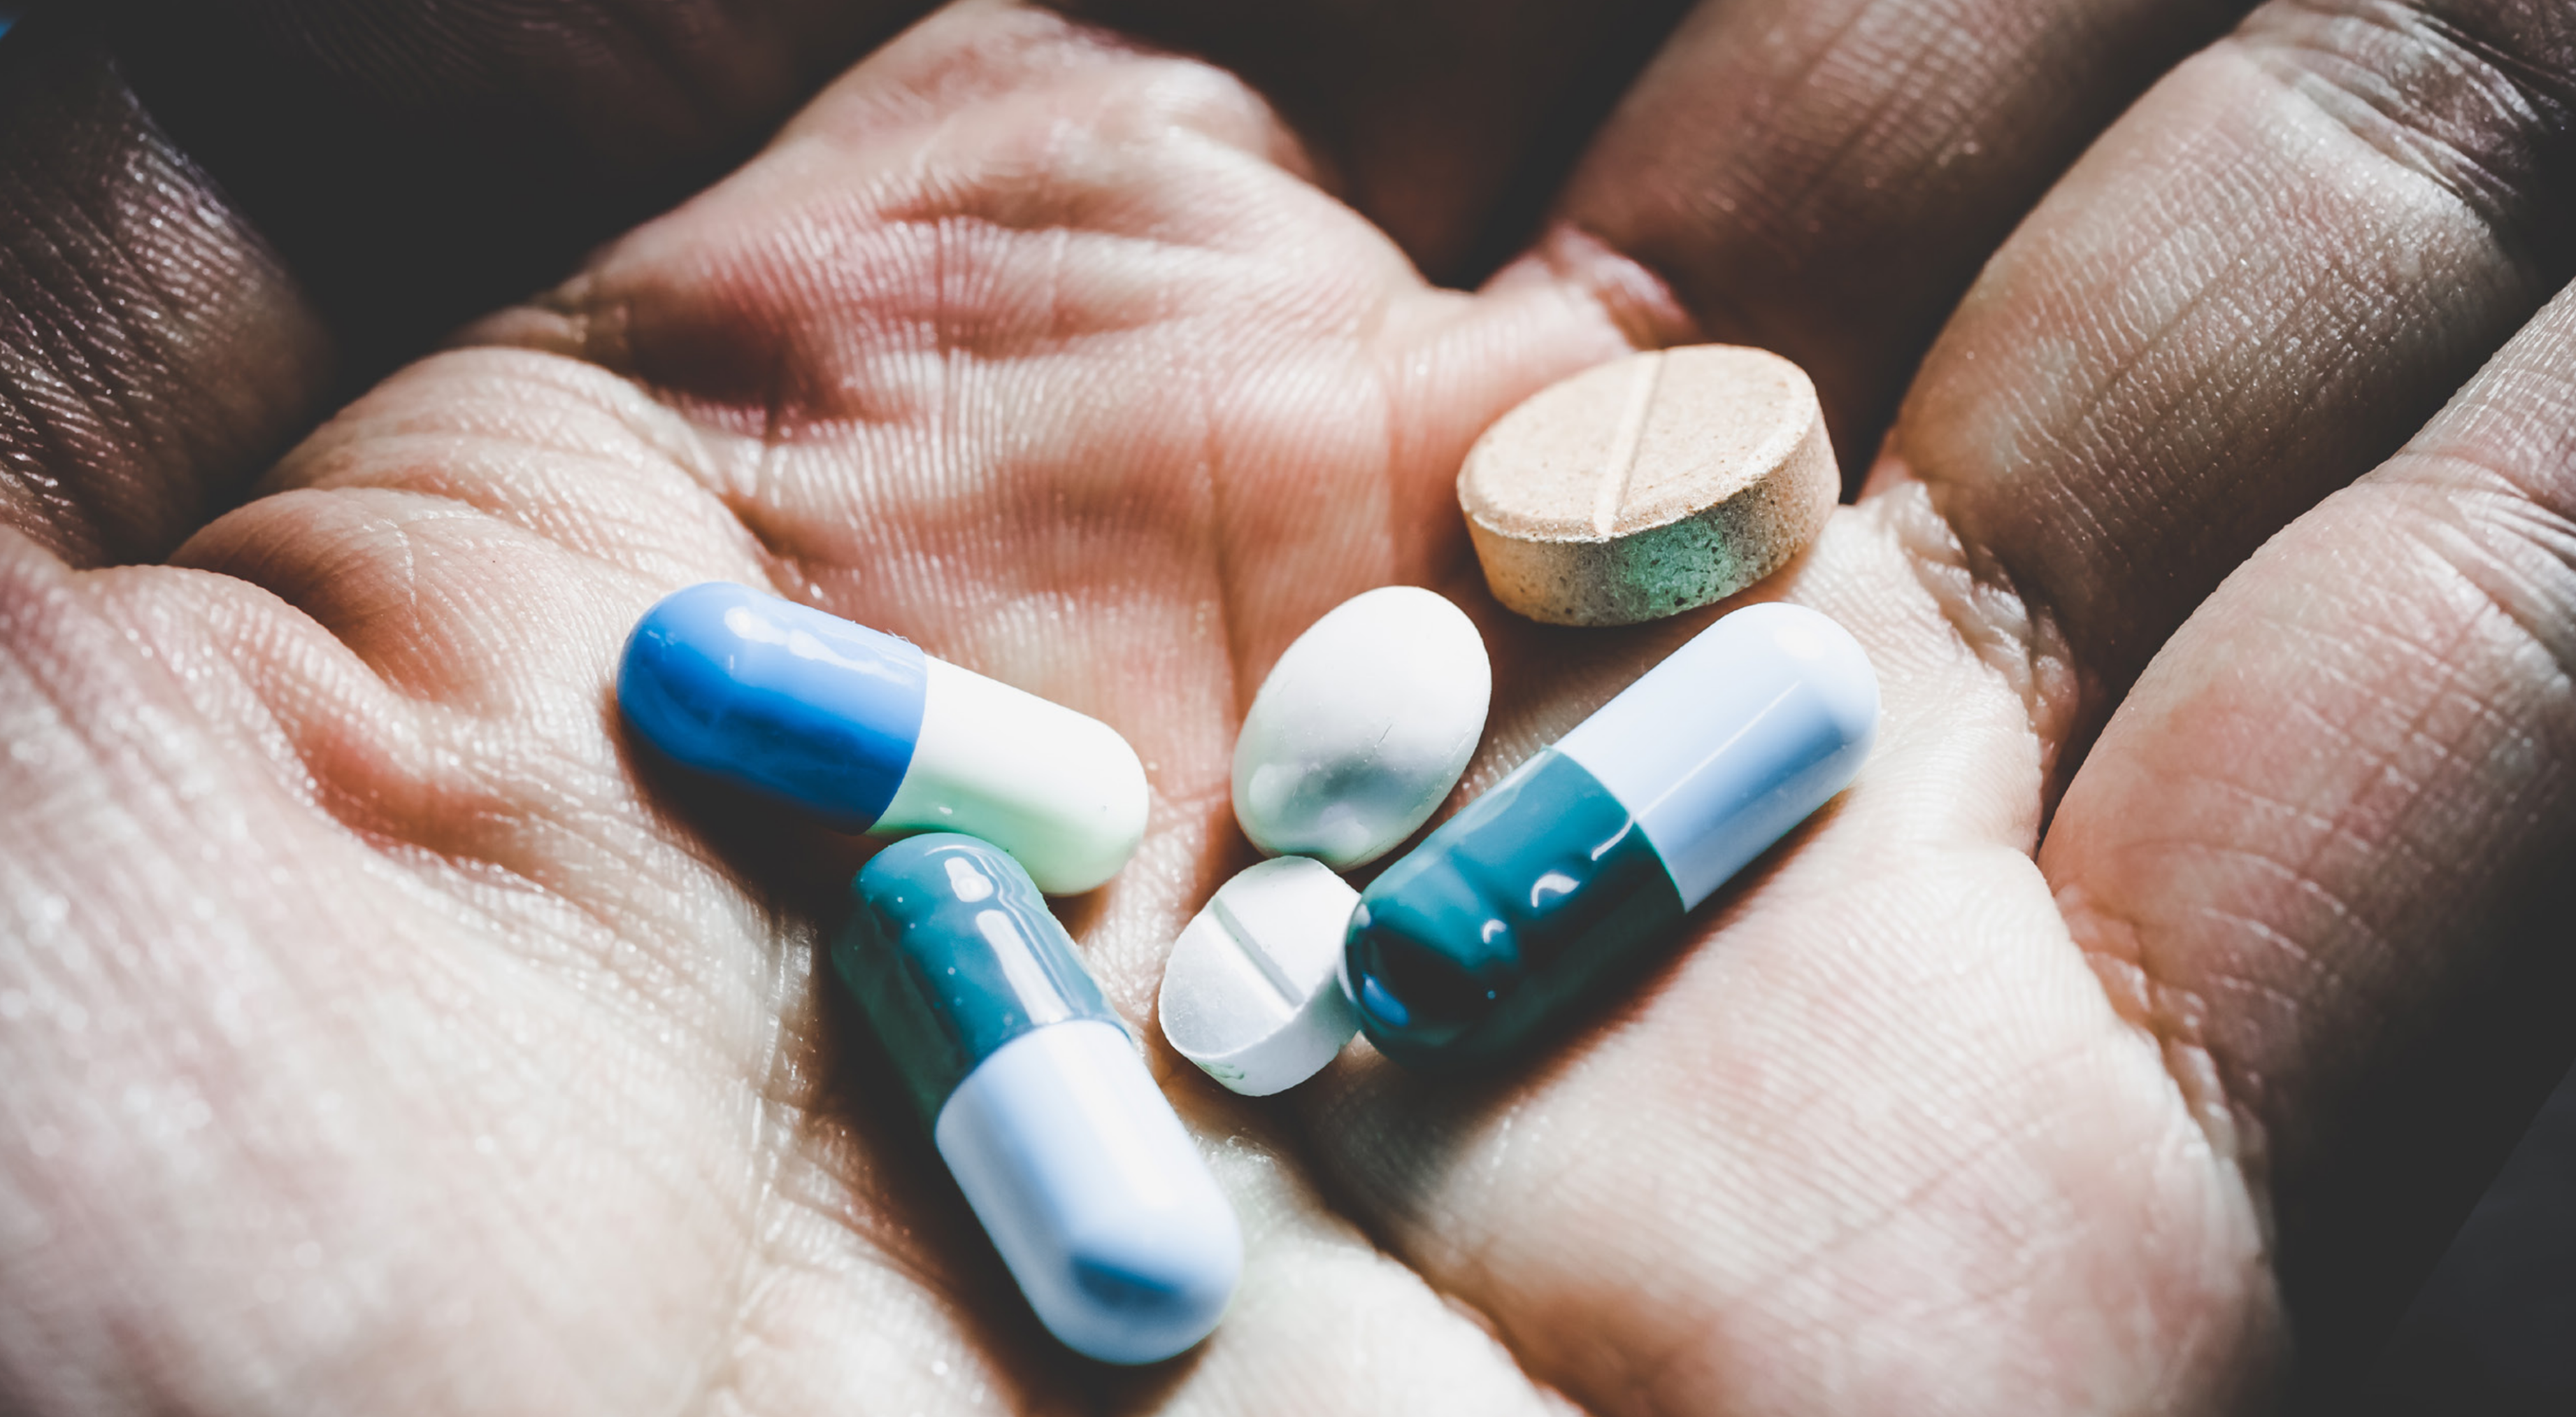
\includegraphics[width=6.25in,height=\textheight]{images/antibiotics.png}

\hypertarget{background}{%
\subsection*{Background}\label{background}}
\addcontentsline{toc}{subsection}{Background}

In module 1, we discussed the history of antibiotic discovery and the
current challenges with antimicrobial resistance that has been worsened
by the lack of new antibiotic development. In this module, we will
examine the scientific and economic challenges associated with
antibiotic discovery and regulatory approval, and compare and contrast
strategies that have been proposed to stimulate the antibiotic pipeline.

As discussed in Module 1, antibiotic discovery began to slow in the
1980's leading to a discovery void in new molecular entities (NMEs)
since the 1990s. This lack of antibiotic innovation occurred at a
critical period when antibiotic resistance, particularly to many
front-line beta-lactam antibiotics, began to increase rapidly due to the
emergence and worldwide diffusion of new forms of enzymatic
(beta-lactamase) resistance to antibiotics. These bacterial enzymes can
be broadly classified as:

\begin{itemize}
\tightlist
\item
  Narrow-spectrum beta-lactamases, which act on penicillins and
  first-generation cephalosporins (e.g., TEM-1 and 2, SHV-1,
  cephalosporinases, OXA-type enzymes
\item
  Extended-spectrum beta-lactamases (ESBLs), which act on penicillins
  and all four generations of cephalosporins (e.g., SHV-2, SHV-5, SHV-7,
  SHV-12, TEM-10, TEM-12, TEM-26, CTX-M, OXA-type ESBLs)
\item
  Carbapenemases, which act on penicillins, all four generations of
  cephalosporins, and carbapenems (e.g., KPC, NDM-1, VIM and IMP
  carbapenemases, OXA-type carbapenemases).
\end{itemize}

The emergence and rapid spread of these beta-lactamases was problematic
because they have a low barrier for further mutation and creating
resistance to new beta-lactams that are used as first and second line
therapies for common respiratory, abdominal, and genital-urinary tract
infect infections. Additionally, many of these enzymes are encoded on
spread on plasmids (mobile genetic elements that can be passed from one
bacterial species to another) that harbour additional resistance
mechanisms to other antibiotic classes leading to the emergence and
rapid dissemination of multidrug resistance.

\includegraphics[width=4.16667in,height=\textheight]{images/betalactamases.png}

\textbf{Figure 1. Increase in numbers of group 1, 2, and 3
beta-lactamases from 1970 to 2009}.\textsuperscript{27}

In 2017 the WHO convened a group of experts to prioritize the need for
new drugs to treat antibiotic- resistant bacteria. The WHO assigned the
highest priority to antibacterial drug research and development for the
Gram- negative bacteria \emph{Acinetobacter}, \emph{Pseudomonas} and
species of \emph{Enterobacterales} that are resistant to carbapenems and
are usually extensively drug resistant (XDR).

\textbf{Table 1. WHO priority pathogens}

\begin{longtable}[]{@{}
  >{\raggedright\arraybackslash}p{(\columnwidth - 2\tabcolsep) * \real{0.1389}}
  >{\raggedright\arraybackslash}p{(\columnwidth - 2\tabcolsep) * \real{0.8611}}@{}}
\toprule
\begin{minipage}[b]{\linewidth}\raggedright
Priority
\end{minipage} & \begin{minipage}[b]{\linewidth}\raggedright
Pathogens included
\end{minipage} \\
\midrule
\endhead
\textbf{Critical} & \emph{Acinetobacter baumannii}
(Carbapenem-resistant)

\emph{Pseudomonas aeruginosa} (Carbapenem-resistant)

Enterbacterales (3rd generation cephalosporin, carbapenem-resistant) \\
\textbf{High} & \emph{Enterococcus faecium}, vancomycin-resistant

\emph{Staphylococcus aureus}, methicillin-resistant, vancomycin
intermediate and resistant

\emph{Helicobacter pylori}, clarithromycin-resistant

\emph{Campylobacter}, fluoroquinolone-resistant

\emph{Salmonella} spp., fluoroquinolone-resistant

\emph{Neisseria gonorrhoeae}, 3rd generation cephalosporin-resistant,
fluoroquinolone-resistant \\
\textbf{Medium} & \emph{Streptococcus pneumoniae},
penicillin-non-susceptible

\emph{Haemophilus influenzae}, ampicillin-resistant

\emph{Shigella} spp., fluoroquinolone-resistant \\
\bottomrule
\end{longtable}

The same year, the WHO released a
\href{https://apps.who.int/iris/bitstream/handle/10665/330420/9789240000193-eng.pdf}{clinical
pipeline report}, which was updated in 2018 and 2019. The report
analysed antibiotics and biologics in development according to their
activity against the critical priority pathogens carbapenem resistant
\emph{Acinetobacter baumannii} (CRAB), carbapenem-resistant
\emph{Pseudomonas aeruginosa} (CRPA), extended spectrum beta-lactamase
(ESBL) producing Enterobacterales and carbapenem resistant
Enterobacterales (CRE). The level of innovation in the global clinical
pipeline was assessed on the basis or the absence of pre-existing
cross-resistance to currently used antibacterial drugs. The key findings
from this report were:

\begin{quote}
\begin{itemize}
\item
  The clinical pipeline remains insufficient to tackle the challenge of
  increasing emergence and spread of antimicrobial resistance.
\item
  It is primarily driven by small- or medium-sized enterprises (SMEs),
  with large pharmaceutical companies continuing to exit the field.
\item
  Eight new antibacterial agents have been approved since 1 July 2017,
  but overall, they have limited clinical benefits.
\item
  One new anti-tuberculosis (anti-TB) agent, pretomanid, developed by a
  not-for-profit organization, has been approved for use within a set
  drug-combination treatment for MDR TB.
\item
  The current clinical pipeline contains 50 antibiotics and combinations
  (with a new therapeutic entity) and 10 biologicals, of which 32
  antibiotics are active against the WHO priority pathogens:

  \begin{itemize}
  \item
    Six of these agents fulfil at least one of the innovation criteria;
    only two of these are active against the critical MDR Gram-negative
    bacteria.
  \item
    More than 40\% of the pipeline targeting WHO priority pathogens
    consists of additional beta-lactam and beta-lactamase inhibitor
    (BLI) combinations, with a major gap in activity against
    metallo-beta-lactamase (MBL) producers.
  \item
    The anti-TB and \emph{Clostridium difficile} antibacterial pipeline
    is more innovative than the WHO priority pathogens pipeline, with
    more than half of the antibiotics fulfilling all of the innovation
    criteria.
  \end{itemize}
\end{itemize}
\end{quote}

The report confirms previous reports and highlights the public health
implications of a drying antibiotic pipeline. In the following sections
we will explore the causes and potential solutions to this crises.

\hypertarget{why-has-antibiotic-discovery-faltered-in-recent-years}{%
\subsection*{Why has antibiotic discovery faltered in recent
years?}\label{why-has-antibiotic-discovery-faltered-in-recent-years}}
\addcontentsline{toc}{subsection}{Why has antibiotic discovery faltered
in recent years?}

\hypertarget{scientific-challenges}{%
\subsubsection*{Scientific challenges}\label{scientific-challenges}}
\addcontentsline{toc}{subsubsection}{Scientific challenges}

Discovering new antibiotics is inherently challenging. Antibiotics must
attack multiple target bacterial species that change over time by
developing resistance, and must reach effective concentrations in
multiple body compartments.\textsuperscript{1} The discoverer of a new
antibiotic must guess what resistance mechanisms will be a problem in 10
years, and bring drugs to market to overcome these mechanisms. This
flexibility and risk is not encountered in other therapeutic areas such
as hypertension, diabetes, hyperglycemia, or Alzheimer's disease where
the drugs bind to one specific target. Even for cancer chemotherapy,
which develops resistance to therapy, the mechanisms leading to
resistance are not transmissible to other cancers or patients.
Antibiotics must also be remarkably non-toxic, as their daily dosages
often measured in \emph{grams} not \emph{milligrams} as is the case for
other pharmaceuticals.

Nearly all of the antibiotics used today belong to classes of drugs
discovered before 1970. They are products of a ``golden age'' of
antibiotic discovery from 1945-1965, which screened natural products
from soil streptomyces and fungi. This discovery approach hit the law of
diminishing returns by the 1960's with the same classes of antibiotics
being consistently rediscovered.\textsuperscript{1} Put simply, the
\emph{low-hanging} fruit for discovering new antibiotics has already
been picked. Since 1970, the only new antibiotic classes to reach the
marked are the oxazolidinediones (i.e.~linezolid discovered in 1978
launched in 2000) and lipopeptides (discovered in 1986 launched in
2003).

Most improvements in antibiotics since the 1970s have come through
modification of existing antibiotic classes yielding analogues with
increased potency and greater ability to evade existing resistance
mechanisms. However, over time this approach has become more difficult
with the emergence of more potent resistance mechanisms that affect
multiple antibiotics within the same classe.

Given the the limits of existing strategies of screening soil organisms,
the pharmaceutical industry turned to genomics-based high-throughput
antibiotic discovery strategies with considerable enthusiasm in the
1990s.\textsuperscript{1} This discovery leveraged genomic sequence data
from several target bacterial pathogens to identify conserved genes
encoding ``essential pathways'' in bacteria not found in mammalian
cells, and then used high-throughput inhibition screens of existing
chemical compound libraries to identify ``druggable'' molecules for
these genetic targets/pathways.

\textbf{Despite early enthusiasm and huge financial investments by many
pharmaceutical companies, very few potential new antibiotic targets were
identified and even fewer drugs entered into clinical development.} An
example of the scientific challenge is illustrated by experience of
SmithKline Beecham (later purchased by Glaxo Smith Kline-one of the few
large pharmaceutical companies still involved in antibiotic discovery.
Indeed, only four major pharmaceutical companies still have active
antibiotic research programmes.

\begin{longtable}[]{@{}
  >{\raggedright\arraybackslash}p{(\columnwidth - 0\tabcolsep) * \real{1.0000}}@{}}
\toprule
\endhead
\textbf{The disappointment of genomics:} From 1995 to 2002, SmithKline
Beecham (now part of GlaxoSmithKline (GSK) identified 300 potential
targets and ran 67 high-throughput screens, each of 260,000 --530,000
compounds. Sixteen screens led to `hits'---meaning compounds that bound
selectively to a target giving a reproducible positive signal in the
assays---and five of these translated into `lead' compounds. Of the five
corresponding targets, two (FabI9 and Mrs) were not universally
essential or conserved, meaning that they could not be developed as
broad-spectrum antibiotics, and it proved impossible to incorporate
`drug-like properties' into molecules that bound two others. The final
target identified was peptide deformylase, for which GSK now has a
molecule (GSK 1322322) in Phase II trials, although this did not come
from high-throughput genomic-based screening. This performance appears
typical of other companies that followed the genomics strategy of
antibiotic discovery. Thus, 20 years after its advent, no antibiotic
developed by genomic screening has reached the
market.\textsuperscript{28} \\
\bottomrule
\end{longtable}

\hypertarget{antibiotic-regulatory-hurdles}{%
\subsubsection*{Antibiotic regulatory
hurdles}\label{antibiotic-regulatory-hurdles}}
\addcontentsline{toc}{subsubsection}{Antibiotic regulatory hurdles}

The goal of regulatory bodies such as the U.S. Food and Drug
Administration (FDA), the European Medicines Agency (EMA), and the
African Medicines Agency (AMA) is to review the potential benefits and
risks to ensure that new drugs that make it to market are both safe and
effective for patients in need. Still, a drug that gains FDA approval
may give pause to European reviewers, despite having reviewed the same
evidence as their American counterparts, and vice versa. Both the
\href{https://www.fda.gov/media/82381/download}{FDA} and the
\href{https://www.ema.europa.eu/en/documents/other/laboratory-patient-journey-centrally-authorised-medicine_en.pdf}{EMA}
and
\href{https://www.ifpma.org/subtopics/african-medicines-agency/}{AMA}
have distinct processes with different methods of endpoint evaluation,
and individual comfort levels with risk. Other countries, such as
\href{https://cdsco.gov.in/opencms/opencms/en/Drugs/New-Drugs/}{India}
and
\href{https://www.appliedclinicaltrialsonline.com/view/regulatory-requirements-and-key-points-drug-clinical-trials-registration-china}{China}
and many LMICs have their own processes for drug registration.
\textbf{Therefore, if a new antibiotic that is effective for treating
MDR pathogens is approved in one country, there is no guarantee that the
drug will be favourably reviewed or available in other countries.}

Less than 10\% of LMICs have access to ``newly- approved'' antibiotics
within 10 years of approval in teh U.S. or EU, due to low expectation of
revenues in these smaller markets.\textsuperscript{29} This is despite
the fact that the majority of the world's annual 5.7 million
antibiotic-treatable deaths occur in LMICs.\textsuperscript{30} Even in
HIC, patient access to new antibacterials is limited in countries such
as Canada, Japan, and many European countries.\textsuperscript{31} If
truly innovative antibacterials, like those identified by WHO, cannot
find profitable markets, they will not be developed in the future.

LMICs with limited drug regulatory capacity have poor control of
antibiotic distribution. As a result, some antibiotics that should be
reserved as a last-line treatment option are sold without a
prescription. Limited regulatory capacity may also lead to rampant
availability of sub-standard and falsified (counterfeit) antibiotic
products, which further promote the emergence of antibiotic-resistant
pathogens. \emph{The issue surrounding counterfeit antibiotics will be
discussed in more detail in Module 3.}

\includegraphics[width=6.25in,height=\textheight]{images/clinical trial.png}

\textbf{Figure 2. Pathway from drug discovery to regulatory approval and
estimated costs.} ADMET- studies to document drug absorption,
distribution, metabolism and elimination, and toxicity in animals. PK/PD
pharmacokinetic/pharmacodynamic relationships- i.e.~dose response and
toxicity relationships from animals.

A company seeking regulatory approval to sell a new prescription
antibiotic must complete a five-step process: discovery/concept,
preclinical research (animal testing), clinical research, regulatory
review, and post-market safety monitoring. \textbf{The cost to achieve
this regulatory approval for antibiotics has been estimated between 1 to
1.5 billion dollars}.\textsuperscript{32} The two most expensive phases
in antibiotic development are drug discovery (due to the high failure
rate) and clinical trials. Current guidance published by the US Food and
Drug Administration (FDA) and the European Medicines Agency (EMA)
requires randomized controlled clinical trials to demonstrate the
non-inferiority of the new antibiotic to established therapies. This has
to be complemented by the enrolment of a large number of patients to
support the marketing application (New Drug Application NDA or Marketing
Authorization Application MAA, respectively) for 1 or more infection
site--specific indication (e.g., complicated urinary tract infection or
complicated intra-abdominal infection), based on the drug's clinical
efficacy and safety. The bacterial pathogens relevant to the indication
listed in the prescribing information are a \emph{secondary
consideration} based on the spectrum of activity of the investigational
antibiotic and the microbiological data from patients collected during
clinical trials.\textsuperscript{33} \textbf{As a result, even if a new
antibiotic is developed for a MDR pathogen, it is not possible to
perform clinical studies and receive approval from the FDA or EMA for an
indication of treating MDR pathogens.}

Despite these high risks and costs, the returns to the innovator and
investor for approved antibiotics are relatively poor. Profitability is
often not realized before the 20-year exclusive patent
expires.\textsuperscript{34} Industry analysts estimate that the average
revenue generated from an antibiotic's sale is roughly \$46 million per
year.\textsuperscript{32} \textbf{The fundamental problem for
antibiotics is that their development is not profitable} compared to
other therapeutic areas.

\includegraphics[width=6.25in,height=\textheight]{images/antibioticprofit.png}

\textbf{Figure 3. Profitability of the antibiotic sector vs.~other drug
types.} Source: Financial Times

Moreover, it is difficult for an antibiotic manufacturer to be able to
precisely identify the small proportion of patients who both really need
the antibiotic for a MDR pathogen and are willing to pay a high price
for the drug. As noted by Ardal and colleagues:\textsuperscript{35}

\begin{quote}
The major challenge with antibiotics is profitability. As older
antibiotics are still effective for treating most infections, the
primary value of new antibiotics is to treat multidrug-resistant (MDR)
infections and provide a protective benefit against emerging pathogens.
The duration of antibiotic treatment for individual patients is
relatively short (for example, 1--2 weeks or up to 1 month), whereas the
treatment for chronic conditions such as hypertension or hyperlipidemia
can be continuous over many years. Resistance is hastened by use, new
antibiotics are stewarded as a last resort, which results in low unit
sales. Whereas medicines for rare diseases have used high unit-pricing
strategies to achieve profitability, these are often unavailable to
antibiotic developers due to clinical trial design (it is difficult to
demonstrate the superiority of new antibiotics as resistance is still
relatively uncommon) and bundled hospital reimbursement structures
(whereby hospitals are incentivized to prescribe lower-cost
antibiotics). Large pharmaceutical companies have largely abandoned the
market, accounting for only 4 of the 42 antibiotics currently under
development.\textsuperscript{36} Any investment in a new antibiotic is
seen as a high-risk proposition, and consequently the returns expected
by prospective investors are high to account for this risk premium. This
in turn puts pressure on small and medium-sized enterprises (SMEs), as
there is little chance that their candidate -antibiotics will be
purchased by larger companies.
\end{quote}

Enormous costs are also incurred once an antibiotic is approved as
regulatory agencies make registration and marketing contingent on
post-approval obligatory (phase IV) studies: pediatric dosing and safety
studies, pharmacokinetic studies in special populations (i.e.~elderly,
obese, dialysis), pharmacovigalence (safety), development and validation
of susceptibility testing technology, manufacturing and supply chain
investments, and a 5-10 years commitment to monitor resistance through
antimicrobial surveillance studies. Recouping these costs may be
impossible for drugs with activity against MDR pathogens as many many
countries and health systems will negotiate the lowest possible price
for purchase and then (appropriately) restrict the use of the antibiotic
to preserve its effectiveness- resulting in low sales. This is
completely different from a scenario of a new ``breakthrough'' cancer
therapy, where the drug will be immediately incorporated in treatment
algorithms for eligible patients.

Fundamentally, the math problem of antibiotic profitability can be
summarized as:

\(Costs= Antibiotic \ Price * Units\ Sold\)

The only way to recover the investment in antibiotics is to either
charge very high prices for the antibiotic or to sell/use lots of
antibiotic, thus driving resistance. Both options are difficult to
justify to patients.

\includegraphics[width=6.25in,height=\textheight]{images/profitability.png}

\textbf{Figure 4. Delayed profitability post antibiotic approval.}
Source McKenna et al.\textsuperscript{34}

While the high post-approval costs may be absorbable by large
pharmaceutical companies with other profitable drug products in other
therapeutic areas, they can put smaller companies out of business. The
company must pay for the high post-approval costs described above that
for antibiotics cannot be covered through aggressive sales. For
antibiotics, companies have no way to pay for them without positive net
revenues in an environment that hinders their ability to raise
additional funds. especially if the approved drug was developed for MDR
pathogens as illustrated by the experience of the small antibiotic
company Achaogen.

\begin{longtable}[]{@{}
  >{\raggedright\arraybackslash}p{(\columnwidth - 0\tabcolsep) * \real{1.0000}}@{}}
\toprule
\endhead
\textbf{For further study:} Achaogen is small pharmaceutical company
that developed plazomicin (Zemdri), a broad-spectrum aminoglycoside
antibacterial in 2009 with activity against carbapenem-resistant
Enterbacterales (CRE). Despite initial plans to develop the drug as a
much-needed new treatment for CRE --- which included drug-resistant
\emph{Klebsiella} species and \emph{Escherichia co}li --- a phase III
trial that started in 2014 in this setting struggled to recruit
patients. The company pivoted to initiate a phase III trial in
complicated urinary tract infections (cUTIs) in 2016, and submitted the
drug for FDA approval in this indication and in bloodstream infections
in 2017. Although plazomicin was approved for cUTIs in 2018, the FDA
rejected its use in the potentially more lucrative and important
bloodstream infections indication despite evidence of improved outcomes
in patients with carbapenem-resistant infections. An independent
advisory committee also voted against approval in the bloodstream,
noting that the efficacy signal came from a small study of just 28
patients. In the end, Achaogen spent 15 years and a billion dollars to
win FDA approval for Zemdri, a drug for hard-to-treat UTIs. In July, the
World Health Organization added plazomicin to its
\href{https://www.who.int/medicines/publications/essentialmedicines/en/}{list
of essential new medicines}. Less than a year later, Achaogen filed for
bankruptcy. See:
\href{https://www.nytimes.com/2019/12/25/health/antibiotics-new-resistance.html}{Crises
Looms in Antibiotics as Drug Makers Go Bankrupt, NY Times, December 25,
2019}. \\
\bottomrule
\end{longtable}

\hypertarget{what-are-the-current-strategies-to-incentive-antibiotic-development}{%
\subsection*{What are the current strategies to incentive antibiotic
development?}\label{what-are-the-current-strategies-to-incentive-antibiotic-development}}
\addcontentsline{toc}{subsection}{What are the current strategies to
incentive antibiotic development?}

\textbf{Economic incentives for antibiotics are categorized as either
`push' or `pull'. Push incentives occur before regulatory approval by
the FDA or EMA, and the funding supports many projects, including the
many that fail before approval. Pull incentives are paid only after
regulatory approval and hence only successful products are supported.
Both push and pull incentives are required to address the lack of
antibiotic development.}

Many successful initiatives to establish push funding for antibiotics
have been developed over the last decade. At present, major AMR push
development initiatives include:

\begin{itemize}
\item
  \href{https://www.phe.gov/about/barda/Pages/default.aspx}{US
  Biomedical Advanced Research and Development Authority, BARDA} (1.2
  billion dollars to support Phase 2/3 antibiotic development against
  21st century threats including drug-resistant bacteria, supports
  CARB-X)
\item
  \href{https://carb-x.org/}{CARB-X} (550 million, Hits to lead Phase 1
  product development of therapeutics, diagnostics and preventatives
  against WHO and CDC priority drug-resistant bacteria)
\item
  \href{https://www.gardp.org/}{The Global Antibiotic Research and
  Development Partnership, GARDP} (Produce discovery from discovery to
  delivery including novel therapeutics, optimizing antibiotics,
  developing combinations. Focused on WHO priority list).
\item
  \href{https://www.imi.europa.eu/projects-results/project-factsheets/enable}{The
  European Gram Negative AntiBacterial Engine, ENABLE}
\item
  \href{https://www.repair-impact-fund.com/}{Novo Holdings REPAIR Impact
  Fund} (165 million investment in lead optimization to Phase I
  development of therapeutics and diagnostics against WHO priority
  drug-resistant bacteria.)
\item
  \href{https://www.jpiamr.eu}{Joint Programming Initiative on
  Antimicrobial Resistance, JPIAMR} (novel therapeutics, diagnostics,
  surveillance, prevention, stewardship, WHO priority pathogens
\item
  \href{https://wellcome.org/}{Wellcome Trust} (175 million
  drug-resistant infections focused on policy, strengthening evidence
  for action, clinical trial capabilities and innovative product
  development including CARB-X
\item
  \href{https://www.imi.europa.eu/}{Innovative Medicines Initiative}
\item
  \href{https://www.amractionfund.com/}{AMR Action Fund} Joint program
  through WHO, European Investment Bank, and Wellcome Trust
\item
  \href{https://www.gov.uk/government/groups/the-global-amr-innovation-fund}{UK
  AID} (315 million pounds funded through the Global AMR innovation fund
  and the Fleming Fund to help LMICs tackle AMR).
\item
  The
  \href{https://www.gesundheitsforschung-bmbf.de/en/GlobalAMRHub.php}{German
  Federal Ministry of Education and Research} support of national
  research programs as well as contributions to international
  initiatives like CARB-X, GARDP, and JPIAMR.
\item
  \href{https://www.gatesfoundation.org/}{Bill \& Melinda Gates
  Foundation} (124 million targeting drug-resistant infections in
  low-middle income countries (LMICs), disease surveillance, vaccine
  development, economic modeling, and CARB-X
\item
  \href{https://www.niaid.nih.gov/research/antimicrobial-resistance}{U.S.
  National Institutes of Health} (1.4 billion dollars funding basic
  research, academic industry startup partnerships, and other research
  and development against bacterial threats, for vaccines, therapeutics
  and diagnostics
\end{itemize}

These push incentives have led to some progress in antibiotic
development. The preclinical pipeline is shifting to higher quality
products targeting the most urgent clinical needs, reducing the economic
risk for antibiotic discovery. Without these programmes, the fragile
pipeline would have likely become entirely moribund. \textbf{Yet the
bankruptcy of Achaogen in April 2019 and subsequent other companies
working in the antibiotic sector provided a wake-up call for the
antibiotics industry: The finish line is not FDA or EMA approval, but
break-even profitability.} For Achaogen, scientific and regulatory
achievement ended in economic disaster. A similar fate awaits other
antibiotic companies unless governments enact meaningful pull incentives
in the next year.

\includegraphics[width=6.25in,height=\textheight]{images/push.png}

\textbf{Figure 5. Push versus pull incentives for antibiotic
development.}

Pull incentives are increasingly becoming the focus of of new
initiatives to develop antibiotics in the United States and Europe.
Clearly, effective pull funding will require substantial public
investment that may not be politically popular if viewed as a large cash
``handout'' to pharmaceutical companies. Some novel reimbursement
schemes with pull incentives for antibiotic development are starting
(recently reviewed by Gotham et al.\textsuperscript{37} \textbf{One of
the most frequently discussed pull incentives is the ``Netflix
reimbursement model'' that is currently being implemented pilot projects
in the
\href{https://www.gov.uk/government/news/world-first-scheme-underway-to-tackle-amr-and-protect-uk-patients}{UK}
and
\href{https://www.folkhalsomyndigheten.se/the-public-health-agency-of-sweden/communicable-disease-control/antibiotics-and-antimicrobial-resistance/availability-of-antibiotics/}{Sweden}.
This payment mechanism is based on a `de-linkage' reimbursement
approach} because it separates the payments to innovators/ manufacturers
from the number of antibiotic units sold.

\includegraphics[width=4.16667in,height=\textheight]{images/ft_video.png}

\textbf{Figure 6. Financial Times Video Examining the ``Netflix Model''
of Pull Incentives for Antibiotic Reimbursement.}

\textbf{How can the true value of antibiotics be better communicated to
the public?} Two leading experts in the economics of antibiotic
development (Drs. John Rex and Ken Outterson) have suggested that
antibiotics should be thought of more like the ``fire-extinguishers'' of
medicine.

\begin{quote}
No one wakes up hoping they get to use a fire extinguisher that day. Not
even the fire department. Fire fighters go to work every day and hope
they don't get any calls. They perform regular maintenance on all their
gear and stay at the station 24/7 just as a precaution. We pay them to
be available and prepared so they can come to our rescue when we need
them. If we didn't pay for the fire department for years and then a fire
broke out in the middle of your town, can you imagine the damage? People
would die unnecessarily, the medical system would be overwhelmed, and
the fire could spread beyond the borders of the town. The fire might
rage through the whole county, then the region, and then your entire
country. It might even spread through the entire world, just like
COVID-19. A fire fighter uses a hose to subdue flames engulfing a home
while a physician uses antibiotics to stop an infection in your body. We
need to be prepared for fires -- the flame kind and the medical kind. As
a society, we are prepared for the flame kind. But the medical? We
aren't even close. Without antibiotics, all of modern medicine will
change worldwide. Diseases we think of only being in the history books
could become a part of every day life again. Minor surgery could become
life threatening. An infected cut on your hand could be the end.
Childbirth will easily endanger the lives of mothers and newborns.
Cancer treatments will be nearly impossible. Antibiotics are vitally
important to all of humanity.
-\href{https://amr.solutions/fire-extinguishers-of-medicine/}{John Rex,
M.D., AMR Solutions}
\end{quote}

For more information on how AMR risks can be responsibly and effectively
communicated to the public, view this excellent video prepared by the
Wellcome Trust on YouTube:
\href{https://www.youtube.com/watch?v=wTgRpOIxNG0\&t=6s}{Drug resistant
infections: the power of language.}

\begin{longtable}[]{@{}
  >{\raggedright\arraybackslash}p{(\columnwidth - 0\tabcolsep) * \real{1.0000}}@{}}
\toprule
\endhead
\textbf{For further study:} Tetraphase pharmaceuticals is a small
company with an innovative and unique chemistry platform for novel
tetracycline analogues that have activity against several organisms on
the WHO Priority Pathogens List. Their lead compound, eravacycline, was
approved by the FDA for the treatment of complicated intraabdominal
infections in 2018. Like many of its peers, merely securing approval was
only the first hurdle. What has happened since to eravacycline and
Tetraphase pharmaceuticals? How could a different reimbursement scheme
changed outcomes? \\
\bottomrule
\end{longtable}

\hypertarget{antibiotic-supply-chain-problems}{%
\subsubsection*{Antibiotic supply chain
problems}\label{antibiotic-supply-chain-problems}}
\addcontentsline{toc}{subsubsection}{Antibiotic supply chain problems}

Although much of the focus on antibiotic availability is focused on new
drugs for AMR, another worrying phenomenon is the increasing shortages
of older generics, mostly injectable antibacterials, such as
piperacillin-tazobactam or benzylpenicillin. Drug shortages are another
factor that can contribute to AMR, as drugs ideally reserved for
critically-ill patients or MDR infections may need to be substituted
when supply problems for first-line antibiotic
arise.\textsuperscript{38} The fierce price competition combined with
stringent production requirements for parenteral antibacterials has led
to a significant reduction of suppliers, in particular of active
pharmaceutical ingredients, and to highly optimized and thus more
vulnerable supply chains. Increasingly prevalent shortages of even older
antibiotics is now recognized as a major public health threat and
requires additional specific action.

\includegraphics[width=6.25in,height=\textheight]{images/drugshortages.jpg}

\textbf{Figure 7}. The reasons for antimicrobial shortages across the
development, distribution and use pathway.

\hypertarget{what-can-be-done-to-ensure-antibiotic-access-in-lmics}{%
\subsection*{What can be done to ensure antibiotic access in
LMICs?}\label{what-can-be-done-to-ensure-antibiotic-access-in-lmics}}
\addcontentsline{toc}{subsection}{What can be done to ensure antibiotic
access in LMICs?}

\includegraphics[width=6.25in,height=\textheight]{images/LMIC.jpeg}

Image: World Health Organization

Individuals living in poverty are often susceptible to infections and
lack of access to basic sanitation facilities or adequate health care.
Antibiotics, which may be available without prescription, are often used
as substitutes for clean food, clean water, vaccines and diagnostics.
Therefore, it will be impossible to address the challenges of
antimicrobial resistance and lack of access to antibiotic therapy if
other contributing social factors are not addressed.

\textbf{For countries where antibiotics can be accessed without a
prescription, controlling antibiotic distribution should be highly
prioritized.} However, introduction of a new prescription system when
antibiotic demand is still high can lead to unintentional consequences
(such as the distribution of antibiotics on the black market) that are
even harder to control. It is important to note that the overuse of
antibiotics has become a social norm in many countries as it is
influenced by the beliefs and attitudes of the individuals towards
antibiotics as well as sociocultural factors, regardless of medical
justifications.\textsuperscript{39}

Antibiotic use is generally higher in the developed world, but LMICs are
rapidly catching up as access to healthcare improves and the burden of
antibiotic-treatable infections remains high. Between 2000 and 2015, the
global rate of antibiotic consumption increased by 39\%, from 11.3 to
15.7 defined daily doses (DDDs) per 1,000 inhabitants per day. In LMICs,
the consumption rate for cephalosporins, quinolones, and macrolides has
increased by 399\%, 125\%, and 119\%, respectively, while in high-income
countries (HICs), consumption has decreased by 18\%, 1\%, and 25\%,
respectively.

\begin{longtable}[]{@{}
  >{\raggedright\arraybackslash}p{(\columnwidth - 0\tabcolsep) * \real{1.0000}}@{}}
\toprule
\endhead
Defined daily dose (DDD) is an index of drug consumption, defined by the
World Health Organization, used to facilitate the comparison of drug
usage between different drugs or between different health care
environments. DDD is calculated by multiplying the quantity in
milligrams of the antibiotic by a DDD conversion factor. For example,
the strength of one ciprofloxacin tablet is 500 mg and the DDD is 1 g
for ciprofloxacin. Each 500 mg tablet is equivalent to 0.5 DDD. \\
\bottomrule
\end{longtable}

In an analysis by the Center for Disease Dynamics, Economics \& Policy
(CDDEP),three key barriers in LMICs were identified that affect access
to newer antibiotics for resistant pathogens:\textsuperscript{40}

\hypertarget{barrier-1-weak-drug-discovery-difficulties-in-market-entry-and-poor-stewardship-lead-to-irrational-selection-and-use-of-antibiotics}{%
\subsubsection*{Barrier 1: Weak drug discovery, difficulties in market
entry, and poor stewardship lead to irrational selection and use of
antibiotics}\label{barrier-1-weak-drug-discovery-difficulties-in-market-entry-and-poor-stewardship-lead-to-irrational-selection-and-use-of-antibiotics}}
\addcontentsline{toc}{subsubsection}{Barrier 1: Weak drug discovery,
difficulties in market entry, and poor stewardship lead to irrational
selection and use of antibiotics}

Incentives for the sale of antibiotics promote inappropriate use, and
conflicts of interest arise when the sale of medicines is not separated
from the remuneration of hospitals and prescribers. For example, in
China, hospitals derive significant revenues from the sale of
antibiotics, and consequently, antibiotics are prescribed widely and
inappropriately. A hospital may receive a higher payment for treating an
infection with a carbapenem versus and aminopenicllin, irrespective of
the susceptibility of the pathogen. Marketers with unrestricted access
to healthcare providers in LMICs can influence prescribing. In Uganda,
doctors can receive financial incentives for prescribing specific brands
or using a specific pharmacy. Many doctors have a financial interest in
private pharmacies and prescribe more expensive antibiotics even when
unnecessary. Promoters from pharmaceutical companies encourage doctors
to prescribe multiple medications simultaneously and have unregulated
access to doctors and pharmacists.

In India, direct and indirect gifts from medical representatives and
commissions influence prescribing practices, and hospitals profit from
sales. Doctors feel perceived or real pressure from patients, who, if
unsatisfied, may change doctors. Doctors may prescribe for shorter
durations than the recommended course of treatment to ensure that the
patient returns. Prescribers may prefer to prescribe injectable
formulations to maximize their profits

Self-prescribing of antibiotics is common across LMICs. In Uganda, 41\%
of antibiotic sales are over-the-counter. Antibiotics are easily
obtained without prescription, and patients may reuse old prescriptions
to treat recurrent infections or avoid going to a doctor for infections
they consider embarrassing. Moreover, non-professionals often prescribe
or dispense antibiotics. Healthcare providers without formal training
provide more than 70\% of primary care in India. Only 58\% of those
referring to themselves as doctors in India's cities have a medical
degree; in rural areas the proportion is just 19\%, and a third of
`doctors' have only a secondary school education.

\textbf{CDDEP Recommendations for Improving Antibiotic Access in LMICs}

\begin{longtable}[]{@{}
  >{\raggedright\arraybackslash}p{(\columnwidth - 6\tabcolsep) * \real{0.0183}}
  >{\raggedright\arraybackslash}p{(\columnwidth - 6\tabcolsep) * \real{0.2040}}
  >{\raggedright\arraybackslash}p{(\columnwidth - 6\tabcolsep) * \real{0.2451}}
  >{\raggedright\arraybackslash}p{(\columnwidth - 6\tabcolsep) * \real{0.5327}}@{}}
\toprule
\begin{minipage}[b]{\linewidth}\raggedright
\end{minipage} & \begin{minipage}[b]{\linewidth}\raggedright
\textbf{Recommend.}
\end{minipage} & \begin{minipage}[b]{\linewidth}\raggedright
\textbf{Stakeholders}
\end{minipage} & \begin{minipage}[b]{\linewidth}\raggedright
\textbf{Rationale}
\end{minipage} \\
\midrule
\endhead
\textbf{1} & Encourage R\&D of new or improved antibiotics, diagnostic
tests, vaccines, and alternatives to antibiotics for bacterial
infections. & Countries, regional collaborations, WHO and other
international bodies, pharmaceutical industry, academia & At a global
scale, higher investment in novel antibiotics, temperature-stable
formulations, and rapid diagnostic tests is needed. \\
\textbf{2} & Support the registration of antibiotics in more countries
according to clinical need. & WHO and other international bodies,
national governments, policymakers, regulators, pharmaceutical industry
& Efforts at the national, regional, and global levels to support drug
registration could reduce the upfront cost of accessing less attractive
markets and benefit patients by making life-saving drugs available.

Newer drugs coming to market are likely to be introduced by small and
medium-size enterprises that may not have the expertise or resources to
register in multiple countries. However, this cost should not be a
barrier. \\
& & Regulators and policymakers & In many instances, regulations and
requirements could be aligned across countries and simplified to reduce
costs \\
& & Pharmaceutical companies & Plans for registration should be part of
the development process. \\
\textbf{3} & Establish standards of practice and national treatment
guidelines. & WHO, countries, experts and their professional
associations, hospitals and community care facilities &
\begin{minipage}[t]{\linewidth}\raggedright
The WHO should issue a call to\\
action for all professional associations and councils involved in
prescribing practices to develop clinical guidelines for treating
infectious diseases at all levels of healthcare.\strut
\end{minipage} \\
\textbf{4} & Generate awareness and educate patients and prescribers. &
NGOs, advocacy groups, professional bodies, WHO offices at all levels,
health ministries, and local institutions (hospitals, clinics, schools,
churches, etc.) & \begin{minipage}[t]{\linewidth}\raggedright
Information about the price and quality of antibiotics approved for use
in a country will support rational prescribing and use, as will
surveillance data on local antibiotic resistance profiles.

NGOs, professional bodies, and\\
advocacy groups can use existing communications channels to educate
patients and prescribers about drug quality and rational antibiotic use.
Such information will empower consumers who purchase drugs out-of-pocket
to demand quality antibiotics while increasing price competition among
suppliers and removing poor-quality suppliers from the market.\strut
\end{minipage} \\
\textbf{5} & Reduce conflict of interest and incentives that lead to
inappropriate antibiotic use. & Regulators, NGOs, doctors, and patients
& Conflicts of interest between prescribers and the vendors of
pharmaceuticals can be addressed by regulating gifts from drug companies
and promoting the enforced or voluntary declaration of such gifts \\
\bottomrule
\end{longtable}

\hypertarget{barrier-2-antibiotics-are-not-affordable-for-many-in-lmics-and-government-funding-for-health-is-low}{%
\subsubsection*{Barrier 2: Antibiotics are not affordable for many in
LMICs and government funding for health is
low}\label{barrier-2-antibiotics-are-not-affordable-for-many-in-lmics-and-government-funding-for-health-is-low}}
\addcontentsline{toc}{subsubsection}{Barrier 2: Antibiotics are not
affordable for many in LMICs and government funding for health is low}

LMICs face constraints on public spending and have insufficient budgets
for healthcare. In Uganda, interviewees indicated that just 8.9\% of the
national budget goes to health services and only 47\% of essential
medicine list drugs, including antibiotics, are
purchased.\textsuperscript{40} Government spending on healthcare in
India is 1.4\% of gross domestic product and insurance coverage is poor.
Public health facilities lack adequate medicine stocks, and antibiotic
availability is 50\% to 60\% in some states

Although global supply shortages have affected even HICs, the immediate
challenges in LMICs are often associated with supply chain management
and budgets for medicines. When stockouts are used as an metric for
analyzing the performance healthcare system, countries may have
incentives to keep drugs in stock but not distribute them.

\textbf{CDDEP Recommendations}

\begin{longtable}[]{@{}
  >{\raggedright\arraybackslash}p{(\columnwidth - 6\tabcolsep) * \real{0.0481}}
  >{\raggedright\arraybackslash}p{(\columnwidth - 6\tabcolsep) * \real{0.2037}}
  >{\raggedright\arraybackslash}p{(\columnwidth - 6\tabcolsep) * \real{0.2444}}
  >{\raggedright\arraybackslash}p{(\columnwidth - 6\tabcolsep) * \real{0.5037}}@{}}
\toprule
\begin{minipage}[b]{\linewidth}\raggedright
\end{minipage} & \begin{minipage}[b]{\linewidth}\raggedright
\textbf{Recommend.}
\end{minipage} & \begin{minipage}[b]{\linewidth}\raggedright
\textbf{Stakeholders}
\end{minipage} & \begin{minipage}[b]{\linewidth}\raggedright
\textbf{Rationale}
\end{minipage} \\
\midrule
\endhead
\textbf{6} & Explore innovative funding of essential antibiotics. &
UNICEF, WHO, national governments, pharmaceutical manufacturers &
\begin{minipage}[t]{\linewidth}\raggedright
Countries with less purchasing\\
power could pool their resources for procurement under arrangements
similar to Gavi (the vaccine alliance)\\
or the Global Fund. UNICEF/WHO might coordinate procurement and
distribution. Besides helping LMICs increase their purchasing power,\\
such an arrangement would support quality manufacturers while driving
out substandard suppliers.\strut
\end{minipage} \\
\bottomrule
\end{longtable}

\hypertarget{barrier-3-weak-health-systems-unreliable-supply-chains-and-poor-quality-control-fail-to-deliver-antibiotics-to-patients-in-need}{%
\subsubsection*{Barrier 3: Weak health systems, unreliable supply chains
and poor quality control fail to deliver antibiotics to patients in
need}\label{barrier-3-weak-health-systems-unreliable-supply-chains-and-poor-quality-control-fail-to-deliver-antibiotics-to-patients-in-need}}
\addcontentsline{toc}{subsubsection}{Barrier 3: Weak health systems,
unreliable supply chains and poor quality control fail to deliver
antibiotics to patients in need}

For many patients in LMICs, out-of-pocket payments for antibiotics
either limit access or push people into poverty. In remote areas,
transportation costs for patients and accompanying relatives can be
substantial, in some cases exceeding 20\% of medical costs. In rural
Kenya, the main reason for not seeking treatment was ``lack of cash.''
``No drugs available'' and ``drugs are ineffective'' were also stated as
reasons.

\textbf{CDDEP Recommendations}

\begin{longtable}[]{@{}
  >{\raggedright\arraybackslash}p{(\columnwidth - 6\tabcolsep) * \real{0.0216}}
  >{\raggedright\arraybackslash}p{(\columnwidth - 6\tabcolsep) * \real{0.1709}}
  >{\raggedright\arraybackslash}p{(\columnwidth - 6\tabcolsep) * \real{0.1965}}
  >{\raggedright\arraybackslash}p{(\columnwidth - 6\tabcolsep) * \real{0.6110}}@{}}
\toprule
\begin{minipage}[b]{\linewidth}\raggedright
\end{minipage} & \begin{minipage}[b]{\linewidth}\raggedright
\textbf{Recommend.}
\end{minipage} & \begin{minipage}[b]{\linewidth}\raggedright
\textbf{Stakeholders}
\end{minipage} & \begin{minipage}[b]{\linewidth}\raggedright
\textbf{Rationale}
\end{minipage} \\
\midrule
\endhead
7 & Ensure the quality of antibiotics, and strengthen pharmaceutical
regulatory capacity & WHO, national and regional regulators, countries,
pharmaceutical suppliers and manufacturers &
\begin{minipage}[t]{\linewidth}\raggedright
WHO support and coordination, national and regional regulators could
collaborate to support quality assurance and avoid duplication of effort
across countries.

Rapid information exchange for pharmacovigilence, information on poor-
quality suppliers, and sharing of best practices and innovation will
help drive substandard and falsified antibiotics from the market.

An international entity, such as the WHO, could provide surveillance,
monitoring, and compliance testing for antibiotic quality. Such work\\
would support LMICs' regulatory authorities and also ensure the
integrity of the supply chain from the dominant suppliers in India and
China. It could also establish standards for generic antibiotics and
fixed-dose combinations, which are commonly used in LMICs, and support
the industry in self- regulation.\strut
\end{minipage} \\
8 & Encourage local manufacturing for cost-effective antibiotics. &
Countries, regional collaborations, pharmaceutical industry, including
drug R\&D and manufacturers & Development and diversification of local
manufacturers can help ensure the steady supply of essential,
quality-assured antibiotics so that countries can meet their own needs.
This should be supported through regional collaborations of countries
such as the African Union. \\
\bottomrule
\end{longtable}

\hypertarget{summary-1}{%
\subsection*{Summary}\label{summary-1}}
\addcontentsline{toc}{subsection}{Summary}

Ultimately, there are many interrelated scientific and economic
challenges contributing to lack of development of new antimicrobials.
Several factors can be addressed to improve the scientific and economic
environment for restoring health to the antibiotic pipeline and access.
Antibiotic stewardship and infection prevention must therefore be
pursued alongside improvements in access to antibiotics in LMICs. All
stakeholders, international bodies, government leaders, health and
agriculture ministries, patients and medical practitioners, farmers and
veterinarians, academia, and the pharmaceutical industry--- must slow
the emergence of resistance to existing antibiotics to ensure
affordability and access everywhere.

\hypertarget{module-3-antibiotic-and-diagnostic-test-availability-affordability-in-lmics-lessons-from-the-covid-19-pandemic}{%
\section*{Module 3: Antibiotic and diagnostic test availability,
affordability in LMICs: Lessons from the COVID-19
pandemic}\label{module-3-antibiotic-and-diagnostic-test-availability-affordability-in-lmics-lessons-from-the-covid-19-pandemic}}
\addcontentsline{toc}{section}{Module 3: Antibiotic and diagnostic test
availability, affordability in LMICs: Lessons from the COVID-19
pandemic}

\includegraphics[width=6.25in,height=\textheight]{images/COVID_vaccination-01.png}

Image: World Health Organization

\hypertarget{covid-19-vaccine-access-in-low-middle-income-countries-lmics}{%
\subsection*{COVID-19 Vaccine Access in Low-Middle Income Countries
(LMICs)}\label{covid-19-vaccine-access-in-low-middle-income-countries-lmics}}
\addcontentsline{toc}{subsection}{COVID-19 Vaccine Access in Low-Middle
Income Countries (LMICs)}

In Module 2 we examined the crises in antibiotic development including
its impact on low-middle income countries (LMICs). We also highlighted
special challenges related to antibiotic access in countries where
healthcare resources are limited. In this module we will further explore
the challenges of improving antibiotic or vaccine availability and
access to diagnostic testing through recent experiences with the
COVID-19 pandemic.

As of December 30, 2021, the \href{https://covid19.who.int/}{WHO
Coronavirus (COVID-19) Dashboard} reports over 285 million cumulative
cases and 5.4 million deaths due to SARS-CoV-2. Over 1.3 million new
cases are reported daily.

\includegraphics{images/who_covid_dash.png}

\textbf{Figure 1. WHO COVID-19 Dashboard:}
\url{https://covid19.who.int/}

For Africa-specific data, see: \url{https://africacdc.org/covid-19/}

Beyond direct illness and death, the COVID-19 has had numerous
repercussions on mental health, education, and breakdowns in the global
supply chain for many healthcare and consumer goods. Although some
issues were predictable, others were impossible to foresee in the area
of global health, for example:

\begin{itemize}
\tightlist
\item
  TB deaths also climbed worldwide for the first time in a decade,
  according to
  \href{https://www.who.int/news/item/14-10-2021-tuberculosis-deaths-rise-for-the-first-time-in-more-than-a-decade-due-to-the-covid-19-pandemic}{a
  October 14 WHO report} that directly tied the increase to the
  pandemic.
\item
  Measles outbreaks
  \href{https://www.cdc.gov/mmwr/volumes/70/wr/mm7045a1.htm?s_cid=mm7045a1_w}{may
  be more likely} in the near future, after the number of infants
  missing their first vaccination jumped by 3 million last year---the
  largest increase in 20 years.
\item
  Malaria's 241 million cases and 627,000 deaths in 2020 reflect
  increases of 14 million and 69,000 respectively---both were largely
  attributed to pandemic disruptions, according to
  \href{https://www.who.int/teams/global-malaria-programme/reports/world-malaria-report-2021\#:~:text=According\%20to\%20WHO's\%20latest\%20World,and\%2069\%20000\%20more\%20deaths}{WHO's
  global malaria report} released on December 6.
\end{itemize}

According to the WHO, over 11 billion people must be vaccinated against
COVID-19. As of December, 57.4\% of the world population has received at
least one dose of a COVID-19 vaccine. Over 8.99 billion doses have been
administered globally, and 33.05 million are now administered each day.
\textbf{Ten countries account for 77\% of the globally administered
doses.} Unfortunately, the vaccine market has been cornered by rich
nations. The EU, the UK, and the USA have all purchased far more vaccine
than they can possibly use. \textbf{Only 8.3\% of people in LMICs have
received at least one dose of COVID-19.}

\includegraphics[width=6.25in,height=\textheight]{images/COVID_world_vaccine.png}

\textbf{Figure 2. COVID-19 vaccination doses administered per 100 people
within a given population}. Data source: Our World in Data

The data illustrated in the map below shows that the African continent
has been largely left behind in terms of COVID-19 vaccination. This lack
of vaccine coverage has likely contributed to the emergence of the
highly-contagious Omicron variant on the African continent. However,
access to testing and sequencing of strains is also limited in in many
regions of Africa, the full epidemiological picture of COVID-19 on the
African continent is unclear.

\includegraphics[width=6.25in,height=\textheight]{images/Omicron.png}

\textbf{Figure 2. Percent of COVID-19 representing the Omicron Variant
as of December 26, 2021}. Data source: The Economist

\hypertarget{covid-19-vaccines-global-access-covax-program}{%
\subsubsection*{COVID-19 Vaccines Global Access (COVAX)
Program}\label{covid-19-vaccines-global-access-covax-program}}
\addcontentsline{toc}{subsubsection}{COVID-19 Vaccines Global Access
(COVAX) Program}

The COVAX program is a program for purchasing and distributing COVID-19
vaccine developed at the start of the pandemic that combines high-income
(HIC) and low-middle-income countries (LMICs). The program is based on
the idea that the world would unite and buy vaccines together, with HIC
paying for themselves, and LMICs receiving subsidized pricing. Once the
vaccines were licensed and pre-qualified by the WHO, COVAX funds pay for
the purchase of doses for all 92 eligible countries. The program thus
provides guarantees to manufacturers to help ensure that enough doses
are produced for LMIC economies, which collectively represent almost
half the world's population.

\begin{itemize}
\item
  HIC countries make higher contributions up-front in order to establish
  the funding and provide financial resources needed to establish
  manufacturing capacity. While it is not expected that HICs will
  entirely rely on the the program to receive vaccine, it was expected
  that their vaccine purchases through the COVAX program would represent
  a type of ``insurance'' or back-up plan if other negotiated channels
  of vaccine distribution fell-through from other manufacturers.
\item
  Vaccine doses for LMICs will also be procured through the COVAX but
  will be paid for via the separate financial mechanism funded largely
  through Office Development Assistance (ODA), as well as contributions
  from the private sector and philanthropy. Even so, it is likely that
  the 92 ODA-eligible countries accessing vaccines through the COVAX
  would also be required to share some of the costs of vaccine purchase
  and delivery. Through this cost-sharing approach, countries are
  expected to build on the essential foundation built by these early,
  donor funded doses, if they wish to achieve a higher population
  coverage.
\item
  To help each economy, the Global Alliance for Vaccines and
  Immunisation (Gavi) provides up to an additional US\$ 150 million in
  funding to jumpstart planning, technical assistance and cold-chain
  equipment resources needed to administer the vaccines to vulnerable
  populations. The Alliance also prepares a Country Readiness Assessment
  tool to aid development of a national vaccination deployment plan and
  public communications strategy.
\end{itemize}

\hypertarget{is-the-covax-program-succeeding}{%
\subsubsection*{Is the COVAX program
succeeding?}\label{is-the-covax-program-succeeding}}
\addcontentsline{toc}{subsubsection}{Is the COVAX program succeeding?}

\begin{itemize}
\item
  Phase 1 allocation by COVAX planned to allocate enough vaccine doses
  to cover 20\% of the population until all participating countries
  reached this coverage level. The expectation that the initial 20\%
  would include essential healthcare workers, elderly people, and other
  vulnerable groups for protection by the 2021.
\item
  Phase 2 of vaccine allocation will take a more epidemiological
  approach, consisting of weighted allocation depending on the
  proportional coverage requested by countries and consideration of
  vulnerability and ongoing severity of the COVID-19 threat. It was
  recognized that this would require country level data collection and
  surveillance programs that would take time to establish.
\end{itemize}

Ultimately, these goals required that COVAX deliver 100 million doses of
COVID-19 vaccine by the end of March. This goal was not reached until 6
July. By mid-August of 2021, COVAX delivered 200 million vaccine doses
to nearly 140 countries instead of the 600 million doses initially
projected. \textbf{Currently, less than 10\% of population of
sub-Saharan Africa are vaccinated against COVID-19.} In these regions,
health officials are still struggling to get their hands on enough
vaccine to protect workers on the front lines of the pandemic and
counterfeit vaccines are being sold.

\begin{longtable}[]{@{}
  >{\raggedright\arraybackslash}p{(\columnwidth - 0\tabcolsep) * \real{1.0000}}@{}}
\toprule
\endhead
Explore the data on vaccine distribution using the
\href{https://data.undp.org/vaccine-equity/}{UN Global Dashboard for
Vaccine Equity} \\
\bottomrule
\end{longtable}

\begin{itemize}
\tightlist
\item
  One of the key sources for the COVAX program was the vaccine that was
  being manufactured by the Serum Institute in India. However, when a
  third COVID-19 wave hit India, over 400 million doses of the
  AstraZeneca/Oxford vaccine were diverted for domestic use in India.
  This created severe supply bottlenecks and limited doses shipped to
  Africa.
\item
  High-income countries ultimately did not surrender their negotiating
  power to international organizations such as COVAX. The US, EU,
  Canada, UK, Australia, and New Zealand secured \textgreater200\%
  population coverage worth of vaccine doses, leaving insufficient doses
  for LMICs and COVAX. Wealthy countries soon rocketed ahead in terms of
  vaccination and LMICs were left behind.
\end{itemize}

These challenges illustrated a fundamental problem: HICs produce
vaccines, invest in research development, and secure the supplies. This
shuts the rest of the world out of the market.

\textbf{The COVAX effort, however laudable in intent, has thus far been
undercut by lack of funding and vaccine scarcity}. COVAX was unable to
compete with high income nations with greater purchasing power or
hosting big manufacturers. Many LMICs do not have an established
platform for vaccinating their adult populations. Although it is
feasible to deliver COVID-19 vaccines to health-care and other
front-line essential workers, in some LMICs it will be difficult to
effectively reach and vaccinate with two doses all elderly populations
and individuals with co-morbidities, given insufficient mechanisms to
identify such groups.

The ultracold supply chain requirements of mRNA COVID-19 vaccines may be
an insurmountable hurdle in LMICs outside of major cities. COVID-19
vaccine delivery will require considerable investment of resources,
health-care staff, and careful planning to avoid opportunity costs,
including a disruption of routine health services and a decline in
essential childhood vaccination coverage, which could result in
outbreaks of measles and other vaccine-preventable diseases.

\begin{longtable}[]{@{}
  >{\raggedright\arraybackslash}p{(\columnwidth - 0\tabcolsep) * \real{1.0000}}@{}}
\toprule
\endhead
\textbf{What is Gavi?} By the late 1990s, the progress of international
immunisation programmes was stalling. Nearly 30 million children in
developing countries were not fully immunised against deadly diseases,
and many others went without any immunisation at all. At the heart of
the challenge was an acute market failure; powerful new vaccines were
becoming available, but lower-income countries simply could not afford
most vaccines. In response, the Bill \& Melinda Gates Foundation and a
group of founding partners developed a solution to encourage
manufacturers to lower vaccine prices for the poorest countries in
return for long-term, high-volume and predictable demand from those
countries. In 2000, that breakthrough idea became the Global Alliance
for Vaccines and Immunisation -- today Gavi, the Vaccine Alliance. \\
Gavi now vaccinates almost half of the world's children, giving it
considerable power to negotiate vaccines at prices that are affordable
for the poorest countries and to remove the commercial risks that
previously discouraged manufacturers from distributing vaccines in these
markets. Because of these efforts, the cost of fully immunising a child
with all 11 WHO-recommended childhood vaccines now costs about US\$ 28
in Gavi-supported countries, compared with approximately US\$ 1,200 in
the United States of America. At the same time, the pool of
manufacturers producing pre-qualified Gavi-supported vaccines has grown
to 18 in 2020 (with more than half based in Africa, Asia and Latin
America). \\
Gavi shares the cost that implementing countries pay for vaccines, which
has resulted in more than 495 vaccine introductions and campaigns,
dramatically boosting immunisation against virulent diseases. For
example, 3\% of low-income countries had introduced nationally
\emph{Haemophilus influenzae} type b (Hib) vaccine that protects against
diseases like pneumonia and meningitis. Today, Gavi has enabled all
low-income countries to introduce this vaccine in their national
programmes. Progress on the third dose of Hib vaccine coverage, as well
as with pneumococcal conjugate vaccine (PCV), has been so successful
that the coverage rate in Gavi-supported countries is now higher than
the global average coverage rate. By the end of 2019, 16 countries had
transitioned out of Gavi support and are fully financing all vaccine
programmes introduced with Gavi support.'' \\
Description is taken from the
\href{https://www.gavi.org/our-alliance/about}{Gavi Alliance Website} \\
\bottomrule
\end{longtable}

\includegraphics[width=6.25in,height=\textheight]{images/LMIC_vaccination.jpg}

\textbf{Image:} Lancet Infectious Diseases

\textbf{What can be done to address COVID-19 vaccine inequity?}

COVID-19 vaccine inequity will have a lasting and profound impact on
socio-economic recovery in LMICs. To provide vaccination to 70\% of the
population, HICs must boost their healthcare spending by an average of
0.8\%, whereas LMICs must boost healthcare spending by 56.6\%.

Three strategies could potentially improve the dire situation of
COVID-19 vaccine inequity in LMICs\\

\begin{enumerate}
\def\labelenumi{\arabic{enumi}.}
\item
  \textbf{Bilateral donation of COVID-19 vaccine}. HICs such as the
  United States have pledged to donate 1.1 billion doses to other
  countries. But deliveries so far fallen drastically short of pledges.
\item
  \textbf{Multilateral donation of COVID-19 vaccine.} Multiple countries
  have pledged to donate COVID-19 vaccine to Gavi and the WHO, although
  similar to the U.S. the actual deliveries are well behind schedule.

  \includegraphics[width=5.20833in,height=\textheight]{images/lagging donation_VOX.png}

  \textbf{Figure 3. Lagging COVID-19 donations by high-income
  countries}. Source: Vox media.
\item
  \textbf{Creation of manufacturing capacity in LMICs}. Africa consumes
  25\% of the world's vaccines, but do not manufacture any of them.
  Access to vaccines could be improved if some of the manufacturing
  could be moved to the African continent. This would require a
  temporary intellectual property (IP) waiver for COVID-19
  vaccines.\textsuperscript{41} The waiver would prevent companies that
  hold the IP for COVID-19 vaccines from blocking vaccine production in
  other countries on the grounds of IP and allow LMICs to produce
  COVID-19 medical goods locally and import or export them
  expeditiously. This IP waiver has been supported by the World Trade
  Organization and several nations, but faces stiff political and
  pharmaceutical-industry industrial opposition.
\end{enumerate}

No agency is mandated to finance and strengthen manufacturing capacity
for vaccines, therapeutics, and diagnostics. Expanding regional capacity
for key platform technologies (e.g., monoclonal antibodies and mRNA) to
avoid reliance on a select few manufacturers and fortify supply systems
should be a priority and will be essential for preparation for future
pandemics. It requires transfer of highly specific and specialised
technology and know-how, in coordination with regulatory oversight,
robust participation of vaccine developers, and application of good,
consistent, laboratory biological manufacturing practices, and
addressing financial sustainability of such facilities. Given the large
challenges, a strong system is required to accelerate progress.
Platforms and tools to enable technology transfer, such as the COVID-19
technology access pool
\href{https://www.who.int/initiatives/covid-19-technology-access-pool}{(C-TAP)}
and the
\href{https://www.who.int/news-room/articles-detail/establishment-of-a-covid-19-mrna-vaccine-technology-transfer-hub-to-scale-up-global-manufacturing}{WHO
vaccine technology transfer hub} have not been effectively used. The
intellectual property right TRIPS waiver proposed by South Africa and
India was not supported by several high income countries.

Recently, some progress has been made in this area with approval of mRNA
vaccine capability in South Africa. A new COVID-19 vaccine developed at
Baylor College of Medicine in Houston, Texas was also recently
approved/licensed for COVID-19
\href{https://www.scientificamerican.com/article/a-covid-vaccine-for-all/}{designed
specifically for global health}- i.e.~the vaccine is produced using
technology that has been employed worldwide for decades, meaning that
manufacturing processes are generally already well-known and won't
require a steep learning curve like the one needed for the scale-up of
mRNA, adenovirus and protein particle vaccines.

This strategy is similar to the mechanism of the
\protect\hyperlink{medicines-patent-pool}{Medicines Patent Pool}
described below.

\begin{enumerate}
\def\labelenumi{\arabic{enumi}.}
\setcounter{enumi}{3}
\tightlist
\item
  \textbf{Improvements in allocation and delivery of vaccines.}
  Countries often receive notice on vaccine allocation without actual
  knowledge of when doses will arrive. This makes the planning of
  vaccination difficult and slows down the preparation for vaccinations,
  including the use of funds from the World Bank and other institutions.
  It was essential that countries were well-prepared when the planned
  large quantities of doses arrives in late 2021 and across 2022. The
  infrastructure for vaccination in many LMICs is already inadequate, as
  already shown by the 19.7 million under-vaccinated infants globally,
  most of whom are in these countries. Many LMICs, particularly in
  Africa, are experiencing substantial difficulties with distribution,
  administration, and uptake (including from vaccine hesitancy). High
  level political leadership on vaccine supply and deployment have not
  taken place at global level despite their critical importance for
  exiting this health crises.
\end{enumerate}

\hypertarget{access-to-sars-cov-2-testing-in-lmics}{%
\subsubsection*{Access to SARS-CoV-2 testing in
LMICs}\label{access-to-sars-cov-2-testing-in-lmics}}
\addcontentsline{toc}{subsubsection}{Access to SARS-CoV-2 testing in
LMICs}

Relatively less attention has been directed on improving diagnostic
SARS-CoV-2 testing in LMICs. Many countries lack of a country-based
testing plan and have limited access to molecular (PCR) and even simple
antigen (lateral flow) tests or serology. This creates challenges for
tracking new cases and understanding the current epidemiology of
infections in many regions. Other countries have adopted diagnostic
algorithms that test only selected patients based on pre-existing
diseases or meet a standard case-definitions based on symptoms. The
presentation of these symptoms overlaps with many febrile illness that
are endemic in these countries.

\hypertarget{infection-control-in-lmics}{%
\subsubsection*{Infection control in
LMICs}\label{infection-control-in-lmics}}
\addcontentsline{toc}{subsubsection}{Infection control in LMICs}

The WHO recommends infection control interventions to reduce the risk of
transmission, in particular, avoiding close contact with people
suffering from acute respiratory infections, frequent handwashing
especially after direct contact with infected people or their
environment. Worldwide, governments have established regulations that
require social distancing, the closure of non-essential businesses,
travel restrictions and, in many cases, quarantine. Although these
measures were necessary for public health, social restrictions are
difficult to realize in LMICs due to money-related livelihood problems.
A complete commercial shutdown like those imposed in China, Europe, or
the United States may not be feasible from some residents of LMICs when
a day without work is tantamount to a day without food.

The procurement of personal protective equipment (PPE) including masks
and protective faceshields/gowns is also a challenge. In emergency
situations, raincoats and windjackets are often used as gowns, while
swimming caps, goggles, and transparent paper were used as PPE.
Healthcare facilities do not have the necessary space and resources to
screen and treatment of COVID-19 patients separate areas and patients
devoted to non-COVID-19 healthcare, facilitating the spread of the
infection.\textsuperscript{42}

\hypertarget{intensive-care-units-icus-in-lmics}{%
\subsubsection*{Intensive care units (ICUs) in
LMICs}\label{intensive-care-units-icus-in-lmics}}
\addcontentsline{toc}{subsubsection}{Intensive care units (ICUs) in
LMICs}

The number of hospital beds and health workers is generally lower
compared to that in HICs. The
\href{https://www.who.int/data/gho/data/indicators/indicator-details/GHO/hospital-beds-(per-10-000-population)?bookmarkId=57250f95-5dcc-4a57-84d7-1b2faddeff80}{WHO
reports} only 0.8 hospital beds per 1000 people in LICs and 2.3 in
LMICs. Surveys indicate that 90\% of LICs have fewer than 10 medical
doctors per 10,000 people, compared to only 5\% of HICs. Up to 93\% of
LICs have fewer than 40 nursing personnel per 10,000 people, compared to
only 19\% of HICs.

The number of ICU beds is insufficient with respect to the population of
LMICs.\textsuperscript{42} The most recent data available from the WHO
indicate that Africa has fewer than 5000 ICU beds, corresponding to five
beds per one million people. In Europe, by comparison, there are 4000
beds per one million people (800-fold difference).

ICUs in LMICs are more likely to have equipment that is old and poorly
serviced. Mechanical ventilators tend to be older, and many hospitals
may not have oxygen or medical gas to drive them. Equipment maintenance
may be inadequate, and funding for capital development is limited. When
funding is available, the procurement systems are often plagued by
corruption, leading to a fraudulent assignment. Furthermore, long
distances and high transportation costs commonly result in delayed
presentation of critically ill patients.

Laboratories are often located in the capital cities, so that early
diagnosis and sample analysis turnaround may be delayed.

\hypertarget{access-to-covid-19-tools-accelerator-act}{%
\subsection*{ACCESS TO COVID-19 Tools Accelerator
(ACT)}\label{access-to-covid-19-tools-accelerator-act}}
\addcontentsline{toc}{subsection}{ACCESS TO COVID-19 Tools Accelerator
(ACT)}

Access to COVID-19 therapeutics (i.e.~oxygen, antiviral therapies, IL-6
inhibitors, monoclonal antibodies) have not yet received the same
financial and political commitments as vaccines. As waning immunity and
potential emergence of vaccine resistance among new variants may
compromise the efficacy of vaccines, access to therapeutics can play an
important complementary role in disease control. The Access to COVID -19
Tools Accelerator (ACT-A) is a multilateral coordination mechanism set
up to accelerate development, production, and equitable access to
COVID-19 tests, treatments, and vaccines globally. The concept brings
together governments, scientists, businesses, civil society,
philanthropists and global health organisations.

Similar to COVAX, ACT-A has thus far fallen short of its expectations.
As discussed above, COVAX, which is essentially the vaccine pillar of
ACT-A, failed to meet the relative modest goals of 20\% vaccination.
Oxygen therapy, an essential treatment in severe cases, has not been
strategically prioritised or stockpiled. Testing did receive political
attention but has been a bottleneck in many countries.

Identifying inexpensive, widely available, and effective therapies
against COVID-19 is, therefore, of great importance. Current established
effective and inexpensive therapies are largely limited to
corticosteroids (dexamethasone, budesonide). However, access to potent
anti-inflammatory agents such as tocilizumab, or the antivirals
remdesivir, manuprivir, or recently approved ritonavir/nirmatrelvir in
the future seems possible.

\includegraphics[width=6.25in,height=\textheight]{images/COVID.png}

\textbf{Image:} World Health Organization

\hypertarget{medicines-patent-pool}{%
\subsection*{Medicines Patent Pool}\label{medicines-patent-pool}}
\addcontentsline{toc}{subsection}{Medicines Patent Pool}

The \href{https://medicinespatentpool.org/}{Medicines Patent Pool (MPP)}
is a United Nations-backed public health organisation working to
increase access to, and facilitate the development of, life-saving
medicines for LMICs. Through its innovative business model, MPP partners
with civil society, governments, international organisations, industry,
patient groups, and other stakeholders, to prioritise and license needed
medicines and pool intellectual property to license the generic
manufacture and the development of new formulations in developing
countries.

\textbf{How does it work?} MPP operates as a non-profit voluntary
licensing mechanism through partnerships with originator pharmaceutical
companies who develop innovative medications (i.e.~more effective and
less toxic) but are still patent protected.

\includegraphics[width=6.25in,height=\textheight]{images/mpp_1.png}

\textbf{Figure 4. How the Medicines Patient Pool licences medicines for
public health.}

MPP negotiates licences with patent holders (originator) and
sub-licenses rights to manufacture and distribute the drug in the
country of interest to generic manufacturers, sometimes in exchange for
royalties to the original innovator. In turn, the MPP ensures that the
drugs are appropriately registered in the country, there is adequate
competition for production of the medication (to keep prices low and
prevent a monopoly), and promotes rapid uptake and utilization in the
health through communication and agreements with governmental, medical
and patient advocacy groups.

The advantages of the MPP model are three fold:

\begin{enumerate}
\def\labelenumi{\arabic{enumi}.}
\tightlist
\item
  Innovators have their drug manufactured and distributed in LMICs using
  a proven mechanism with oversight working with established and
  reputable generic manufacturers and receive royalty payments
\item
  Generic companies have access to manufacture and distribute innovative
  medicines that are still on patent
\item
  Patients get access to affordable and more effective medications that
  saves lives
\end{enumerate}

\includegraphics[width=6.25in,height=\textheight]{images/mpp_2.png}

\textbf{Figure 5. How the Medicines Patient Pool licences medicines for
public health.}

For an excellent explanation of the how the Medicine Patent Pools works,
see this explanation by Greg Martin:
\url{https://www.youtube.com/watch?v=FnVJPQ1ZINw}

\hypertarget{mpp-and}{%
\subsubsection*{MPP and}\label{mpp-and}}
\addcontentsline{toc}{subsubsection}{MPP and}

The MPP created a mRNA Vaccine Technology Transfer Hub in July 2021. The
purpose of the hub was to increase access to mRNA vaccines made closer
to home by establishing manufacturing capacity in Africa using a
technology transfer hub model to ensure sustainable vaccine security in
future pandemics. The first COVID-19 mRNA vaccine technology transfer
hub has been established in South Africa. The MPP has also entered into
license agreements agreements for Merck's molnupiravir and Pfizer
ritonavir/nirmatrelvir oral COVID-19 therapies. The MPP has also
licensed an ELISA antibody technology for serologic testing

\hypertarget{hiv-and-aids}{%
\subsubsection*{HIV and AIDS}\label{hiv-and-aids}}
\addcontentsline{toc}{subsubsection}{HIV and AIDS}

Today, only a third of the people requiring treatment for HIV/AIDS have
access to therapy. Drug resistance means that new drugs are required to
treat the condition, but these are often unaffordable for the most
affected regions. The MPP has signed agreements with ten patent holders
for 13 HIV antiretrovirals and a technology for injectable long-acting
HIV drug combination technology. These urgently-need antivirals are now
being distributed at affordable prices in some of the hardest-hit
regions by HIV.

\hypertarget{viral-hepatitis}{%
\subsubsection*{Viral hepatitis}\label{viral-hepatitis}}
\addcontentsline{toc}{subsubsection}{Viral hepatitis}

Around 58 million people live globally with hepatitis C (HCV), many of
them in LMICs, with the vast majority remaining undiagnosed and
untreated. New direct-acting antivirals (DAA) that are effective across
all major HCV strains can cure millions. Yet, approximately 84\% of the
people infected with HCV are not receiving treatment. Around 290,000
people die each year from hepatitis C, mostly from cirrhosis and liver
cancer. Direct-acting antiviral medicines can cure more than 95\% of
patients. The MPP works with generic partners to speed the development
and distribution of these new treatments that can eliminate the virus
through a short course of oral therapy in regions with a high HCV
burden.

MPP signed licence agreements for three hepatitis C treatments:
daclatasvir (DAC) in 2015, ravidasvir (RAV) in 2017 and
glecaprevir/pibrentasvir (G/P) in 2018.

MPP has also secured licenses for tenofovir disoproxil fumarate (TDF)
and tenofovir alafenamide (TAF), benefit people living with HIV as well
as people living with chronic hepatitis B virus (HBV), a disease
affecting 296 million globally. The majority of people with hepatitis B
live in LMICs.

\hypertarget{tuberculosis}{%
\subsubsection*{Tuberculosis}\label{tuberculosis}}
\addcontentsline{toc}{subsubsection}{Tuberculosis}

Tuberculosis (TB) is a global pandemic affecting around 10 million
people worldwide. In 2018, the disease caused 1.5 million deaths, and it
is the leading killer of people living with HIV. Almost 90\% of TB
deaths occur in LMICs. The \emph{WHO's Global TB Strategy} sets
ambitious targets aimed at reducing TB deaths by 95\% between 2015 and
2035, and to end TB. To meet these targets, faster acting, better
therapies to treat TB are needed, especially for multidrug-resistant TB
(MDR-TB). The MPP's focus is to secure access to new treatments for
MDR-TB and drug-susceptible tuberculosis. Th MPP also facilitates the
development of new regimens by licensing TB drugs that are still under
development. In early 2017, MPP signed its first agreement with the
Johns Hopkins University. This agreement was to facilitate the clinical
development of sutezolid, a promising investigational treatment for
tuberculosis. It was followed by a second agreement with Pfizer in
October 2019 to access Pfizer's preclinical, phase I and phase IIa
clinical study data and results on sutezolid.

\hypertarget{is-the-medicines-patient-pool-working}{%
\subsubsection*{Is the Medicines Patient Pool
Working?}\label{is-the-medicines-patient-pool-working}}
\addcontentsline{toc}{subsubsection}{Is the Medicines Patient Pool
Working?}

As of December 2021, the MPP has signed agreements with 13 patent
holders for thirteen HIV antiretrovirals, one HIV technology platform,
three hepatitis C direct-acting antivirals, a tuberculosis treatment,
two long-acting drug-dosing technologies, two experimental oral
antiviral treatments for COVID-19 and a COVID-19, serological antibody
and antigen diagnostic tests. A total of 25 generic manufacturers and
product developers have now signed MPP sub-licensing agreements.

Generic competition is making a difference in fostering lower prices and
improving treatment coverage. Generic partners have distributed 49.71
million patient-years of HIV and hepatitis C products, saving
international purchasers USD 920 million (January 2012-December 2020).

\includegraphics[width=6.25in,height=\textheight]{images/MMP_outcomes.png}

\textbf{Figure 6. Impact of the Medicines Patent Pool.} Source:
medicinespatentpool.org

\hypertarget{counterfeit-medications}{%
\subsection*{Counterfeit Medications}\label{counterfeit-medications}}
\addcontentsline{toc}{subsection}{Counterfeit Medications}

What is a fake medicine?

Interpol defines a counterfeit or substandard medicine as one that
differs from the authentic version of the vaccine by:

\begin{itemize}
\item
  Containing too much or too little of one or more ingredients, or
  containing different ingredients
\item
  Claiming to have different properties or side effects
\item
  Having a different shape, size, taste, or colour
\item
  Being not correctly labelled or not labelled at all
\item
  Having an out-of-date or missing expiry date
\item
  Not including information on how to store the medicine
\item
  Having packaging that looks poorly constructed, is labelled with
  spelling or grammar errors, or appears to have been interfered with
\end{itemize}

WHO estimates that up to 1\% of medicines available in HICs are
counterfeit. In LMICs, \textbf{1 in 10 medicines are thought to be
either substandard or falsified}. Nearly 170,000 children die annually
of falsified medications used in the treatment of pneumonia. Substandard
or fake anti-malarial medications are estimated to cause 116,000 deaths
annually in sub-Saharan Africa. The limited data available on this issue
means the known figures almost certainly represent an underestimation.

\textbf{Antibiotics account for 28\% of counterfeit medicines
globally.}\textsuperscript{43} Over 75\% of counterfeit antibiotics come
from South-East Asia and their destination is mainly emerging countries
(South-East Asia: 44\%; sub-Saharan Africa: 30\%; Europe, North America:
9\%; others: 16\%). Counterfeit antibiotics are antibiotics that have
been commonly used for years (beta-lactams: 50\%; quinolones: 12\%;
macrolides, lincosamides). The main counterfeit formulations are oral
medications (77\%) whereas injected drugs account for only 17\% of
counterfeit formulations, and eye drops and ointments 6\%.

According to a report by the Medicine Quality Research Group, Centre of
Tropical Medicine \& Global Health, Nuffield Department of Medicine and
the University of Oxford, the black market in fake medicines has grown
by more than 400\% during the COVID-19 pandemic.\textsuperscript{44}
\textbf{There is a growing online trend of fake websites that mimic real
pharmaceutical websites where COVID-19 vaccines are sold up to \$1000
and vaccine certificates for \$200.} Moreover, the ``trickle down'' of
vaccine donations from richer countries has left populations, and
particularly health worker in LMICs, vulnerable to infection with some
turning to unlicensed vendors for vaccines.

WHO has warned that the vaccine equity gap continues to be exploited by
organised criminal groups for profit as they pivot from personal
protective equipment and diagnostics towards vaccines. Given that fake
vaccine cards and passports are becoming a profitable business,
authorities have urge citizens not to share photos of them on social
media. Therefore, the importance of improved equitable vaccine roll-out
becomes even more critical to protect poorer countries against the
proliferation of falsified medicines.

The globalisation of the pharmaceutical industry has made tracking fake
and substandard products more challenging.\textsuperscript{45} Active
drug ingredients may come from China, while the product may be
manufactured in India and be packaged in a third country before being
shipped through Dubai. It might then be repackaged and shipped to yet
another country to take advantage of exchange rates. These many steps
provide more opportunities for fraud than if all manufacturing and
packaging occurred ina single country where the process could be
inspected and traced.

\includegraphics{images/counterfits.png}

\textbf{Figure 7. Sources of counterfeit drugs.} Source Financial Times

Counterfeit drugs are manufactured in countries which cannot guarantee
good purchase practices and which have either too few or no regulation
for distribution circuits. The lack of control, or their lax security or
non-effectiveness, support the distribution of counterfeit drugs in
national or illegal distribution circuits. This weakness is enhanced by
the insufficiency of human and financial resources dedicated to control
activities.\textsuperscript{46} Even if the pharmaceutical industry
massively invests in the research of tools or technologies for the
prevention and detection of counterfeit drugs, international
collaboration required to guarantee the application and the development
of such mechanisms is often lacking.

The legal systems of most countries do not take into account the public
health issue of counterfeit drugs and the crime is punished as a similar
level as counterfeiting of luxury goods, as laws having been conceived
more to protect brands According to The International Drug Industry
Federation, the counterfeit drug market is 25 times more lucrative for
counterfeiters than that of heroin and 5 times more than that of
cigarettes, with substantially lower criminal penalties for perpetrators
who are caught.

\textbf{How to spot a counterfeit medicine according to Interpol:
looking for the ``six Ps'' is a starting point to identify a falsified
medical product:}

\begin{itemize}
\tightlist
\item
  \textbf{Place}---Never buy medicines from unknown websites or in a
  marketplace. If you are unsure about a supplier's credentials, check
  the list of registered dispensaries at your local health regulatory
  body
\item
  \textbf{Prescriptions}---Only buy medicine that has been prescribed by
  your doctor or healthcare professional. When buying online, make sure
  the website requires you to present a prescription. Do not buy from
  websites that offer prescriptions on the basis of questionnaires or do
  not have a contactable pharmacist
\item
  \textbf{Promises}---Be wary of pharmacies that offer ``too good to be
  true'' promises. False promises to watch out for are ``cures all
  types'' of a major illness, ``money-back guarantee'', ``no risk'', or
  ``limited supply---buy in advance''
\item
  \textbf{Price}---Check the price against products you usually buy or
  with reputable providers. If it is substantially cheaper, it is likely
  to be a fake
\item
  \textbf{Privacy}---The trade in fake medical products has been linked
  to credit card fraud and identity theft. Do not reveal any personal
  information beyond appropriate medical details
\item
  \textbf{Product}---Compare the medicines with your usual prescription
\end{itemize}

\hypertarget{specific-problems-with-counterfeit-antibiotics}{%
\subsubsection*{Specific problems with counterfeit
antibiotics}\label{specific-problems-with-counterfeit-antibiotics}}
\addcontentsline{toc}{subsubsection}{Specific problems with counterfeit
antibiotics}

Counterfeit drugs are often commonly ``old'' antibiotics such as
beta-lactams, tetracycline, trimethoprim, sulfamethoxazole, and
chloramphenicol; the latest generations are rarely counterfeited. Most
of the antibiotics counterfeited are on the WHO essential drugs list.
The most common types of counterfeiting include:\textsuperscript{46}

\begin{itemize}
\tightlist
\item
  \textbf{Counterfeits without active ingredient (most common)}. The
  active ingredient is replaced by cheap substances such as flour in the
  oral formulations, or saline or tap water in injectable formulations.
\item
  \textbf{Bad quality counterfeits.} They medicine may contain
  excipients or active ingredients un-adapted for the drug. Products may
  contain toxic or pathogenic chemical impurities. For example,
  counterfeit injectables have been found to contain methanol, a
  potentially lethal product for humans at low doses.
\item
  \textbf{Counterfeits with inadequate active ingredient.} These concern
  real drugs, less expensive or outdated, first collected, opened, then
  repacked. It works both ways; an antibiotic may be replaced by the
  active ingredient of another class and vice versa. For example, in
  Nigeria, a counterfeiter had reconditioned diazepam syrup
  (benzodiazepine) and had sold it asan antibiotic under the original
  name of co-trimoxazole
\item
  \textbf{Counterfeit packaging.} The counterfeiting may be made at
  various levels. False representation of identity is commonly used,
  either partially or totally by copying the packaging of another
  marketed product. The brand name may be modified to try to escape laws
  on infringing intellectual property
\end{itemize}

Taking counterfeit antibiotics may induce adverse effects because of a
different active ingredient or because of potentially toxic chemicals or
contaminants. \textbf{The counterfeiting of antibiotics directly
promotes the emergence of acquired bacterial resistance against
antibiotics if dosages have expired or if the formulations contains an
inadequate drug dose.}

\begin{longtable}[]{@{}
  >{\raggedright\arraybackslash}p{(\columnwidth - 0\tabcolsep) * \real{1.0000}}@{}}
\toprule
\endhead
From \url{https://fightthefakes.org}

The day Victoria Amponsah was diagnosed with malaria she also learned
that she was two months pregnant. She left the hospital with a
prescription for an anti-malarial drug and, like patients anywhere else
in the world, went to a local pharmacy believing that the medicine she
purchased would treat her condition. Victoria bought what she thought
was a genuine, effective drug, but that was not the case. Her condition
quickly worsened and within hours she was admitted to the hospital,
learning later that she had been sold counterfeit pills. \\
Fortunately, Victoria and her baby survived the trauma and successfully
fought off malaria, but this would not be her only personal encounter
with fake medicine. At the end of her healthy pregnancy, she was
deceived by a fake version of oxytocin, disguised in an official-looking
package. Within thirty minutes, Victoria started sweating, shaking,
vomiting and bleeding. She was in the hospital for two days, nearly lost
her baby and had to return to the hospital every week after the incident
for some time. \\
As Victoria knows all too well, fake medicine can threaten your health
or even claim your life. According to the World Health Organization
(WHO), about 700,000 people die every year from fake malaria and
tuberculosis drugs alone. The WHO also estimates that 25-60\% of the
medicine supply in developing countries is either substandard or
counterfeit. To wathc a video describing Victoria's story, see the
following YouTubeVideo produced the US Pharmacopia:
\url{https://www.youtube.com/watch?v=6AMOn00dQsU\&t=64s} \\
\bottomrule
\end{longtable}

\hypertarget{how-can-drug-counterfeiting-be-reduced}{%
\subsubsection*{How can drug counterfeiting be
reduced?}\label{how-can-drug-counterfeiting-be-reduced}}
\addcontentsline{toc}{subsubsection}{How can drug counterfeiting be
reduced?}

The International Medical Products Anti-Counterfeiting Taskforce was
created in 2006 by the WHO with the objectives of preventing the
manufacture and the sale of counterfeit drugs, and to facilitate
communication and collaboration between all the partners to coordinate
the actions implemented to monitor and eliminate drug counterfeiting.
The group has worked in 4 areas to address drug counterfeiting:

\begin{enumerate}
\def\labelenumi{\arabic{enumi}.}
\tightlist
\item
  Development of guidance documents for principles and elements to
  include in national laws against the counterfeiting of medical
  product.
\item
  Implementation of regulations. It gives advice to national authorities
  to improve controls, tools for national evaluation, and models of
  procedures to deal with counterfeit drugs.
\item
  Training of personnel in charge of control of drug counterfeiting and
  collaboration between the various authorities of each country. For
  example,
  \href{https://www.interpol.int/News-and-Events/News/2010/INTERPOL-applauds-Southeast-Asia-Operation-Storm-II-s-success-in-disrupting-trade-of-counterfeit-medical-products}{Operation
  Storm II} was coordinated by Interpol and the West-Pacific Regional
  Office (WPRO) of the WHO The platform improved collaboration between
  the police, the customs, and the drug regulatory authorities of
  international organizations and private sector. This operation led to
  30 arrests and confiscating 12 million counterfeit drugs, including
  antibiotics, between July and November 2009. This action also led to
  closing 100 illicit pharmacies and sales points.
\item
  Development of technology for tracking and monitoring prescriptions to
  ensure authenticity.
\item
  Improving health-care provider and patient awareness. created model
  supports to sensitize healthcare professionals and patients about
  warning signs and risks of counterfeit medications.
\end{enumerate}

\textbf{In 2019, The European Medicines Agency instituted new
regulations for drug supply chain traceability and verification
systems-``track and trace'' to mitigate the risk of shortages and fight
production and marketing of counterfeit drugs.} The regulation also
required new safety features (a unique identifier both in human readable
format and encoded in 2D data matrix (such as RFID barcodes, holograms)
as well as an anti-tampering devices to be placed on individual packs of
virtually all prescription medicines, and related compliance reporting.

The European Council also set up the international convention Medicrime.
This convention was adopted by the European Council on December 8, 2010,
and signed on October 28, 2011. It prosecutes the counterfeiting of
medical products and is thus the first specific judicial instrument in
the domain of penal law for counterfeiting medications.

In some African countries, counterfeiting is a commercial crime but only
penalized by a small fine. In India, counterfeiters can be sentenced to
of 3 years of prison at most and a 108 dollar fine. But in China,
counterfeiters can be sentenced to death. The implementation of
inspection groups and the deployment of a prevention force allow
detecting more effectively counterfeiters and dismantling the various
counterfeiter networks. Among the various available prevention forces,
customs are the most involved and responsible for 90\% of confiscation
of all kinds of counterfeiting in Europe and 70\% worldwide

The counterfeiting of drugs, and especially that of antibiotics is a
true public health issue.

\hypertarget{summary-covid-19-and-lessons-for-the-amr-crises}{%
\subsection*{Summary: COVID-19 and lessons for the AMR
crises}\label{summary-covid-19-and-lessons-for-the-amr-crises}}
\addcontentsline{toc}{subsection}{Summary: COVID-19 and lessons for the
AMR crises}

The COVID-19 pandemic, like the 1918 flu pandemic,is an
all-encompassing, economic, political, and social crisis. COVID-19 has
illustrated the importance of development, testing, and deployment of
treatments, vaccines, and diagnostics to prevent and treat pandemic
diseases. The lessons of the COVID-19 pandemic are both a cause for hope
and concern. Whatever the eventual outcome, at least 5 initial lessons
from the pandemic can be applied to the slower-moving, silent but
potentially more severe problem of antibiotic
resistance.\textsuperscript{47}

\begin{enumerate}
\def\labelenumi{\arabic{enumi}.}
\item
  \textbf{Investments in preparedness are essential and cost-effective,
  including research and development of new treatments and vaccines.}
  The
  \href{https://apps.who.int/gpmb/assets/annual_report/\%20GPMB_AR_2020_EN.pdf}{2020
  annual report of the GPMB} notes the `COVID-19 pandemic will trigger
  the biggest hit to global economic growth since World War II, with
  economic costs in the order of tens of trillions of dollars over the
  next five years.' Even if investments in preparedness run into the
  billions, it would 'take 500 years to spend as much on investing in
  preparedness as the world is losing due to COVID-19.
\item
  \textbf{Collaboration and international coordination are critical to
  address a pandemic.} COVID-19 has clearly shown that a single country
  cannot solve the challenges of a fast-moving pandemic on its own. This
  includes the identification and development of new medical
  countermeasures to prevent, test and treat; understanding how the
  virus is evolving; the execution of worldwide clinical trials in
  countries with active outbreaks; and the production of adequate supply
  to meet the needs of all. Without the flexibility to conduct clinical
  trials in countries where the pandemic is intensifying, it will be
  difficult to test health tools in a timely manner.
\item
  \textbf{The availability of medical treatments and vaccines is
  insufficient because market incentives are neither sufficient nor
  appropriate to ensure access on a global scale.}

  Since most pandemics are uncertain events that may never occur, or
  will materialise when unexpected, the normal incentives that are
  intended to promote the development of new medicines, vaccines, and
  diagnostics within the `free market' are not sufficient to encourage
  companies to prevent, anticipate or respond without the active
  intervention and support (especially financial resources) of
  governments. Thus we need to think of antibiotics as a ``fire
  extinguisher'' for a future AMR pandemic.
\item
  \textbf{Equitable and affordable access to medical therapies is an
  essential element of a comprehensive and effective pandemic response.}
  Equitable access to these vital health tools has become a major
  challenge during the pandemic. Efforts to encourage coordination and
  collaboration to facilitate equitable access to countermeasures have
  been undermined repeatedly. This may be due to two factors: (a)
  anticipated or actual scarcity of supply, whether for personal
  protective equipment (PPE), treatments, testing equipment and tests,
  and future vaccines and (b) the financing of new vaccines and
  treatments primarily by a small number of largely high-income
  countries, which has allowed them to secure privileged access to new
  countermeasures.

  As the Global Preparedness Monitoring Board
  (\href{https://apps.who.int/gpmb/assets/annual_report/\%20GPMB_AR_2020_EN.pdf}{GPMB})
  noted in its 2020 report, there was an `absence of a pre-established
  multilateral agreement to share limited countermeasures', which in its
  estimation will threaten to `prolong the (COVID-19) pandemic'. At the
  outset of the pandemic (and even now for many countries for
  diagnostics and treatments), there was no pooled procurement facility
  to pool demand for vaccine and therapeutics, improve sharing of
  limited supply and encourage balance between supply and demand.
  Breakdowns of coordination and collaboration have impacted access to
  everything from PPE to oxygen, while many countries faced delays
  waiting for access to new treatments, diagnostics, and vaccines
  approved during COVID-19.
\item
  \textbf{Inequitable access to medical therapies can undermine the
  trust many countries have in the ``international system.''} The
  challenges of access to countermeasures during the COVID-19 pandemic
  could also mean governments turn inwards as a protective measure
  against the shortcomings and inequities of cooperation. Even if there
  is greater cooperation, it will conflict with inward looking
  approaches for countries that do not want to fully rely upon or do not
  trust the `international system'.

  Thus, countries may rely on shortened supply chains, including
  end-to-end production within a country, to meet domestic needs. They
  may also introduce regional approaches to pandemic response,
  production, supply and pooling of demand, such as the recently
  established Africa Medical Supplies Platform. These kind of regional
  efforts should be welcomed to ensure that countries can meet their own
  needs and ensure there is equitable access to medical supplies
  worldwide. Where possible, such efforts should be aligned with or
  integrated into global mechanisms that ensure equitable access.
\end{enumerate}

The impact of COVID-19 pandemic represents a turning point to improve
the global response to pandemic, including AMR. GARDP has proposed 5
measures that could strengthen domestic and global responses to AMR.

\begin{enumerate}
\def\labelenumi{\arabic{enumi}.}
\item
  Recognize and urgently address the silent pandemic of drug-resistant
  infections.
\item
  Invest in the development of medical countermeasures as a critical
  element of pandemic preparedness
\item
  Ensure that access to diagnostics, treatment and vaccines for all is a
  cornerstone of pandemic preparedness and response
\item
  Expand global cooperation across geographies and sectors and within a
  ONE-Health framework.
\item
  Ensure LMICs are equal partners in a comprehensive global response
  Solutions that have been pioneered by countries should be recognized
  and integrated into the pandemic preparedness response.
\end{enumerate}

\newpage

\hypertarget{references}{%
\subsection*{References}\label{references}}
\addcontentsline{toc}{subsection}{References}

\hypertarget{refs}{}
\begin{CSLReferences}{0}{0}
\leavevmode\vadjust pre{\hypertarget{ref-LivermoreEtAl2011}{}}%
\CSLLeftMargin{1 }
\CSLRightInline{Livermore DM, on behalf of the British Society for
Antimicrobial Chemotherapy Working Party on The Urgent Need:
Regenerating Antibacterial Drug Discovery and Development, Blaser M,
\emph{et al.} \href{https://doi.org/10.1093/jac/dkr262}{Discovery
research: The scientific challenge of finding new antibiotics}.
\emph{Journal of Antimicrobial Chemotherapy} 2011; \textbf{66}:
1941--4.}

\leavevmode\vadjust pre{\hypertarget{ref-MagiorakosEtAl2012a}{}}%
\CSLLeftMargin{2 }
\CSLRightInline{Magiorakos A-P, Srinivasan A, Carey RB, \emph{et al.}
\href{https://doi.org/10.1111/j.1469-0691.2011.03570.x}{Multidrug-resistant,
extensively drug-resistant and pandrug-resistant bacteria: An
international expert proposal for interim standard definitions for
acquired resistance}. \emph{Clinical Microbiology and Infection} 2012;
\textbf{18}: 268--81.}

\leavevmode\vadjust pre{\hypertarget{ref-KadriEtAl2018a}{}}%
\CSLLeftMargin{3 }
\CSLRightInline{Kadri SS, Adjemian J, Lai YL, \emph{et al.}
\href{https://doi.org/10.1093/cid/ciy378}{Difficult-to-{Treat
Resistance} in {Gram-negative Bacteremia} at 173 {US Hospitals}:
{Retrospective Cohort Analysis} of {Prevalence}, {Predictors}, and
{Outcome} of {Resistance} to {All First-line Agents}}. \emph{Clinical
Infectious Diseases} 2018; \textbf{67}: 1803--14.}

\leavevmode\vadjust pre{\hypertarget{ref-VanBoeckelEtAl2017}{}}%
\CSLLeftMargin{4 }
\CSLRightInline{Van Boeckel TP, Glennon EE, Chen D, \emph{et al.}
\href{https://doi.org/10.1126/science.aao1495}{Reducing antimicrobial
use in food animals}. \emph{Science (New York, NY)} 2017; \textbf{357}:
1350--2.}

\leavevmode\vadjust pre{\hypertarget{ref-HolmesEtAl2016b}{}}%
\CSLLeftMargin{5 }
\CSLRightInline{Holmes AH, Moore LSP, Sundsfjord A, \emph{et al.}
\href{https://doi.org/10.1016/S0140-6736(15)00473-0}{Understanding the
mechanisms and drivers of antimicrobial resistance}. \emph{The Lancet}
2016; \textbf{387}: 176--87.}

\leavevmode\vadjust pre{\hypertarget{ref-CenterforDiseaseDynamicsEconomicsandPolicy2021}{}}%
\CSLLeftMargin{6 }
\CSLRightInline{Center for Disease Dynamics Economics and Policy. The
{State} of the {World}'s {Antibiotics} 2021. 2021.}

\leavevmode\vadjust pre{\hypertarget{ref-MendelsonEtAl2016}{}}%
\CSLLeftMargin{7 }
\CSLRightInline{Mendelson M, Røttingen J-A, Gopinathan U, \emph{et al.}
\href{https://doi.org/10.1016/S0140-6736(15)00547-4}{Maximising access
to achieve appropriate human antimicrobial use in low-income and
middle-income countries}. \emph{The Lancet} 2016; \textbf{387}:
188--98.}

\leavevmode\vadjust pre{\hypertarget{ref-KleinEtAl2021a}{}}%
\CSLLeftMargin{8 }
\CSLRightInline{Klein EY, Milkowska-Shibata M, Tseng KK, \emph{et al.}
\href{https://doi.org/10.1016/S1473-3099(20)30332-7}{Assessment of {WHO}
antibiotic consumption and access targets in 76 countries,
2000\textendash 15: An analysis of pharmaceutical sales data}. \emph{The
Lancet Infectious Diseases} 2021; \textbf{21}: 107--15.}

\leavevmode\vadjust pre{\hypertarget{ref-BurgmannEtAl2018}{}}%
\CSLLeftMargin{9 }
\CSLRightInline{Bürgmann H, Frigon D, H Gaze W, \emph{et al.} Water and
sanitation: An essential battlefront in the war on antimicrobial
resistance. \emph{FEMS microbiology ecology} 2018; \textbf{94}.
DOI:\href{https://doi.org/10.1093/femsec/fiy101}{10.1093/femsec/fiy101}.}

\leavevmode\vadjust pre{\hypertarget{ref-Denny2021a}{}}%
\CSLLeftMargin{10 }
\CSLRightInline{Denny L. {BSAC Vanguard Series}: {Clean}
water\textemdash the world's best medicine for disease and
drug-resistant infection. \emph{Journal of Antimicrobial Chemotherapy}
2021; published online Nov.
DOI:\href{https://doi.org/10.1093/jac/dkab414}{10.1093/jac/dkab414}.}

\leavevmode\vadjust pre{\hypertarget{ref-JitEtAl2021}{}}%
\CSLLeftMargin{11 }
\CSLRightInline{Jit M, Ananthakrishnan A, McKee M, Wouters OJ, Beutels
P, Teerawattananon Y. Multi-country collaboration in responding to
global infectious disease threats: Lessons for {Europe} from the
{COVID-19} pandemic. \emph{The Lancet Regional Health \textendash{}
Europe} 2021; \textbf{9}.
DOI:\href{https://doi.org/10.1016/j.lanepe.2021.100221}{10.1016/j.lanepe.2021.100221}.}

\leavevmode\vadjust pre{\hypertarget{ref-VanBoeckelEtAl2019}{}}%
\CSLLeftMargin{12 }
\CSLRightInline{Van Boeckel TP, Pires J, Silvester R, \emph{et al.}
\href{https://doi.org/10.1126/science.aaw1944}{Global trends in
antimicrobial resistance in animals in low- and middle-income
countries}. \emph{Science} 2019; \textbf{365}: eaaw1944.}

\leavevmode\vadjust pre{\hypertarget{ref-WoolhouseGowtage-Sequeria2005}{}}%
\CSLLeftMargin{13 }
\CSLRightInline{Woolhouse MEJ, Gowtage-Sequeria S.
\href{https://doi.org/10.3201/eid1112.050997}{Host range and emerging
and reemerging pathogens}. \emph{Emerging Infectious Diseases} 2005;
\textbf{11}: 1842--7.}

\leavevmode\vadjust pre{\hypertarget{ref-McEwenCollignon2018}{}}%
\CSLLeftMargin{14 }
\CSLRightInline{McEwen SA, Collignon PJ.
\href{https://doi.org/10.1128/microbiolspec.ARBA-0009-2017}{Antimicrobial
{Resistance}: A {One Health Perspective}}. \emph{Microbiology Spectrum}
2018; \textbf{6}: 6.2.10.}

\leavevmode\vadjust pre{\hypertarget{ref-LazarusEtAl2015}{}}%
\CSLLeftMargin{15 }
\CSLRightInline{Lazarus B, Paterson DL, Mollinger JL, Rogers BA.
\href{https://doi.org/10.1093/cid/ciu785}{Do human extraintestinal
{Escherichia} coli infections resistant to expanded-spectrum
cephalosporins originate from food-producing animals? {A} systematic
review}. \emph{Clinical Infectious Diseases: An Official Publication of
the Infectious Diseases Society of America} 2015; \textbf{60}: 439--52.}

\leavevmode\vadjust pre{\hypertarget{ref-SmithEtAl2008a}{}}%
\CSLLeftMargin{16 }
\CSLRightInline{Smith KE, Medus C, Meyer SD, \emph{et al.}
\href{https://doi.org/10.4315/0362-028X-71.10.2153}{Outbreaks of
{Salmonellosis} in {Minnesota} (1998 through 2006) {Associated} with
{Frozen}, {Microwaveable}, {Breaded}, {Stuffed Chicken Products}}.
\emph{Journal of Food Protection} 2008; \textbf{71}: 2153--60.}

\leavevmode\vadjust pre{\hypertarget{ref-Canada2009}{}}%
\CSLLeftMargin{17 }
\CSLRightInline{Canada PHA of. {ARCHIVED} - {UPDATE} - {Salmonella
Heidelberg Ceftiofur-Related Resistance} in {Human} and {Retail Chicken
Isolates} - 2006 to 2008. 2009; published online March.}

\leavevmode\vadjust pre{\hypertarget{ref-EndtzEtAl1991a}{}}%
\CSLLeftMargin{18 }
\CSLRightInline{Endtz HPh, Ruijs GJ, van Klingeren B, Jansen WH, van der
Reyden T, Mouton RP.
\href{https://doi.org/10.1093/jac/27.2.199}{Quinolone resistance in
campylobacter isolated from man and poultry following the introduction
of fluoroquinolones in veterinary medicine}. \emph{Journal of
Antimicrobial Chemotherapy} 1991; \textbf{27}: 199--208.}

\leavevmode\vadjust pre{\hypertarget{ref-LiuEtAl2016b}{}}%
\CSLLeftMargin{19 }
\CSLRightInline{Liu Y-Y, Wang Y, Walsh TR, \emph{et al.}
\href{https://doi.org/10.1016/S1473-3099(15)00424-7}{Emergence of
plasmid-mediated colistin resistance mechanism {MCR-1} in animals and
human beings in {China}: A microbiological and molecular biological
study}. \emph{The Lancet Infectious Diseases} 2016; \textbf{16}:
161--8.}

\leavevmode\vadjust pre{\hypertarget{ref-LaxminarayanEtAl2013a}{}}%
\CSLLeftMargin{20 }
\CSLRightInline{Laxminarayan R, Duse A, Wattal C, \emph{et al.}
\href{https://doi.org/10.1016/S1473-3099(13)70318-9}{Antibiotic
resistance\textemdash the need for global solutions}. \emph{The Lancet
Infectious Diseases} 2013; \textbf{13}: 1057--98.}

\leavevmode\vadjust pre{\hypertarget{ref-ZurfuhEtAl}{}}%
\CSLLeftMargin{21 }
\CSLRightInline{Zurfuh K, Poirel L, Nordmann P, Nüesch-Inderbinen M,
Hächler H, Stephan R.
\href{https://doi.org/10.1128/AAC.00066-16}{Occurrence of the
{Plasmid-Borne} mcr-1 {Colistin Resistance Gene} in
{Extended-Spectrum-\(\beta\)-Lactamase-Producing Enterobacteriaceae} in
{River Water} and {Imported Vegetable Samples} in {Switzerland}}.
\emph{Antimicrobial Agents and Chemotherapy}; \textbf{60}: 2594--5.}

\leavevmode\vadjust pre{\hypertarget{ref-BorowiakEtAl2017}{}}%
\CSLLeftMargin{22 }
\CSLRightInline{Borowiak M, Fischer J, Hammerl JA, Hendriksen RS, Szabo
I, Malorny B. \href{https://doi.org/10.1093/jac/dkx327}{Identification
of a novel transposon-associated phosphoethanolamine transferase gene,
mcr-5, conferring colistin resistance in d-tartrate fermenting
{Salmonella} enterica subsp. Enterica serovar {Paratyphi B}}. \emph{The
Journal of Antimicrobial Chemotherapy} 2017; \textbf{72}: 3317--24.}

\leavevmode\vadjust pre{\hypertarget{ref-FrostEtAl2019}{}}%
\CSLLeftMargin{23 }
\CSLRightInline{Frost I, Van Boeckel TP, Pires J, Craig J, Laxminarayan
R. \href{https://doi.org/10.1093/jtm/taz036}{Global geographic trends in
antimicrobial resistance: The role of international travel}.
\emph{Journal of Travel Medicine} 2019; \textbf{26}: taz036.}

\leavevmode\vadjust pre{\hypertarget{ref-ONeilJim2015}{}}%
\CSLLeftMargin{24 }
\CSLRightInline{O'Neil J. Antimicrobials in agriculture and the
environment: Reducing unnecessary use and waste.{The} review on
antimicrobial resistance. 2015.}

\leavevmode\vadjust pre{\hypertarget{ref-RahubeEtAl2016}{}}%
\CSLLeftMargin{25 }
\CSLRightInline{Rahube TO, Marti R, Scott A, \emph{et al.}
\href{https://doi.org/10.1139/cjm-2016-0034}{Persistence of antibiotic
resistance and plasmid-associated genes in soil following application of
sewage sludge and abundance on vegetables at harvest}. \emph{Canadian
Journal of Microbiology} 2016; \textbf{62}: 600--7.}

\leavevmode\vadjust pre{\hypertarget{ref-Singer2016}{}}%
\CSLLeftMargin{26 }
\CSLRightInline{Singer AC, Shaw H, Rhodes V, Hart A. Review of
antimicrobial resistance in the environment and its relevance to
environmental regulators. \emph{Frontiers in Microbiology} 2016;
\textbf{7}.
DOI:\href{https://doi.org/10.3389/fmicb.2016.01728}{10.3389/fmicb.2016.01728}.}

\leavevmode\vadjust pre{\hypertarget{ref-BushJacoby2010}{}}%
\CSLLeftMargin{27 }
\CSLRightInline{Bush K, Jacoby GA.
\href{https://doi.org/10.1128/AAC.01009-09}{Updated {Functional
Classification} of {\(\beta\)}-{Lactamases}}. \emph{Antimicrobial Agents
and Chemotherapy} 2010; \textbf{54}: 969--76.}

\leavevmode\vadjust pre{\hypertarget{ref-PayneEtAl2007}{}}%
\CSLLeftMargin{28 }
\CSLRightInline{Payne DJ, Gwynn MN, Holmes DJ, Pompliano DL.
\href{https://doi.org/10.1038/nrd2201}{Drugs for bad bugs: Confronting
the challenges of antibacterial discovery}. \emph{Nature reviews Drug
discovery} 2007; \textbf{6}: 29--40.}

\leavevmode\vadjust pre{\hypertarget{ref-KallbergEtAl2018}{}}%
\CSLLeftMargin{29 }
\CSLRightInline{Kållberg C, Årdal C, Blix HS, \emph{et al.}
\href{https://doi.org/10.1371/journal.pone.0205166}{Introduction and
geographic availability of new antibiotics approved between 1999 and
2014}. \emph{PLOS ONE} 2018; \textbf{13}: e0205166.}

\leavevmode\vadjust pre{\hypertarget{ref-DaulaireEtAl2015}{}}%
\CSLLeftMargin{30 }
\CSLRightInline{Daulaire N, Bang A, Tomson G, Kalyango JN, Cars O.
\href{https://doi.org/10.1111/jlme.12269}{Universal {Access} to
{Effective Antibiotics} is {Essential} for {Tackling Antibiotic
Resistance}}. \emph{Journal of Law, Medicine \& Ethics} 2015/ed;
\textbf{43}: 17--21.}

\leavevmode\vadjust pre{\hypertarget{ref-OuttersonEtAl2021a}{}}%
\CSLLeftMargin{31 }
\CSLRightInline{Outterson K, Orubu ESF, Rex J, Årdal C, Zaman MH.
\href{https://doi.org/10.1093/cid/ciab612}{Patient {Access} in 14
{High-Income Countries} to {New Antibacterials Approved} by the {US
Food} and {Drug Administration}, {European Medicines Agency}, {Japanese
Pharmaceuticals} and {Medical Devices Agency}, or {Health Canada},
2010\textendash 2020}. \emph{Clinical Infectious Diseases} 2021; :
ciab612.}

\leavevmode\vadjust pre{\hypertarget{ref-WoutersEtAl2020}{}}%
\CSLLeftMargin{32 }
\CSLRightInline{Wouters OJ, McKee M, Luyten J.
\href{https://doi.org/10.1001/jama.2020.1166}{Estimated {Research} and
{Development Investment Needed} to {Bring} a {New Medicine} to {Market},
2009-2018}. \emph{JAMA} 2020; \textbf{323}: 844--53.}

\leavevmode\vadjust pre{\hypertarget{ref-EcholsEtAl2019a}{}}%
\CSLLeftMargin{33 }
\CSLRightInline{Echols R, Ariyasu M, Nagata TD.
\href{https://doi.org/10.1093/cid/ciz829}{Pathogen-focused {Clinical
Development} to {Address Unmet Medical Need}: {Cefiderocol Targeting
Carbapenem Resistance}}. \emph{Clinical Infectious Diseases} 2019;
\textbf{69}: S559--64.}

\leavevmode\vadjust pre{\hypertarget{ref-McKenna2020}{}}%
\CSLLeftMargin{34 }
\CSLRightInline{McKenna M.
\href{https://doi.org/10.1038/d41586-020-02418-x}{The antibiotic
paradox: Why companies can't afford to create life-saving drugs}.
\emph{Nature} 2020; \textbf{584}: 338--41.}

\leavevmode\vadjust pre{\hypertarget{ref-ArdalEtAl2020a}{}}%
\CSLLeftMargin{35 }
\CSLRightInline{Årdal C, Balasegaram M, Laxminarayan R, \emph{et al.}
\href{https://doi.org/10.1038/s41579-019-0293-3}{Antibiotic development
\textemdash{} economic, regulatory and societal challenges}.
\emph{Nature Reviews Microbiology} 2020; \textbf{18}: 267--74.}

\leavevmode\vadjust pre{\hypertarget{ref-Mullard2019}{}}%
\CSLLeftMargin{36 }
\CSLRightInline{Mullard A.
\href{https://doi.org/10.1038/d41573-019-00085-w}{Achaogen bankruptcy
highlights antibacterial development woes}. \emph{Nature Reviews Drug
Discovery} 2019; \textbf{18}: 411.}

\leavevmode\vadjust pre{\hypertarget{ref-GothamEtAl2021}{}}%
\CSLLeftMargin{37 }
\CSLRightInline{Gotham D, Moja L, van der Heijden M, Paulin S, Smith I,
Beyer P.
\href{https://doi.org/10.1016/j.healthpol.2020.11.015}{Reimbursement
models to tackle market failures for antimicrobials: {Approaches} taken
in {France}, {Germany}, {Sweden}, the {United Kingdom}, and the {United
States}}. \emph{Health Policy} 2021; \textbf{125}: 296--306.}

\leavevmode\vadjust pre{\hypertarget{ref-ShafiqEtAl2021}{}}%
\CSLLeftMargin{38 }
\CSLRightInline{Shafiq N, Pandey AK, Malhotra S, \emph{et al.}
\href{https://doi.org/10.1136/bmjgh-2021-006961}{Shortage of essential
antimicrobials: A major challenge to global health security}. \emph{BMJ
Global Health} 2021; \textbf{6}: e006961.}

\leavevmode\vadjust pre{\hypertarget{ref-DoEtAl2021}{}}%
\CSLLeftMargin{39 }
\CSLRightInline{Do NTT, Vu HTL, Nguyen CTK, \emph{et al.}
\href{https://doi.org/10.1016/S2214-109X(21)00024-3}{Community-based
antibiotic access and use in six low-income and middle-income countries:
A mixed-method approach}. \emph{The Lancet Global Health} 2021;
\textbf{9}: e610--9.}

\leavevmode\vadjust pre{\hypertarget{ref-FrostIsabelEtAl2019}{}}%
\CSLLeftMargin{40 }
\CSLRightInline{Frost I, Craig J, Joshi J, Faure K, Laxminarayan R.
Access {Barriers} to {Antibiotics}. {Center for Disease Dynamics,
Economics \& Policy (CDDEP)}, 2019.}

\leavevmode\vadjust pre{\hypertarget{ref-ErfaniEtAl2021a}{}}%
\CSLLeftMargin{41 }
\CSLRightInline{Erfani P, Binagwaho A, Jalloh MJ, Yunus M, Farmer P,
Kerry V. \href{https://doi.org/10.1136/bmj.n1837}{Intellectual property
waiver for covid-19 vaccines will advance global health equity}.
\emph{BMJ} 2021; \textbf{374}: n1837.}

\leavevmode\vadjust pre{\hypertarget{ref-PasqualeEtAl2021}{}}%
\CSLLeftMargin{42 }
\CSLRightInline{Pasquale S, Gregorio GL, Caterina A, \emph{et al.}
\href{https://doi.org/10.3390/vaccines9121477}{{COVID-19} in {Low-} and
{Middle-Income Countries} ({LMICs}): {A Narrative Review} from
{Prevention} to {Vaccination Strategy}}. \emph{Vaccines} 2021;
\textbf{9}: 1477.}

\leavevmode\vadjust pre{\hypertarget{ref-DelepierreEtAl2012}{}}%
\CSLLeftMargin{43 }
\CSLRightInline{Delepierre A, Gayot A, Carpentier A.
\href{https://doi.org/10.1016/j.medmal.2012.04.007}{Update on
counterfeit antibiotics worldwide; {Public} health risks}.
\emph{Médecine et Maladies Infectieuses} 2012; \textbf{42}: 247--55.}

\leavevmode\vadjust pre{\hypertarget{ref-MedicineQualityResearchGroup2021}{}}%
\CSLLeftMargin{44 }
\CSLRightInline{Group MQR. Medical {Product Quality Report}
\textendash{} {COVID-19 Issues}. 2021.}

\leavevmode\vadjust pre{\hypertarget{ref-Srivastava2021}{}}%
\CSLLeftMargin{45 }
\CSLRightInline{Srivastava K.
\href{https://doi.org/10.1136/bmj.n2754}{Fake covid vaccines boost the
black market for counterfeit medicines}. \emph{BMJ} 2021; \textbf{375}:
n2754.}

\leavevmode\vadjust pre{\hypertarget{ref-DelepierreEtAl2012a}{}}%
\CSLLeftMargin{46 }
\CSLRightInline{Delepierre A, Gayot A, Carpentier A.
\href{https://doi.org/10.1016/j.medmal.2012.04.007}{Update on
counterfeit antibiotics worldwide; {Public} health risks}.
\emph{Médecine et Maladies Infectieuses} 2012; \textbf{42}: 247--55.}

\leavevmode\vadjust pre{\hypertarget{ref-GlobalAntibioticResaerchandDevelopmentPartnership2020}{}}%
\CSLLeftMargin{47 }
\CSLRightInline{Global Antibiotic Resaerch and Development Partnership.
Learning from {COVID-19} to {Tackle Antibiotic Resistance}. 2020.}

\end{CSLReferences}

\end{document}
